\documentclass[12pt]{article}
\usepackage[a4paper, total={7in,10in}]{geometry}
\usepackage{polyglossia}
\usepackage{ragged2e}
\usepackage{amsmath}
\usepackage{amssymb}
\usepackage{microtype}
\usepackage{graphicx}
\let\ORIincludegraphics\includegraphics
\renewcommand{\includegraphics}[2][]{\ORIincludegraphics[scale=0.65,#1]{#2}}
\usepackage{changepage}
\usepackage{hyperref}
\usepackage{cancel}
\usepackage[export]{adjustbox}
\graphicspath{{./images/}}
\setmainlanguage{russian}
\setotherlanguage{english}
\newfontfamily\russianfont[Script=Cyrillic]{Times New Roman}
\newfontfamily\englishfont{Times New Roman}
\setlength{\parindent}{0em}
\setlength{\parskip}{6pt}
\setcounter{section}{4}

\def\posl#1#2{\{#1_{#2}\}}
\DeclareMathOperator*{\sh-like}{\sinh-like}
\DeclareMathOperator*{\ch-like}{\cosh-like}
\DeclareMathOperator*{\th-like}{\tanh-like}
\DeclareMathOperator*{\cth-like}{\coth-like}
\DeclareMathOperator*{\tg-like}{\tan-like}
\DeclareMathOperator*{\ctg-like}{\cot-like}
\DeclareMathOperator*{\arctg-like}{\arctan-like}
\DeclareMathOperator*{\arcctg-like}{\arctan-like}

\begin{document}
    \justifying
    \begin{titlepage}
        \begin{center}
            \hfill \break
            \large{МИНОБРНАУКИ РОССИИ}\\
            \footnotesize{ФЕДЕРАЛЬНОЕ ГОСУДАРСТВЕННОЕ АВТОНОМНОЕ ОБРАЗОВАТЕЛЬНОЕ УЧРЕЖДЕНИЕ}\\ 
            \footnotesize{ВЫСШЕГО ПРОФЕССИОНАЛЬНОГО ОБРАЗОВАНИЯ}\\
            \small{\textbf{«Дальневосточный федеральный университет»}}\\
            \hfill \break
            \normalsize{ИНСТИТУТ МАТЕМАТИКИ И КОМПЬЮТЕРНЫХ ТЕХНОЛОГИЙ}\\
             \hfill \break
            \normalsize{Департамент программной инженерии и искусственного интеллекта}\\
            \hfill\break
            \hfill \break
            \hfill \break
            \hfill \break
            \large{Лекции 1 курса по дисциплине}\\
            \large{Математический Анализ}\\
            \large{2-й семестр}\\
            \hfill \break
            \hfill \break
            \hfill \break
            \begin{flushright}
              Подготовлено студентами гр.\\
              Б9123-02.03.03тп\\
              Макевкин C.C.\\
              Тарасенко Т.В.\\
              \hfill \break
            \end{flushright}
            \begin{center}
                Для\\
              Зиновьева Павла Владимировича
            \end{center}
            \hfill \break
            
            \hfill \break
            
            \hfill \break
            \hfill \break
            \end{center}
             
            \hfill \break
             
            \normalsize{ 
            
            }
            \begin{center} Владивосток \\ 2024 \end{center}
            \thispagestyle{empty}
    \end{titlepage}
    \pagebreak
    \tableofcontents
    \pagebreak
    \section{Неопределённые интегралы}
    \subsection{Определение. Основные понятия}\noindent
    \underline{Задача}. Известна производная функции $f(x)$. Требуется найти саму функцию $f(x)$.\\
    Или: по известной скорости восстановить закон движения.\par\noindent
    Функция $F(x)$ называется \textbf{первообразной} для функции $f(x)$ на некотором интервале $(a; b)$, если $F(x)$ дифференцируема на $(a; b)$ и $F'(x) = f(x)$.
    \subsubsection*{Теорема 5.1.1}\label{th:5.1.1}
    Если $F(x)$ первообразная для $f(x)$ на $(a; b)$, то $F(x) + \mathbb{C}$, $\mathbb{C} = const$, тоже первообразная.\par\noindent
    \underline{Доказательство:}
    \[ (F(x) + \mathbb{C})' = F'(x) = f(x) \]
    \begin{center}
        \textbf{Ч.т.д.}
    \end{center}
    \subsubsection*{Теорема 5.1.2}\label{th:5.1.2}
    Для того, чтобы две дифференцируемые на $(a;b)$ функции были первообразными для одной и той же функции $\Longleftrightarrow$ чтобы на $(a; b)$ они отличались на постоянную.\par\noindent
    \underline{Доказательство:}
    \begin{adjustwidth}{1.5em}{1.5em}
        \textbf{Докажем необходимость ($\Rightarrow$)}\par\noindent
        Пусть $F_1(x)$ и $F_2(x)$ - две первообразные для $f(x)$ на $(a; b)$.\\
        Тогда по определению $F_1'(x) = F_2'(x) = f(x)$.\\
        Пусть $\varphi(x) = F_1(x) - F_2(x), \varphi'(x) = F_1'(x) - F_2'(x) = f(x) - f(x) = 0$.\\
        Тогда по теореме 4.12.5 $\varphi(x) = const$.\par\noindent
        \textbf{Докажем достаточность ($\Leftarrow$)}\par\noindent
        Пусть
        \begin{gather*}
            F_1(x) - F_2(x) = const\\
            F_1(x) = C + F_2(x)\\
            F_1'(x) = (C + F_2(x))'\\
            f(x) = f(x)
        \end{gather*}
        \begin{center}
            \textbf{Ч.т.д.}
        \end{center}
    \end{adjustwidth}
    Совокупность всех первообразующих функции $f(x)$ на $(a; b)$ называется \textbf{неопределенным интегралом} от функции $f(x)$ и обозначается 
    \[ \int f(x)dx \]
    $\int$ - знак интеграла, $f(x)dx$ - подынтегральное выражение, $f(x)$ - подынтегральная функция; $dx$ - знак.
    
    \subsection{Свойства неопределённого интеграла}
    \begin{enumerate}
        \item \[ d \int f(x) dx = f(x)dx \]
        \begin{center}
            \underline{Доказательство:}
        \end{center}
        \[ d \int f(x)dx = d(F(x) + \mathbb{C}) = (F(x) + \mathbb{C})'dx = f(x)dx \]
        \begin{center}
            \textbf{Ч.т.д.}
        \end{center}
        \item \[ \int dF(x) = F(x) + \mathbb{C} \]
        \begin{center}
            \underline{Доказательство:}
        \end{center}
        \[ \int dF(x) = \int F'(x)dx = \int f(x)dx = F(x) + \mathbb{C} \]
        \begin{center}
            \textbf{Ч.т.д.}
        \end{center}
        \item \[ \int k f(x) dx = k \int f(x) dx, k = const \]
        \underline{Доказательство:}
        \begin{adjustwidth}{1.5em}{1.5em}
            $F'(x) = f(x)$\\
            $(k(F(x)))' = kf(x)$, т.е. $kF(x)$ является первообразной для $kf(x)$ на $(a; b)$\\
            Т.е. левая часть: $\int kf(x)dx = kF(x) + \mathbb{C}_1$\\
            А правая часть: $k \int f(x)dx = k(F(x) + \mathbb{C}_2) = kF(x) + kC_2$, если обозначать $C_1 = kC_2$, то \textbf{ч.т.д.}
        \end{adjustwidth}
        \item \[ \int (f(x) \pm g(x)) dx = \int f(x) dx \pm \int g(x)dx \]
        \underline{Доказательство:}
        \begin{adjustwidth}{1.5em}{1.5em}
            Докажем для "+"\par\noindent
            По определению: $F_1'(x) = f(x)$, $F_2'(x) = g(x)$\\
            $(F_1 + F_2)' = F_1' + F_2' = f(x) + g(x)$\\
            Т.е. по определению $F_1(x) + F_2(x)$ является первообразной для функции $f(x) + g(x)$\\
            левая часть: $\int (f(x) + g(x))dx = F_1(x) + F_2(x) + \mathbb{C}_1$\\
            правая часть: $\int f(x)dx + \int g(x)dx = F_1(x) + \mathbb{C}_2 + F_2(x) + \mathbb{C}_3$\\
            Если обозначать $C_1 = kC_2$, то \textbf{ч.т.д.}
        \end{adjustwidth}
        \item \[ \int (k_1 f(x) + k_2 g(x))dx = k_1 \int f(x)dx + k_2 \int g(x)dx \]
        \underline{Доказательство:}
        \begin{adjustwidth}{1.5em}{1.5em}
            По определению: $F_1'(x) = f(x), F_2'(x) = g(x)$\\
            $(k_1F_1(x) + k_2F_2(x))' = k_1f(x) + k_2g(x)$, т.е. по определению $(k_1F_1(x) + k_2F_2(x))$ является первообразной для функции $k_1f(x) + k_2g(x)$ на $(a; b)$\\
            Т.е. левая часть: $\int (k_1f(x) + k_2g(x))dx = k_1F_1(x) + k_2F_2(x) + \mathbb{C}_1$\\
            правая часть: $k_1\int f(x)dx + k_2\int g(x)dx = k_1(F_1(x) + \mathbb{C}_2) + k_2(F_2(x) + \mathbb{C}_3) = k_1F_1(x) + k_1\mathbb{C}_2 + k_2F_2(x) + k_2\mathbb{C}_3$\\
            Если обозначать $\mathbb{C}_1 = k_1\mathbb{C}_2 + k_2\mathbb{C}_3$, то \textbf{ч.т.д.}
        \end{adjustwidth}
    \end{enumerate}

    \subsection{Формула замены переменной в неопределённом интеграле}
    \subsubsection*{Теорема 5.3.1}\label{th:5.3.1}
    Пусть функции $y=f(x)$ и $x=\varphi(t)$ определены на $\Delta x$ и $\Delta t$ и $\varphi(\Delta t) \subset \Delta x$. Если $f(x)$ имеет на $\Delta x$ первообразную $F(x)$, т.е. $\int \,f(x)dx = F(x) + \mathbb{C}$, а $\varphi(t)$ дифференцируема на $\Delta t$, то функция $F(\varphi(t))\varphi'(t)$ имеет на $\Delta t$ первообразную $F(\varphi(t))$:
    \[ \boxed{\int \, f(x)dx = \int f(\varphi(t))\varphi'(t)dt} \]
    \underline{Доказательство:}
    \begin{adjustwidth}{1.5em}{1.5em}
        Функции $f(x)$ и $F(x)$ определены на $\Delta x$, $\varphi (\Delta t)$ с $\Delta x$, т.е. определены сложные функции\\
        $f(\varphi(t))$ и $F(\varphi(t))$
        \[ F(\varphi(t))' = F'(\varphi(t)) \times \varphi'(t) = f(\varphi(t)) \times \varphi'(t) \]
        Т.е. по определению функция $F(\varphi(t))$ является первообразной для $f(\varphi(t))\varphi'(t)$\\
        Тогда $\underbrace{ f(\varphi(t))\varphi'(t)dt } = F(\varphi(t)) + \mathbb{C} = F(x) + \mathbb{C} = \underbrace{ \int f(x)dx }$
        \begin{center}
            \textbf{Ч.т.д.}
        \end{center}
    \end{adjustwidth}
    \underline{Примеры:}
    \begin{enumerate}
        \item \begin{gather*}
            \int \tg(x)dx = \int \frac{\sin x dx}{\cos x} = \begin{vmatrix}
                t = \cos x\\
                x = \arccos t\\
                dx = - \frac{1}{\sqrt{1 - t^2}}dt
            \end{vmatrix} = - \int \frac{\sqrt{1 - t^2}dt}{\sqrt{1 - t^2}t} = - \int \frac{dt}{t} =\\
            = -\ln |t| + \mathbb{C} = -\ln |\cos x| + \mathbb{C}
        \end{gather*}
        \item \begin{gather*}
            \int \sqrt{1 - x^2}dx = \begin{vmatrix}
                x = \sin t\\
                dx = \cos t dt
            \end{vmatrix} = \int \sqrt{1 - \sin^2 t}\cos t dt = \int \cos^2 t dt =\\
            = \int \frac{1+\cos 2t}{2}dt = \int \frac{1}{2}dt + \int \frac{\cos 2t}{2}dt = \frac{1}{2}t + \frac{1}{4}\sin 2t + \mathbb{C} = \frac{1}{2}\arcsin x + \frac{1}{4}\sin (2\arcsin x) + \mathbb{C}
        \end{gather*}
    \end{enumerate}

    \subsubsection*{Таблица интегралов}
    \begin{enumerate}
        \item $\int x^n dx = \frac{x^{n+1}}{n+1} + \mathbb{C},\,\, n \ne -1$
        \item $\int \frac{dx}{x} = \ln |x| + \mathbb{C}$\\
        Особый случай №1: $\int \frac{dx}{\sqrt{x}} = 2\sqrt{x} + \mathbb{C}$
        \item $\int a^xdx = \frac{a^x}{\ln a} + \mathbb{C}$
        \item $\int e^xdx = e^x + \mathbb{C}$
        \item $\int \sin x dx = -\cos x + \mathbb{C}$
        \item $\int \cos x dx = \sin x + \mathbb{C}$
        \item $\int \frac{dx}{\cos^2 x} = \tg x + \mathbb{C}$
        \item $\int \frac{dx}{\sin^2 x} = -\ctg x + \mathbb{C}$
        \item $\int \ch x dx = \sh x + \mathbb{C}$
        \item $\int \sh x dx = \ch x + \mathbb{C}$
        \item $\int \frac{dx}{\ch^2x} = \th x + \mathbb{C}$
        \item $\int \frac{dx}{\sh^2x} = -\cth x + \mathbb{C}$
        \item $\int \frac{dx}{x^2 + a^2} = \frac{1}{a} \arctg \frac{x}{a} + \mathbb{C}$
        \item $\int \frac{dx}{x^2 - a^2} = \frac{1}{2a} \ln \left|\frac{x-a}{x+a}\right| + \mathbb{C}$ (высокий логарифм)
        \item $\int \frac{dx}{\sqrt{x^2 \pm a^2}} = \ln \left|x + \sqrt{x^2 \pm a^2}\right| + \mathbb{C}$ (длинный логарифм)
        \item $\int \frac{dx}{\sqrt{a^2 - x^2}} = \arcsin \frac{x}{a} + \mathbb{C} = -\arccos \frac{x}{a} + \mathbb{C}$
        \item $\int \frac{dx}{\sin x} = \ln \left|\tg \frac{x}{2}\right| + \mathbb{C}$
    \end{enumerate}

    \subsection{Формула интегрирования по частям}
    \subsubsection*{Теорема 5.4.1}\label{th:5.4.1}
    Если функции $u(x)$ и $v(x)$ дифференцируемы на некотором промежутке и на этом промежутке $\exists \int vdu$, то на нём $\exists \int udv$ и
    \[ \boxed{\int udv = uv - \int vdu} \]
    \underline{Доказательство:}
    \begin{adjustwidth}{1.5em}{1.5em}
        \begin{gather*}
            \int udv = \int uv'dx = \left| (uv)' = u'v + uv' \right| =\\
            = \int [(uv)' - u'v]dx = \int (uv)'dx - \int u'vdx = uv - \int vdu
        \end{gather*}
        \begin{center}
            \textbf{Ч.т.д.}
        \end{center}
    \end{adjustwidth}

    \subsubsection*{Формула интегрирования по частям применяется в случаях:}    
    \begin{enumerate}
        \item \begin{gather*}
            \int P_n(x) \times \underset{\text{таблич. интегралы}}{\begin{Bmatrix}
                \sin \alpha x\\
                \cos \alpha x\\
                e^{\alpha x}\\
                \dots
            \end{Bmatrix}}dx,\, \begin{matrix}
                u = P_n(x) & du = \dots \\
                dv = \underset{\text{табл}}{\left\{ \dots \right\}}dx & v = \dots
            \end{matrix}
        \end{gather*}
        \item \begin{gather*}
            \int P_n(x) \times \underset{\text{не таблич.}}{\begin{Bmatrix}
                \arcsin \alpha x\\
                \arctg \alpha x\\
                ln \alpha x\\
                \dots
            \end{Bmatrix}}dx,\,\begin{matrix}
                u = \left\{ \dots \right\} & du = \dots \\
                dv = P_n(x)dx & v = \dots
            \end{matrix}
        \end{gather*}
        \item \begin{gather*}
            \int \underset{\text{не таблич.}}{\begin{Bmatrix}
                \arcsin \alpha x\\
                \arctg \alpha x\\
                ln \alpha x\\
                \dots
            \end{Bmatrix}}dx,\,\begin{matrix}
                u = \left\{ \dots \right\} & du = \dots \\
                dv = dx & v = x
            \end{matrix}
        \end{gather*}
        % \item \begin{gather*} 
        %     = \int \frac{(Bx + \mathbb{C})dx}{(x+\frac{p}{2})^2 + a^2} = \begin{vmatrix}
        %         x + \frac{p}{2} = t\\
        %         x = t - \frac{p}{2}\\
        %         dx = dt
        %     \end{vmatrix} = \int \frac{(B(t-\frac{p}{2})+C)dt}{t^2 + a^2} = B \int \frac{tdt}{t^2+a^2} + (-\frac{Bp}{2} + \mathbb{C}) \int \frac{dt}{t^2+a^2} =\\
        %     = \frac{B}{2}\ln|t^2+a^2| + \frac{1}{a}\left(-\frac{Bp}{2} + \mathbb{C}\right)\arctg \frac{t}{a} + \mathbb{C}
        % \end{gather*}
        % \item \begin{gather*}
        %     \int \frac{(Ax+B)}{(x^2 + px + q)^k}dx = \int \frac{(Ax+B)}{(x^2 + \boxed{2} \times \frac{1}{2}p\boxed{x} + \frac{p^2}{4} - \frac{p^2}{4} + q)^k}dx =\\
        %     = \int \frac{(Ax+B)dx}{[(x + \frac{p}{2})^2 + \underbrace{q - \frac{p^2}{4}}_{a^2, \, >0}]^k} = \begin{vmatrix}
        %         t = x + \frac{p}{2}\\
        %         x = t - \frac{p}{2}\\
        %         dx = dt
        %     \end{vmatrix} = \int \frac{A(t - \frac{p}{2}) + B}{(t^2 + a^2)^k}dt =\\
        %     = A \int \frac{tdt}{(t^2 + a^2)^k} + \left(-\frac{Ap}{2} + B\right)\int \frac{dt}{(t^2 + a^2)^k} = \frac{A}{2}
        % \end{gather*}
    \end{enumerate}
    \underline{Примеры:}
    \begin{enumerate}
        \item \[ \int \ln x dx = \begin{vmatrix}
            u = \ln x & du = \frac{dx}{x} \\
            dv = dx & v = x
        \end{vmatrix} = x\ln x - \int dx = x\ln x - x + \mathbb{C} \]
        \item \[ \int x \sin x dx = \begin{vmatrix}
            u = x & du = dx\\
            dv = \sin x dx & v = -\cos x
        \end{vmatrix} = -x \cos x + \int \cos x dx = -x \cos x + \sin x + \mathbb{C} \]
    \end{enumerate}

    \subsection{Интегрирование рациональных дробей}
    \subsubsection*{Элементарные дроби}
    \begin{enumerate}
        \item \[\frac{A}{x-a}\]
        \item \[\frac{A}{(x-a)^k}\]
        \item \[\frac{Bx+C}{x^2+px+q}\]
        \item \[\frac{Bx+C}{(x^2+px+q)^k}\]
    \end{enumerate}
    Покажем, что элементарные дроби интегрируются:
    \begin{enumerate}
        \item \[ \int \frac{A}{x - a}dx = A\int \frac{d(x-a)}{x-a} = A\ln|x-a| + \mathbb{C} \]
        \item \[ \int \frac{A}{(x - a)^k}dx = A\int (x-a)^{-k} \frac{d(x-a)}{x-a} = A \frac{(x-a)^{-k+1}}{-k+1} + \mathbb{C} \]
        \item \begin{gather*} 
            \int \frac{(Bx+C)}{x^2+px+q}dx = \int \frac{(Bx+C)dx}{x^2+2*\frac{1}{2}px + \frac{p^2}{4} - \frac{p^2}{4} + q} =\\
            = \int \frac{(Bx+C)dx}{(x+\frac{p}{2})^2 + \underset{a^2}{\underbrace{q - \frac{p^2}{4}}}} = \int \frac{(Bx+C)dx}{(x+\frac{p}{2})^2+a^2} =\\
            = \begin{vmatrix}
                t = x + \frac{p}{2}\\
                x = t - \frac{p}{2}\\
                dx = dt
            \end{vmatrix} = \int \frac{(B(t - \frac{p}{2}) + C)dt}{t^2 + a^2} = B \int \frac{tdt}{t^2+a^2} + (-\frac{Bp}{2} + \mathbb{C})\int \frac{dt}{t^2+a^2} =\\
            = \frac{B}{2}\ln|t^2+a^2| + \frac{1}{a}(-\frac{Bp}{2} + \mathbb{C})\arctg \frac{t}{a} + \mathbb{C} = \left|t = x+\frac{p}{2}\right| =\\
            = \frac{B}{2}\ln\left|(x + \frac{p}{x})^2 + a^2\right| + \frac{1}{a}(-\frac{Bp}{2} + \mathbb{C})\arctg \frac{x+2}{a} + \mathbb{C}
        \end{gather*}
        \item \begin{gather*}
            \int \frac{Ax+B}{(x^2 + px + q)^k}dx = \int \frac{(Ax+B)dx}{(x^2+2*\frac{1}{2}px + \frac{p^2}{4} - \frac{p^2}{4} + q)^k} = \int \frac{(Ax+B)dx}{[(x+\frac{p}{2})^2 + \underset{a^2}{\underbrace{q - \frac{p^2}{4}}}]^k} =\\
            = \begin{vmatrix}
                t = x + \frac{p}{2}\\
                x = t - \frac{p}{2}\\
                dx = dt
            \end{vmatrix} = \int \frac{A(t - \frac{p}{2}) + B}{(t^2 + a^2)^k}dt = A \int \frac{tdt}{(t^2 + a^2)^k} + (-\frac{Ap}{2} + B)\int \frac{dt}{(t^2 + a^2)^k} =\\
            = \frac{A}{2}\frac{(t^2 + a^2)^{-k+1}}{-k+1} + (-\frac{Ap}{2} + B)\int \frac{dt}{(t^2 + a^2)^k}
        \end{gather*}
        Рассмотрим
        \begin{gather*}
            I_k = \int \frac{1dt}{(t^2 + a^2)^k} = \frac{1}{a^2} \int \frac{(t^2 + a^2 - t^2)dt}{(t^2 + a^2)^k} = \frac{1}{a^2} \int \frac{dt}{(t^2+a^2)^{k-1}} - \frac{1}{a^2}\int\frac{t^2dt}{(t^2 + a^2)^k} =\\
            = \frac{1}{a^2}I_{k-1} - \begin{vmatrix}
                u = t & du = dt\\
                dv = \frac{tdt}{(t^2 + a^2)^k} & v = \frac{1}{2}\frac{(t^2+a^2)^{-k+1}}{(1-k)}\\
            \end{vmatrix} =\\
            = \frac{1}{a^2}I_{k-1} - \frac{1}{a^2} \left( \frac{t}{2(1-k)(t^2+a^2)^{k-1}} - \frac{1}{2(1-k)} \right) \int \frac{dt}{(t^2 + a^2)^{k-1}} =\\
            = \frac{1}{a^2}I_{k-1} + \frac{t}{2a^2(k-1)(t^2+a^2)^{k-1}} - \frac{1}{2a^2(k-1)}I_{k-1} =\\
            = \left| \frac{1}{a^2}(1 - \frac{1}{2(k-1)}) = \frac{1}{a^2}\frac{(2k-3)}{2(k-1)} \right| =\\
            = \frac{t}{2a^2(k-1)(t^2+a^2)^{k-1}} + \frac{2k-3}{a^2(2k-2)}I_{k-1}
        \end{gather*}
    \end{enumerate}
    \underline{Пример:}
    \begin{gather*}
        \int \frac{7x^2 + 26x - 9}{x^4 + 4x^3 + 4x^2 - 9}dx = \int \frac{7x^2 + 26x - 9}{(x-1)(x+3)(x^2 + 2x + 3)dx} \boxed{=}
    \end{gather*}
    \begin{gather*}
        \frac{7x^2 + 26x - 9}{(x-1)(x+3)(x^2+2x+3)} = \frac{A}{x-1} + \frac{B}{x+3} + \frac{Cx+D}{x^2+2x+3} =\\
        = \frac{A(x+3)(x^2+2x+3) + B(x-1)(x^2+2x+3) + (Cx+D)(x-1)(x+3)}{(x-1)(x+3)(x^2+2x+3)2C}
    \end{gather*}
    \begin{align*}
        &x^3 : & 0 &= A+B+C\\
        &x^2 : & 7 &= 5A+B+2C+D\\
        &x^1 : & 26 &= 9A+B-3C+2D\\
        &x^0 : & -9 &= 9A-3B-3D
    \end{align*}
    \begin{gather*}
        A = 1, B = 1, C = -2, D = 5
    \end{gather*}
    \begin{gather*}
        \boxed{=} \int \frac{dx}{x-1} + \int \frac{dx}{x+3} + \int \frac{-2x+5}{x^2+2x+3}dx =\\
        = \int \frac{dx}{x-1} + \int \frac{dx}{x+3} + (-1) \int \frac{2x+2 - 2 - 1*5}{x^2+2x+3}dx =\\
        = \int \frac{dx}{x-1} + \int \frac{dx}{x+3} - \int \frac{2x+2}{x^2+2x+3}dx + 7\int \frac{d(x+1)}{(x+1)^2+2} =\\
        = \int \frac{dx}{x-1} + \int \frac{dx}{x+3} - \int \frac{d(x^2+2x+3)}{x^2+2x+3}dx + 7\int \frac{d(x+1)}{(x+1)^2+2} =\\
        = \ln |x-1| + \ln |x+3| - \ln |x^2+2x+3| + \frac{7}{\sqrt{2}}\arctg \frac{x+1}{\sqrt{2}} + \mathbb{C}
    \end{gather*}

    \subsection{Интегрирование тригонометрических функций}
    \begin{enumerate}
        \item $\int \cos^{2n+1}x dx; \int \sin^{2n+1}x dx$\\
        \underline{Замены:} используем метод подстановки: $t = \sin x$ и $t = \cos x$ соответственно.
        \item $\int \cos^{2n}x dx; \int \sin^{2n}x dx$\\
        \underline{Замены:} используем тригонометрические формулы уменьшения степени:
        \[ \cos^{2}x = \frac{1+\cos 2x}{2}; \sin^2x = \frac{1-\cos 2x}{2} \]
        \underline{Замечание:} аналогично решаются примеры вида $\int \sin^{2n}x \cos^{2n}x dx$
        \item $\int \sin mx \cos nx dx; \int \sin mx \sin nx dx; \int \cos mx \cos nx dx$\\
        \underline{Замены:} используем тригонометрические формулы:
        \begin{gather*}
            \sin mx \cos nx = \frac{1}{2}\left[ \sin(m-n)x + \sin(m+n)x \right]\\
            \sin mx \sin nx = \frac{1}{2}\left[ \cos(m-n)x - \cos(m+n)x \right]\\
            \cos mx \cos nx = \frac{1}{2}\left[ \cos(m-n)x + \cos(m+n)x \right]
        \end{gather*}
        \item $\int \tg^nx dx; \int \ctg^nx dx$\\
        \underline{Замены:} 
        \[ \boxed{ \tg^2x = \frac{1}{\cos^2x}-1; \ctg^2x = \frac{1}{\sin^2x}-1 } \]
        \item Интегралы вида $\int R(\sin x; \cos x)dx$\\
        \subsubsection*{Универсальная тригонометрическая подстановка}
        \[ \boxed{t = \tg \frac{x}{2}} \]
        \[ \boxed{\sin x = \frac{2\tg\frac{x}{2}}{1 + \tg^2 \frac{x}{2}} = \frac{2t}{1 + t^2}} \]
        \[ \boxed{\cos x = \frac{1-t^2}{1 + t^2}} \]
        \[ \frac{x}{2} = \arctg t, \,\,\, x = 2 \arctg t, \,\,\, \boxed{ dx = \frac{2dt}{1+t^2}} \text{ - ВЫУЧИТЬ!} \]
        Интеграл от дробно-рациональной функции:
        \[ \int R(\sin x; \cos x)dx = \int R\left( \frac{2t}{1+t^2}\frac{1-t^2}{1+t^2} \right)\frac{2dt}{1+t^2} \]
        \underline{Примеры:}
        \begin{enumerate}
            \item \begin{gather*} 
                \int \frac{dx}{3 + 5\cos x} = \begin{vmatrix}
                    t = \tg \frac{x}{2}\\
                    \cos x = \frac{1 - t^2}{1 + t^2}\\
                    dx = \frac{2dt}{1 + t^2}
                \end{vmatrix} = \int \frac{\frac{2dt}{1+t^2}}{3 + \frac{5-5t^2}{1 + t^2}} = \int \frac{\frac{2dt}{1 + t^2}}{\frac{3 + 3t^2 + 5 - 5t^2}{1 + t^2}} =\\
                = 2 \int \frac{dt}{-2t^2 + 8} = - \int \frac{dt}{t^2 - 4} = -\frac{1}{4} \ln \left|\frac{t-2}{t+2}\right| + \mathbb{C} = -\frac{1}{4}\ln \left|\frac{\tg\frac{x}{2} - 2}{\tg\frac{x}{2} + 2}\right| + \mathbb{C}
            \end{gather*}
            \item \begin{gather*}
                \int \frac{dx}{\sin x} = \begin{vmatrix}
                    t = \tg \frac{x}{2}\\
                    \sin x = \frac{2t}{1+t^2}\\
                    dx = \frac{2dt}{1+t^2}
                \end{vmatrix} = \int \frac{\frac{2dt}{1+t^2}}{\frac{2t}{1+t^2}} = \int \frac{2dt}{2t} = \ln |t| + \mathbb{C} = \ln |\tg \frac{x}{2}| + \mathbb{C}
            \end{gather*}
        \end{enumerate}
        \textbf{Частные случаи:}
        \begin{enumerate}
            \item Подынтегральная функция нечётна относительно $\sin x$.
            \[ \int R (-\sin x; \cos x)dx = - \int R(\sin x; \cos x)dx \]
            \underline{Пример:} $\frac{\sin^3x}{\cos^4x}$. \underline{Замена:} $\boxed{t = \cos x}$
            \item Подынтегральная функция нечётна относительно $\cos x$.
            \[ \int R (\sin x; -\cos x)dx = - \int R(\sin x; \cos x)dx \]
            \underline{Пример:} $\cos^5x\sin^8x$. \underline{Замена:} $\boxed{t = \sin x}$
            \item Подынтегральная функция чётна или нечётна относительно обоих $\sin x$ и $\cos x$.
            \[ \int R (-\sin x; -\cos x)dx = \int R(\sin x; \cos x)dx \]
            \underline{Пример:} $\sin^2x \cos^6x$ или $\sin^3x \cos^5x$. \underline{Замены:}
            \[ t = \tg x \] 
            \[\boxed{\sin x = \frac{\tg x}{\sqrt{1 + \tg^2 x}} = \frac{t}{\sqrt{1 + t^2}}} \]
            \[ \boxed{\cos x = \frac{1}{\sqrt{1 + t^2}}} \]
            \[ x = \arctg t \]
            \[ \boxed{dx = \frac{dt}{1+t^2}} \text{ - ВЫУЧИТЬ!} \]
        \end{enumerate}
        \underline{Примеры:}
        \begin{enumerate}
            \item \begin{gather*}
                \int \frac{\sin^3 xdx}{\cos^4 x} = \begin{vmatrix}
                    t = \cos x
                \end{vmatrix} = - \int \frac{\sin^2x d\cos x}{\cos^4 x} = - \int \frac{(1 - \cos^2x)d\cos x}{\cos^4 x} =\\
                = -\int\frac{d\cos x}{\cos^4 x} - \int \frac{\cos^2 x d\cos x}{\cos^4 x} = \frac{1}{3\cos^3 x} - \frac{1}{\cos x} + \mathbb{C}
            \end{gather*}
            \item \begin{gather*}
                \int \frac{dx}{4\cos^2x + 3\sin^2x} = \begin{vmatrix}
                    t = \tg x\\
                    \sin x = \frac{t}{\sqrt{1 + t^2}}\\
                    \cos x = \frac{1}{\sqrt{1 + t^2}}\\
                    dx = \frac{dt}{1 + t^2}
                \end{vmatrix} = \int \frac{\frac{dt}{1+t^2}}{\frac{4}{1+t^2} + \frac{3t^2}{1 + t^2}} = \int \frac{dt}{3t^2+4} =\\
                = \frac{1}{\sqrt{3}}\int \frac{d(\sqrt{3}t)}{(\sqrt{3}t)^2 + 4} = \frac{1}{2\sqrt{3}}\arctg \frac{\sqrt{3}\tg x}{2} + \mathbb{C}
            \end{gather*}
        \end{enumerate}
    \end{enumerate}
    
    \subsection{Интегрирование иррациональных функций}
    \begin{enumerate}
        \item $\int R(x, \sqrt{a^2 - x^2})dx$\\
        \underline{Замена:} 
        \[ x = a \sin t \text{ или } x = a \cos t \]
        Замена $a \sin t$ удобнее:
        \[ \sqrt{a^2 - x^2} = \sqrt{a^2 - a^2 \sin^2 t} = \sqrt{a^2(1 - \sin^2 t)} = a \cos t \]
        \[ dx = a \cos t dt \]

        \item $\int R(x, \sqrt{x^2 + a^2})dx$\\
        \underline{Замена:} 
        \[ x = a \tg t \text{ или } x = a \ctg t \]
        Замена $a \tg t$ удобнее:
        \[ \sqrt{x^2 + a^2} = \sqrt{a^2 tg^2 t + a^2} = \frac{a}{\cos t} \]
        \[ dx = \frac{a}{\cos^2 t}dt \]

        \item $\int R(x, \sqrt{x^2 - a^2})dx$\\
        \underline{Замена:}
        \[ x = \frac{a}{\cos t} \text{ или } x = \frac{a}{\sin t} \]
        Замена $\frac{a}{\cos t}$ удобнее:
        \[ \sqrt{x^2 - a^2} = \sqrt{\frac{a^2}{\cos^2 t} - a^2} = a \tg t \]
        \[ dx = \frac{a \sin t}{\cos^2 t}dt \]
        \underline{Пример:}
        \begin{gather*}
            \int \frac{\sqrt{1 - x^2}dx}{x} = \begin{vmatrix}
                x = \sin t\\
                t = \arcsin x\\
                dx = \cos t dt
            \end{vmatrix} = \int \frac{\cos^2 t}{\sin t}dt = \int \frac{1 - \sin^2 t}{\sin t}dt = \int \frac{dt}{\sin t} - \int \sin t dt =\\
            = \ln \left| \tg \frac{t}{2} \right| + \cos t + \mathbb{C} = \ln \left| \tg \frac{\arcsin x}{2} \right| + \cos (\arcsin x) + \mathbb{C}
        \end{gather*}

        \item \[ I = \int R\left( x, \left(\frac{ax+b}{cx+d}\right)^{r_1}, \dots, \left( \frac{ax+b}{cx+d} \right)^{r_n} \right)dx \boxed{=}\]
        $r_1, \dots, r_n$ - рац. числа.
        \[ r_1 = \frac{p_1}{m},\, r_2 = \frac{p_2}{m}, \dots, r_n = \frac{p_n}{m} \]
        $m$ - общий знаменатель дробей $r$.\\
        \underline{Замена:}
        \[ \boxed{\frac{ax + b}{cx + d} = t^m} \]
        \[ x = \frac{t^m \times d - b}{a - ct^m} = p(t) \]
        \[ dx = p'(t)dt \]
        \[ \boxed{=} \int R (p(t), (t^m)^{\frac{p_1}{m}}, \dots, (t^m)^{\frac{p_n}{m}})p'(t)dt = \underbrace{\int R_1(t)dt}_{\text{дробно рац. ф-ия}} \]
        \underline{Частный случай:}
        \[ I = \int R(x, (ax+b)^{r_1}, \dots, (ax+b)^{r_n})dx \to ax+b = t^m \]
        \[ I = \int R(x, x^{r_1}, \dots, x^{r_n} ) \to x = t^m \]
        \underline{Пример:}
        \begin{gather*}
            \int \frac{xdx}{\sqrt[3]{1+x} - \sqrt{1 + x}} = \begin{vmatrix}
                \frac{1}{3} : \frac{1}{2} \to 6\\
                t = \sqrt[6]{1 + x}\\
                1 + x = t^6\\
                x = t^6 - 1\\
                dx = 6t^5dt
            \end{vmatrix} = \int \frac{(t^6 - 1)6t^5dt}{t^2 - t^3} = -6 \int \frac{(t^6 - 1)t^3}{t-1}dt =\\
            = -6 \int t^3(t^5 + t^4 + t^2 + t + 1)dt = \dots \text{(дальше разбивать на сумму интегралов и всё по старому)}
        \end{gather*}

        \item Интегралы от дифференциального бинома
        \[ \int (a + bx^n)^p x^m dx \]
        \[ a,b \in R; m,n,p \in Q \]
        Интегрируются только в трёх случаях:
        \begin{enumerate}
            \item $p$ - целое. \underline{Замена:} $x = t^s$, где $s$ - общий знаменатель дробей $m$ и $n$.
            \item $p$ - дробь, $\frac{m+1}{n}$ - целое. \underline{Замена:} $a + bx^n = t^s$, где $s$ - знаменатель дроби $p$.
            \item $p$ - дробь, $\frac{m+1}{n}$ - дробь, $p + \frac{m+1}{n}$ - целое. \underline{Замена:} $ax^{-n} + b = t^s$, где $s$ - знаменатель дроби $p$.
        \end{enumerate}
        \underline{Пример:}
        \begin{gather*}
            \int \frac{\sqrt[3]{(1+2x^3)^2}dx}{x^6} = \int (1 - 2x^3)^{\frac{2}{3}}x^{-6}dx \boxed{=}\\
            p = \frac{2}{3}\, n = 3\, m = 6\\
            \boxed{=} \begin{vmatrix}
                x^{-3} + 2 = t^3\\
                -3x^{-4}dx = 3t^2dt\\
                x^{-4}dx = -t^2dt
            \end{vmatrix} = \int [x^3(x^{-3}+2)]^{\frac{2}{3}}x^{-6}dx = \int x^2(x^{-3}+2)^\frac{2}{3}x^{-6}dx = \int (x^{-3} + 2)^{\frac{2}{3}}x^{-4}dx =\\
            = \int (t^3)^\frac{2}{3} - t^2dt = -\int t^4dt = -\frac{t^5}{5} + \mathbb{C} = \begin{vmatrix}
                x^{-3} = t^3-2\\
                t^3 = x^{-3} + 2\\
                t = (x^{-3}+2)^{\frac{1}{3}}
            \end{vmatrix} = -\frac{\sqrt[3]{(x^{-3}+2)^2}(x^{-3}+2)}{5}
        \end{gather*}

        \item Интеграл вида
        \[ \int R (x, \sqrt{ax^2 + bx + c})dx \]
        \underline{\textbf{Подстановки Эйлера:}}
        \begin{enumerate}
            \item I подстановка Эйлера (при $a > 0$)
            \[ \sqrt{ax^2 + bx + c} = t \pm x\sqrt{a} \]
            \[ \cancel{ax^2} + bx + c = t^2 \pm 2tx\sqrt{a} + \cancel{ax^2} \Rightarrow x, dx \]
            \item II подстановка Эйлера (при $c > 0$)
            \[ \sqrt{ax^2 + bx + c} = tx \pm \sqrt{c} \]
            \[ ax^2 + bx + \cancel{c} = t^2x^2 \pm 2tx\sqrt{c} + \cancel{c} \]
            \[ ax+b = t^2x \pm 2t\sqrt{c} \Rightarrow x, dx \]
            \item III подстановка Эйлера (при $ax^2 + bx + c = 0 \Rightarrow \exists x_1, x_2 \in R$)
            \[ \sqrt{\frac{a(x-x_1)}{x-x_2}} = t \sqrt{ax^2 + bx + c} = \sqrt{a(x-x_1)(x-x_2)} = \sqrt{\frac{a(x-x_1)(x-x_2)^2}{x-x_2}} = t(x-x_2) \]
            \[ \frac{a(x-x_1)}{x-x_2} = t^2 \Rightarrow x, dx \]
        \end{enumerate}
        \underline{Пример:}
        \begin{gather*}
            \int \frac{dx}{x + \sqrt{x^2+x+1}} = \begin{vmatrix}
                \sqrt{x^2 + x + 1} = t - x & dx = \frac{2t(2t+1)-2(t^2-1)}{(2t+1)^2} \\
                x^2 + x + 1 = t^2 - 2tx + x^2 & dx = \frac{2t^2 + 2t + 2}{(2t+1)^2}dt\\
                x(1 + 2t) = t^2 - 1\\
                x = \frac{t^2 - 1}{2t + 1}
            \end{vmatrix} = \int \frac{2t^2 + 2t + 2}{(2t+1)^2t}dt \boxed{=}\\
            \frac{2t^2 + 2t + 2}{(2t+1)^2t} = \frac{A}{2t+1} + \frac{B}{(2t+1)^2} + \frac{C}{t} = \frac{2At^2 + At + Bt + 4t^2C + 4Ct + C}{(2t+1)^2t}\\
        \end{gather*}
        \begin{align*}
            t^2 :\, &2A + 4C = 2\\
            t^1 :\, &A + B + 4C = 2\\
            t^0 :\, &C = 2
        \end{align*}
        \begin{gather*}
            A = -3\, B = -3\, C = 2\\
            \boxed{=} \int \frac{-3dt}{2t+1} - \int \frac{3dt}{(2t+1)^2}+2 \int \frac{dt}{t} = -3 \int \frac{dt}{2t+1} - 3 \int \frac{dt}{(2t+1)^2} + 2 \int \frac{dt}{t} =\\
            = -\frac{3}{2}\int \frac{d(2t+1)}{2t+1} - \frac{3}{2}\int \frac{d(2t+1)}{(2t+1)^2} + 2\int\frac{dt}{t} = -\frac{3}{2}\ln |2t+1| + \frac{3}{2}\frac{1}{2t+1} + 2 \ln |t| + \mathbb{C} =\\
            = -\frac{3}{2} \ln |2\sqrt{x^2+x+1}+2x+1| + \frac{3}{2}\frac{1}{2\sqrt{x^2+x+1}+2x+1} + 2 \ln |\sqrt{x^2+x+1}+x| + \mathbb{C}
        \end{gather*}

        \item Интегралы вида
        \[ \int \frac{dx}{(x-\alpha)\sqrt{ax^2 + bx + c}} \]
        \underline{Замена:} 
        \[ \boxed{t = \frac{1}{x-\alpha}} \]
        \underline{Пример:}
        \begin{adjustwidth}{1.5em}{1.5em}
            \[ \int \frac{dx}{(x-1)\sqrt{-x^2+3x-2}} = \begin{vmatrix}
                t = \frac{1}{x-1}\\
                x - 1 = \frac{1}{t}\\
                x = \frac{1}{t} + 1\\
                dx = -\frac{1}{t^2}dt
            \end{vmatrix} = \int \frac{-\frac{1}{t^2}dt}{\frac{1}{t}\sqrt{-\left( \frac{1}{t} + 1 \right)^2 + \frac{3}{t} + 3 - 2}} \]
        \end{adjustwidth}
    \end{enumerate}

    \section{Определенный интеграл. Геометрические и физические приложения определенного интеграла. Несобственные интегралы}
    \subsection{Задачи приводящие к понятию определённого интеграла.}
    \subsubsection*{Площадь криволинейной трапеции} 
    \begin{center}
        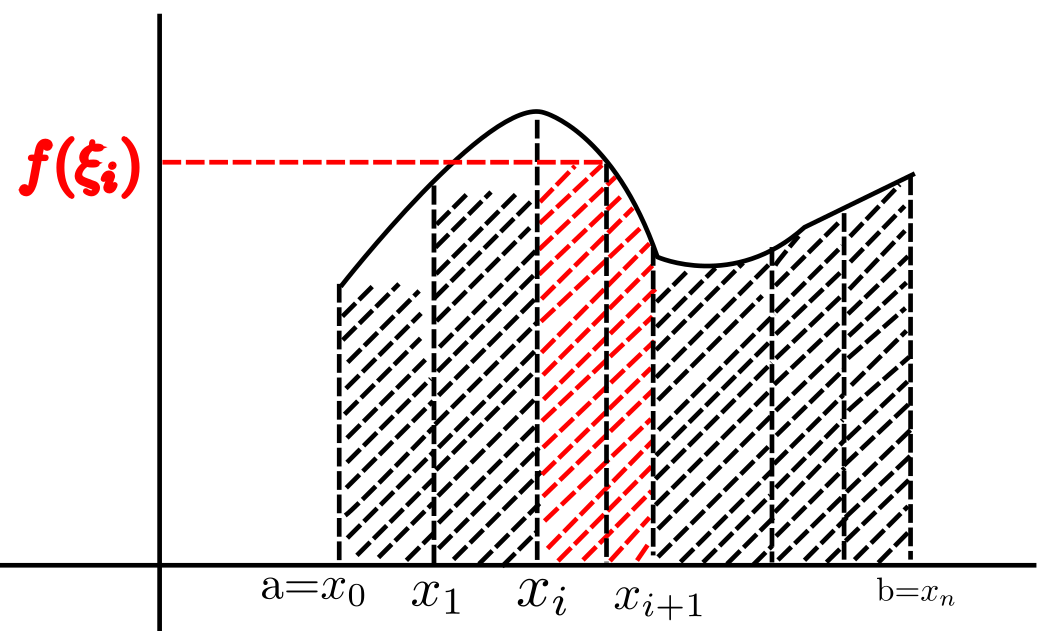
\includegraphics[max size={15cm}{10cm}]{6.1.1.png}
    \end{center}
    \indent Пусть $f(x)\geq 0$\\
    \begin{enumerate}
        \item Произведём разбиение $[a; b]$ - $R$.\\
        $a=x_0<x_1<\dots<x_n=b$
        \item В каждом элементарном отрезке $[x_i;x_{i+1}]$ произвольным образом выберем точку $\xi_i$.
        \item Вычислим $f(\xi_i)$.
        \item Вычислим $f(\xi_i) \Delta x_i$.
        \item Вычислим $\sigma_R = \sum_{i=0}^{n-1} f(\xi_i) \Delta x_i$.
        \item Обозначим $\lambda_R$ - диаметр разбиения.\\
        $\sigma_R=[x_i;x_i+1]$\\
        Пусть $\sigma_R \to 0$.\\
        Вычислим $\lim_{n \to \infty} \sigma_R = S$.
    \end{enumerate}
    
    \subsubsection*{Вычисление массы неоднородного тонкого стержня}
    \begin{center}
        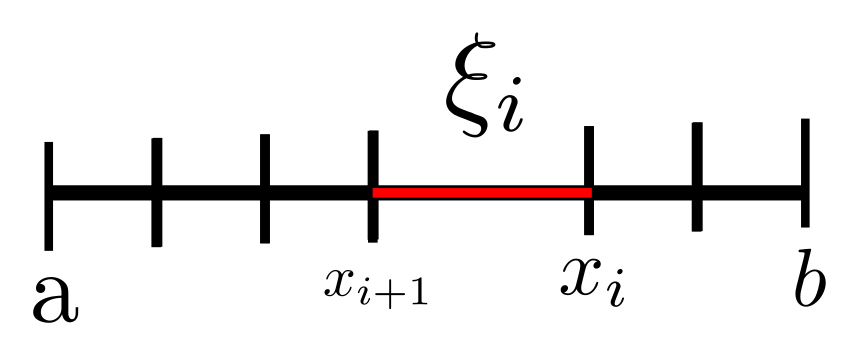
\includegraphics[max size={15cm}{10cm}]{6.2.1}
    \end{center}\noindent
    $\rho(\xi_i)$. Пусть $\rho = const = \rho (\xi_i)\;\;\forall x \in [x_i;x_{i+1}]$\\
    $m_i=\rho(\xi_i) \Delta x_i$\\
    \[m \approx \sum_{i} \rho(\xi_i) \Delta x_i=\sigma_R; m=\lim_{n \to \infty} \sigma_R\]

    \subsection{Определение определённого интеграла}\noindent
    Пусть на $[a;b]$ задана функция $f(x)$\\
    \begin{enumerate}
        \item Произведём разбиение отрезка $[a;b]$ - R.\\
        $R: a=x_0<x_1<\dots<x_n=b$. Пусть $\lambda_r = \underset{i}{max}[x_i;x_{i+1}]$ - диаметр разбиения.
        \item В каждом элементарном [$x_i;x_{i+1}$] произвольным образом выберем $\xi_i$.
        \item Вычислим $f(\xi_i)\Delta x_i$.
        \item Составим $\sigma_R=\sum_{i=0}^{n-1} f(\xi_i) \Delta x_i$ - интегральная сумма.
        \item Если $\exists$ \underline{конечный} предел интегральной суммы $\sigma_R$ при $\lambda_r \to 0$, не зависящий от способа разбиения $[a;b]$ и выбора точки $\xi_i$, то он называется \textbf{определённым интегралом} от функции $f(x)$ на $[a;b]$.
    \end{enumerate}\noindent
    \underline{Обозначение:} 
    \[\lim_{\sigma_R \to 0} \sigma_R = \int_{a}^{b} f(x)dx\]

    \subsubsection*{Определение определённого интеграла на языке "$\varepsilon - \delta$"}\noindent
    Число I называется \textbf{определённым интегралом} от функции $f(x)$
    на $[a;b]$, если 
    \[\forall \varepsilon>0 \,\exists\, \delta = \delta(\varepsilon)>0: 
    \forall \lambda_r < \delta \implies |I-\sigma_R | <\varepsilon\]

    \subsection{Необходимое условие интегрируемости функции}
    \subsubsection*{Теорема 6.3.1 (необходимое условие интегрируемости функции)}\label{th:6.3.1}
    Если функция интегрируема на некотором отрезке, то она ограничена на нём.\par\noindent
    \underline{Доказательство:}
    \begin{adjustwidth}{1.5em}{1.5em}
        Пусть $f(x)$ интегрируема на $[a;b]$ и $I = \int_{a}^{b} f(x)dx$ ($\exists$ конечное число).\\
        Зафиксируем $\varepsilon$. Тогда по определению $\exists$ $\delta: \lambda_r < \delta \implies |\sigma_R - I| < \varepsilon$.\\
        $I-\varepsilon < \sigma_R < I+\varepsilon$ - множество интегральных сумм.\\
        $\sigma_R$ ограничено.\\
        Пойдем от противного: пусть $f(x)$ интегрируема на $[a;b]$, но не ограничена на нём.\\
        Произведем разбиение отрезка $[a;b]$ - $R$.\\
        Т.к. $f(x)$ неограниченна на $[a;b] \implies f$ неограниченна по крайней мере на одном из элементарных отрезков $[x_i;x_{i+1}]$.\\
        Пусть для определённости этот отрезок $[x_0;x_1]$.\\
        Тогда $\forall n \in N \,\,\exists \,\xi^{(n)}_0: f(\xi^{(n)}_0)>n$, $\xi^{(n)}_0 \in [x_0;x_1]$.\\
        Тогда $\lim_{n \to \infty} f(\xi^{(n)}_0) = \infty$\\
        Составим $\sigma_R$:
        \[ \sigma_R = f(\xi^{(n)}_0) \Delta x_o + \sum_{i=1}^{n} f(\xi_i) \Delta x_i \]
        \[ \lim_{n \to \infty} \sigma_R = \infty \]
        Т.е. $\sigma_R$ неограниченна. Получили противоречие, следовательно, $f(x)$ ограничена.
        \begin{center}
            \textbf{Ч.т.д.}
        \end{center}
    \end{adjustwidth}\noindent
    \underline{Замечание:} Ограниченность функции является необходимым условием, но не является достаточным.\\
    Если функция ограничена, она не обязана быть интегрируемой. (!!!)\\
    \underline{Пример:} Функция Дирихле́\\
    \begin{adjustwidth}{1.5em}{1.5em}
        $f(x) = \begin{cases}
            1,x \in Q\\
            0,x \in I
        \end{cases}$
        \begin{enumerate}
            \item $[a;b]$ $R$\\
            Пусть точка $\xi_i \in Q \implies f(\xi_i) = 1 \implies \sum_{i=0}^{n} f(\xi_i) \Delta x_i =
            \sum_{i=0}^{n} \Delta x_i = b-a$\\
            \[\lim_{\lambda_R \to 0} \sigma_R = \lim_{\lambda_R \to 0} (b-a) = b-a\]
            \item $[a;b]$ $R$\\
            Пусть точка $\xi_i \in I \implies f(\xi_i)=0$\\
            \[\sigma_R = \sum_{i=0}^{n} f(\xi_i) \Delta x_i =0\]\\
            \[\lim_{\lambda_R \to 0} \sigma_R = 0\]\\
            \[\lim_{\lambda_R \to 0} \sigma_R = \nexists\]
        \end{enumerate}
    \end{adjustwidth}

    \subsection{Суммы Дарбу}
    \begin{center}
        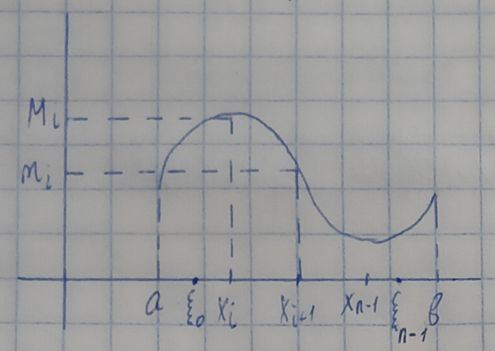
\includegraphics[max size={15cm}{10cm}]{6.4.1.png}
    \end{center}\noindent
    Пусть $f(x)$ задана на $[a;b]$ и ограничена на нём.\\
    $R: a=x_0<x_1<\dots<x_n=b$\\
    Пусть $m_i = \underset{x \in [x_i;x_{i+1}]}{\inf f(x)}$, $M_i = \underset{x \in [x_i;x_{i+1}]}{\sup f(x)}$.\\
    Составим $\sigma_R$:
    \[ \sigma_R = \sum_{i=0}^{n-1} f(\xi_i) \Delta x_i \]
    Рассмотрим:\\
    \begin{center}
        \textbf{Суммы Дарбу:} $\begin{cases}
            \underline{S_R} = \sum_{i=0}^{n-1} m_i \Delta x_i\\
            \overline{S_R} = \sum_{i=0}^{n-1} M_i \Delta x_i
        \end{cases}$
    \end{center}
    Очевидно, что $\underline{S_R} \leq \sigma_R \leq \overline{S_R}$\\
    Суммы Дарбу - необязательно интегрируемые суммы.\\
    \subsubsection*{Свойства сумм Дарбу:}
    \begin{enumerate}
        \item Нижняя (верхняя) сумма Дарбу является точный нижней (верхней) гранью интегральным сумм Римана, соответствующих данному разбиению R.\par\noindent
        \underline{Доказательство:}
        \begin{adjustwidth}{1.5em}{1.5em}
            \[ \underline{S_R} = \sum_{i = 0}^{n-1} m_i \Delta x_i = \sum_{i = 0}^{n - 1}\underset{\xi_i \in \Delta x_i}{\inf f(\xi_i)\Delta x_i} = \underset{\xi_i \in \Delta x_i}{\inf} \sum_{i = 0}^{n - 1} f(\xi_i)\Delta x_i = \underset{\xi_i \in \Delta x_i}{\inf} \sigma_R\]
        \end{adjustwidth}
        \item Если к имеющимся у разбиения $R$ точкам деления добавить новые точки, то верхняя сумма Дарбу не возрастает, а нижняя сумма Дарбу не убывает.\par\noindent
        \underline{Доказательство:}
        \begin{adjustwidth}{1.5em}{1.5em}
            \underline{Замечание:} для доказательства достаточно показать, что свойство выполняется при добавлении одной точки.\\
            Пусть $\overline{S_R}$ - верхняя сумма Дарбу, отвечающая разбиению $R$\\
            Пусть $\overline{S'_R}$ - верхняя сумма Дарбу, отвечающая разбиению $R'$, $R'=R+$добавленная точка.\\
            $\overline{S_R}$ будет отличаться от $\overline{S'_R}$ тем, что вместо слагаемого $M_i \Delta x_i$ будут $M_i'(x'-x_i)+M_i''(x_{i+1}-x')$
            \[\underset{x \in [x_i;x']}{M_i' = \sup f(x)}\]
            \[ \underset{x \in [x_i;x']}{M_i''= \sup f(x)}\]
            Т.к. $[x_i; x'] \subset [x_i; x_{i+1}]$, $[x'; x_{i+1}] \subset [x_i; x_{i+1}]$, то $M_i' \leq M_i$, $M_i''\leq M_i$\\
            Получим, что $M_i'(x'-x_i)+M_i''(x_{i+1}-x') \leq M_i(x'-x_i+x_{i+1}-x') = M_i(x_{i+1}-x_i)$\\
            Т. е. $\overline{S_R'} \leq \overline{S_R}$\\
            Аналогично $\underline{S_R'} \leq \underline{S_R}$
            \begin{center}
                \textbf{Ч.т.д.}
            \end{center}
        \end{adjustwidth}
        \item Каждая нижняя сумма Дарбу не больше любой верхней.\par\noindent
        \underline{Доказательство:}
        \begin{adjustwidth}{1.5em}{1.5em}
            Рассмотрим $R_1,R_2$ - различные разбиения\\
            Составим новое разбиение $R_3=R_1+R_2$\\
            \[\underline{S_{R_1}} \underset{\text{св-во 2}}{\leq} \underline{S_{R_3}} \underset{\text{по определению}}{\leq} \overline{S_{R_3}} \leq \overline{S_{R_2}}\]
            \begin{center}
                \textbf{Ч.т.д.}
            \end{center}
        \end{adjustwidth}\noindent
        \underline{Замечание:} Множество нижних сумм Дарбу $\{\underline{S_R}\}$ всегда ограничено какой-либо верхней суммой Дарбу. Значит это множество ограничено сверху. Тогда $\exists$ точная верхняя грань множества нижних сумм Дарбу:
        \[ \underset{R}{\sup} \underline{S_R} = I_* \]
        Аналогично $\exists\,I^* = \underset{R}{\inf} \overline{S_R}$\\
        $I_* \leq I^* \;\; \forall R$\\
        $\underline{S_R} \leq I_* \leq I^* \leq \overline{S_R}$
        \item \subsubsection*{Теорема 6.4.1 (о существовании интеграла)}\label{th:6.4.1}
        Для того, чтобы определённый интеграл, ограниченный функции $f(x)$ существовал $\Longleftrightarrow$\\
        $\lim_{\lambda_R \to 0} (\overline{S_r}- \underline{S_r})=0$, т.е. $\lim_{\lambda_R \to 0}\sum_{i=0}^{n-1} \omega_i \Delta x_i$ \par\noindent
        \underline{Доказательство:}
        \begin{adjustwidth}{1.5em}{1.5em}
            \textbf{Докажем необходимость ($\Rightarrow$)}\\
            Пусть определённый интеграл от ограниченной функции $f(x)$ $\exists$ на $[a;b]$\\
            Тогда
            \[ \lim_{\lambda_R \to 0} \sigma_R = I\]
            Т.е. 
            \[ \forall \varepsilon > 0\,\exists\,\delta > 0: \lambda_R < \delta \Rightarrow |\sigma_R - I| < \varepsilon \]
            \[ I - \varepsilon < \sigma_R < I+\varepsilon \;\;\; \forall R \]
            Т.е.
            \[ \left.\begin{matrix}
                I-\varepsilon < \underline{S_r}<I+\varepsilon \Rightarrow \lim_{\lambda_R \to 0} \underline{S_r}=I\\
                I-\varepsilon < \overline{S_R} < I + \varepsilon \Rightarrow \lim_{\lambda_R} \overline{S_r} = I\\
            \end{matrix}\right\rbrace \lim_{\lambda_R}(\overline{S_r}-\underline{S_r})=0\]\noindent
            \textbf{Докажем достаточность ($\Leftarrow$)}\\
            Пусть $\lim_{\lambda_R \to 0}(\overline{S_R}-\underline{S_R})=0$\\
            Т. е. $\lim_{\lambda_R \to 0} \overline{S_R} = \lim_{\lambda_R \to 0} \underline{S_R}$\\
            $\{\overline{S_R}\}$ невозрастающая, ограниченная снизу, т.е. $\lim_{\lambda_R} \overline{S_R} = I^*$\\
            Аналогично $\lim_{\lambda_R} \underline{S_R} = I_*$. Тогда $I^* = I_* = I$.\\
            \begin{center}
                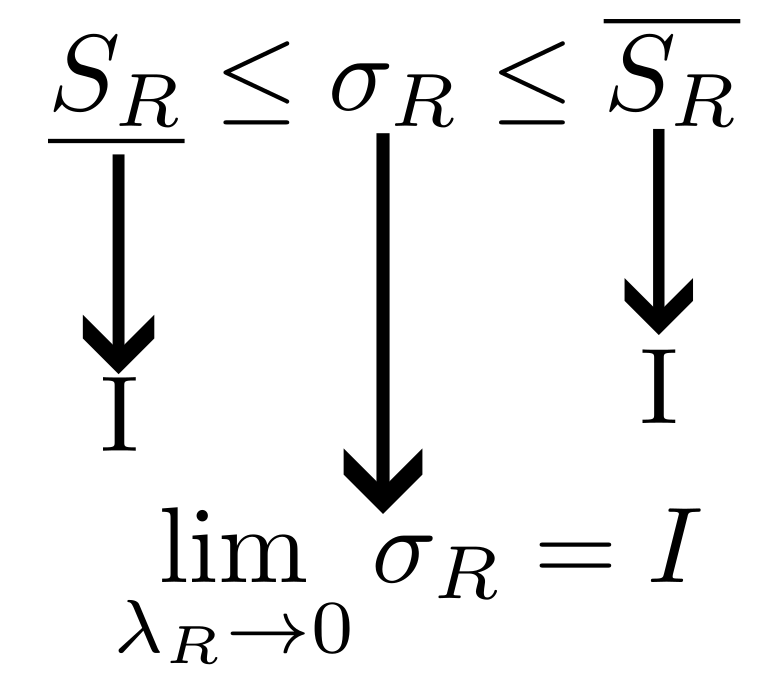
\includegraphics[scale=0.5]{6.4.2.png}
            \end{center}
            \begin{center}
                \textbf{Ч.т.д.}
            \end{center}
        \end{adjustwidth}
    \end{enumerate}
    \subsection{Достаточное условия интегрируемости функций}
    \subsubsection*{Теорема 6.5.1}\label{th:6.5.1}
    Функция, непрерывная на отрезке, интегрируема на нём.\par\noindent
    \underline{Доказательство:}
    \begin{adjustwidth}{1.5em}{1.5em}
        Если $f(x)$ непрерывна на $[a; b]$, то она равномерно непрерывна на нём.\\
        Тогда
        \[\forall\varepsilon>0\,\exists\,\delta>0:\forall x',x'' \in [a;b]: |x'-x''|<\delta \Rightarrow |f(x')-f(x'')|<\varepsilon\]
        Произведём разбиение $R: \lambda_R < \delta$\\
        Тогда 
        \[\forall x',x'' \in [x_i;x_{i+1}] \;\; |x'-x''| \leq x_{i+1}-x_i=\Delta x_i < \delta \Rightarrow |f(x')-f(x'')|<\varepsilon \]
        Рассмотрим колебание функции $f(x)$ на элементарном отрезке: $\omega_i=M_i-m_i = \underset{\Delta x_i}{\sup}f(x)-\underset{\Delta x_i}{\inf}f(x) \fbox{=}$\\
        \underline{Замечание:}
        \begin{gather*}
            \underset{[a;b]}{\sup} \lambda f(x) = \lambda \underset{[a;b]}{\inf} f(x),\lambda < 0\\
            \underset{[a;b]}{\sup}(f(x)-g(x))=\underset{[a;b]}{\sup} (f(x)+\underset{[a;b]}{\sup} (-g(x))) = \underset{[a;b]}{\sup} f(x)-\underset{[a;b]}{\inf} g(x)\\
        \end{gather*}
        $\fbox{=} \underset{x',x'' \in \Delta x}{\sup}|f(x')=f(x'')|<\varepsilon$\\
        \begin{center}
            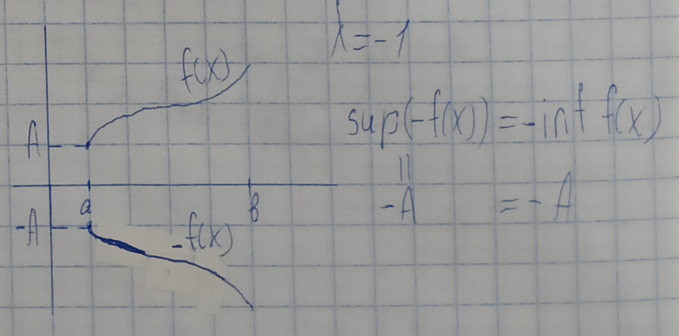
\includegraphics[max size={15cm}{10cm}]{6.5.1.png}\\
        \end{center}
        Рассмотрим 
        \[ \sum_{i=0}^{n-1} \omega_i \Delta x_i < \varepsilon \sum_{i=0}^{n-1} \Delta x_i = \varepsilon (b-a) \]
        $\lim_{\lambda_R \to 0} \sum_{i=0}^{n-1} \omega_i \Delta x_i = 0 \implies f(x)$ интегрируема на $[a; b]$\\
        \begin{center}
            \textbf{Ч.т.д.}
        \end{center}
    \end{adjustwidth}

    \subsubsection*{Теорема 6.5.2}\label{th:6.5.2}
    Ограниченная монотонная функция на отрезке интегрируема на нём.\par\noindent
    \underline{Доказательство:}
    \begin{adjustwidth}{1.5em}{1.5em}
        Пусть для определённости $f(x)$ возрастает на $[a;b]$
        \[ f(a)<f(x)<f(b) \;\; \forall x \in (a;b)\]
        \begin{gather*}
            m_i=\underset{[x_i;x_{i+1}]}{\inf}f(x) = f(x_i)\\
            M_i = \underset{[x_i;x_{i+1}]}{\sup}f(x)=f(x_{i+1})\\
            \overline{S_R}-\underline{S_R}=\sum_{i=0}^{n-1} (M_i-m_i) \Delta x_i = \sum_{i=0}^{n-1}(f(x_{i+1})-f(x_i))\Delta x_i < \sum_{i=0}^{n-1}(f(x_{i+1}-f(x_i)))\delta =\\
            = (\cancel{f(x_1)} - f(x_0) + \cancel{f(x_2)} - \cancel{f(x_1)} + \cancel{f(x_3)} - \cancel{f(x_2)} + \dots + f(x_n) - \cancel{f(x_n - 1)})\delta =\\
            = (f(x_n)-f(x_o))\delta = (f(b)-f(a))\delta \fbox{=}
        \end{gather*}
        Пусть $\delta=\frac{\varepsilon}{f(b)-f(a)} \fbox{=} \varepsilon$.\\
        Т.е. $\lim_{\lambda_R \to 0}(\overline{S_R}-\underline{S_R})=0$.\\
        Т.е. $f(x)$ интегрируема на $[a; b]$.
        \begin{center}
            \textbf{Ч.т.д.}
        \end{center}
    \end{adjustwidth}
    \underline{Замечание:}
    Монотонные функции могут быть разрывными.\\
    Т.е. по \hyperref[th:6.5.2]{теореме 6.5.2} $\exists$ разрывные интегрируемые функции.
    \begin{center}
        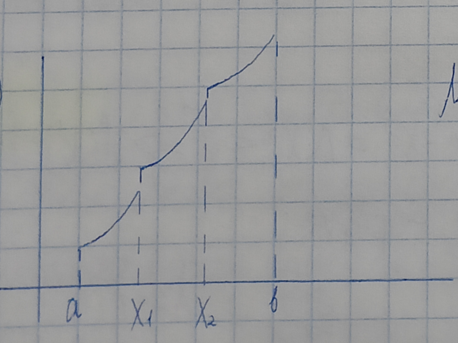
\includegraphics[max size={15cm}{10cm}]{6.5.2.png}
    \end{center}

    \subsection{Свойства интегрируемых функций}
    \begin{enumerate}
        \item \[ \int_{a}^{b} dx = b-a \]
        \[ \int_{a}^{b} dx = \int_{a}^{b} 1*dx \]
        \[ \sigma_R = \sum_{i=0}^{n-1} f(\xi_i)\Delta x_i=\sum_{i=0}^{n-1}\Delta x_i=b-a \]
        $\lim_{\lambda_R \to 0} \sigma_R=b-a$
        \item Если $f(x)$ интегрируема на каждом из $[a; c]$, $[c; b]$ $(a<c<b)$, то она интегрируема на $[a;b]$
        \[ \int_{a}^{b}f(x)dx=\int_{a}^{c}f(x)dx+\int_{c}^{b}f(x)dx \]
        \underline{Доказательство:}\\
        \begin{adjustwidth}{1.5em}{1.5em}
            а)
            \begin{center}
                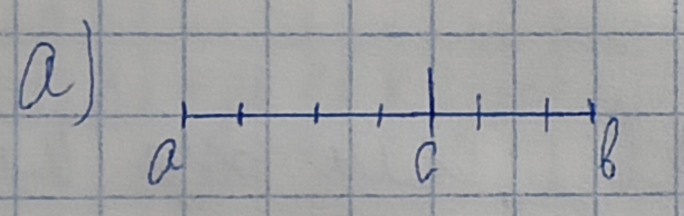
\includegraphics[max size={15cm}{10cm}]{6.6.1.png}\\
            \end{center}
            Произведем разбиение $R$ $[a;b]$\\
            $R$: $a=x_0<x_1<\dots<x_m=c<\dots<x_n=b$\\
            Пусть $R_1: a=x_0<x_1<\dots<x_m=c$\\
            $R_2:c=x_m<x_{m+1}<\dots<x_n=b$\\
            Составим $\sigma_R$\\
            \begin{gather*}
                \sigma_R = \sum_{i=0}^{n-1}f(\xi_i)\Delta x_i=\sum_{i=0}^{m-1}f(\xi_i)\Delta x_i+\sum_{i=m}^{n-1}f(\xi_i)\Delta x_i=\sigma_{R_1}+\sigma_{R_2}\\
                \lim_{\lambda_R \to 0}\sigma_R=\lim_{\lambda_R \to 0}(\sigma_{R_1}+\sigma_{R_2})=
                \begin{vmatrix}
                    \text{Если } \lambda_R \to 0 \Rightarrow \\
                    \lambda_{R_1} \to 0, \lambda_{R_2} \to 0
                \end{vmatrix} =\\
                = \lim_{\lambda_R \to 0}\sigma_{R_1}=\lim_{\lambda_R \to 0}\sigma_{R_2} =
                \int_{a}^{c}f(x)dx+\int_{c}^{b}f(x)dx\\
            \end{gather*}
            \begin{center}
                a)
                \textbf{Ч.т.д.}
            \end{center}
            б) Пусть $R$ - произвольное разбиение, не содержащее точку $C$.\\
            $R'$ - разбиение, содержащее точку $C$.\\
            Пусть известно $\lim_{\lambda_R \to 0}\sigma_{R'}=I$. Покажем, что $\lim_{\lambda_R \to 0}\sigma_R=I \; \forall R$\par\noindent
            Пусть 
            \[ R: a=x_0<x_1<\dots<\underset{x_m < c < x_{m+1}}{x_m<x_{m+1}}< \dots <x_n=b \]
            \begin{center}
                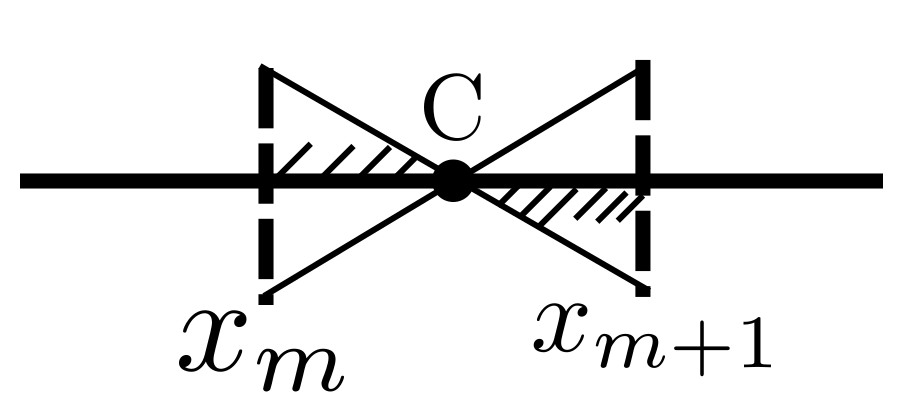
\includegraphics[max size={15cm}{10cm}]{6.6.2.png}
            \end{center}
            \[ \sigma_{R'}=\sigma_R-f(\xi_m)(x_{m+1}-x_m)+f(\xi_m')(c-x_m)+f(\xi_m'')(x_{m+1}-c) \implies \sigma_R=\sigma_{R'}+A\]
            Рассмотрим
            \begin{gather*}
                |A|=|f(\xi_m)(x_{m+1}-x_m)+f(\xi_m')(c-x_m)+f(\xi_m'')(x_{m+1}-c)| \leq\\
                \leq |M(x_{m+1}-x_m)+M(c-x_m)+M(x_{m+1}-C)|=|2M(x_{m+1}-x_m)|\\ 
                \lim_{\lambda_R \to 0}|A|=0 \;\;\; \lim_{\lambda_R \to 0} \sigma_R = \lim_{\lambda_R \to 0}(\sigma_{R'}+A) = \lim_{\lambda_R \to 0}\sigma_{R'}+\lim_{\lambda_R \to 0}A =
                \begin{vmatrix}
                    \text{Если } \lambda_R \to 0, \\
                    \text{то} \lambda_R' \to 0
                \end{vmatrix} =\\
                = \lim_{\lambda_R \to 0}\sigma_{R'} +\lim_{\lambda_R \to 0}A=I
            \end{gather*}
            \begin{center}
                б)
                \textbf{Ч.т.д.}
            \end{center}
        \end{adjustwidth}
        \textbf{Следствие:} Из 2 следует интегрируемость кусочно-непрерывных функций.\\
        Функция называется кусочно-непрерывной на $[a; b]$ если она имеет на нём \underline{конечное} число точек разрыва I рода.\\
        На концах отрезка функция может быть не определена.\\
        Т.е. $f(x)$ кусочно-непрерывна, если $\exists$ $R$ такое, что $\forall$ точек $x_k \;\;\; k=\overline{0,n-1}$ $\exists$ конечные пределы $\lim_{x \to x_k+0} f(x)$, $\lim_{x\to x_k-0}f(x)$
        В точке $x_k$ $f(x)$ может быть определена, или нет.\\
        \begin{center}
            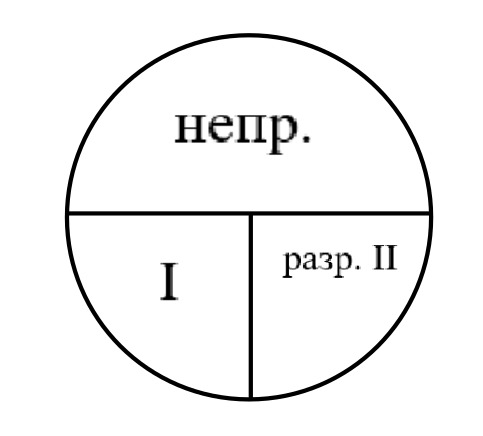
\includegraphics[max size={15cm}{10cm}]{6.6.3.png}\\
            \begin{math}
                f_k(x)=\begin{cases}
                    f(x_k+0),x=x_k\\
                    f(x),x_k<x<x_{k+1}\\
                    f(x_{k+1}-0),x=x_{k+1}\\
                \end{cases}
            \end{math}
        \end{center}
        Тогда для таких функций свойство 2 выполняется.\\
        $f_k$ в точке $x_k$ может быть неопределенна.\\
        В этой случае нужно доопределить $f(x)$ в этих точках, т.е. 
        \[ \int_{a}^{b} f(x) dx=\sum_{k=0}^{n-1}\int_{x_k}^{x_{k+1}}f_k(x)dx\]
        \item Если функции $f(x)$ и $g(x)$ интегрируемы на $[a; b]$, то $\forall \lambda , \mu$ функция $\lambda f+\mu g$ также интегрируема на $[a; b]$.
        \[ \int_{a}^{b}[\lambda f(x) + \mu g(x)]dx=\lambda \int_{a}^{b}f(x)dx + \mu \int_{a}^{b} g(x) dx \]
        \underline{Доказательство:}
        \begin{adjustwidth}{1.5em}{1.5em}
            Пусть $R$ - произвольное разбиение\\
            \begin{gather*}
                \sigma_R(\lambda f(x) + \mu g(x))=\sum_{i=0}^{n-1}(\lambda f(\xi_i) + \mu g(\xi_i))\Delta x_i =\\
                = \lambda \sum_{i=0}^{n-1} f(\xi_i) \Delta x_i +
                \mu \sum_{i=0}^{n-1} g(\xi_i)\Delta x_i =\\
                = \lambda \sigma_R(f)+\mu\sigma_R(g)    
            \end{gather*}
            
            Т.к. $f(x)$ и $g(x)$ интегрируемы на $[a; b]$, то $\exists$ конечный предел правой части $\implies$ $\exists$ конечный предел и левой части: 
            \[ \lim_{\lambda_R \to 0}\sigma_R (\lambda f + \mu g) = \lambda \lim_{\lambda_R \to 0}\sigma_R(f)+\mu \lim_{\lambda_R \to 0}\sigma_R(g) \]
            \[ \int_{a}^{b}[\lambda f(x)+\mu g(x)]dx=\lambda \int_{a}^{b}f(x)dx+\mu \int_{a}^{b} g(x)dx \]
            \begin{center}
                \textbf{Ч.т.д.}
            \end{center}
        \end{adjustwidth}
        \item Интегрируемость произведения интегрируемых функций: Если $f(x)$ и $g(x)$ интегрируемы на $[a; b]$, то их произведение тоже интегрируемо.\\
        \underline{Доказательство:}
        \begin{adjustwidth}{1.5em}{1.5em}
            Если $f(x)$ и $g(x)$ интегрируемы на $[a; b]$, то они ограничены на нём (по необходимому условию интегрируемости).\\
            Т.е. 
            \[ \forall x \in [a;b] \;\;\; |f(x)|\leq A,|g(x)|\leq A \implies |f(x)g(x)|\leq A^2\]
            Т.е. $|f(x)g(x)|$ ограничены.\\
            \underline{Замечание:}\\
            Рассмотрим 
            \begin{gather*}
                f(x')g(x')-f(x)g(x)=f(x')g(x')-f(x)g(x)-f(x)g(x')+f(x)g(x') =\\
                = (f(x')-f(x))g(x')+(g(x')-g(x))f(x)\\
                |f(x')g(x')-f(x)g(x)| \leq |f(x')-f(x)||g(x')|+|g(x')-g(x)||f(x)| \leq\\
                \leq A(|f(x')-f(x)|+|g(x')-g(x)|)\\
            \end{gather*}
            Введем разбиение $R$ и выберем точку $x$ и $x'$ в одном и том же отрезке разбиения $[x_k;x_{k+1}]$ 
            \[ \omega_k(fg)\leq A(\omega_k(f)+\omega_k(g)) \]
            Т.е. 
            \[\sum_{k=0}^{n-1} \omega_k (fg) \Delta x_k \leq A \sum_{k=0}^{n-1}\omega_k(f)\Delta x_k+A\sum_{i=0}^{n-1}\omega_k(g)\Delta x_k\]
            Переходя к lim при $\lambda_k \to 0$, получим $\lim_{\lambda_R \to 0} \sum_{k=0}^{n-1} \omega_k(fg) \Delta x_k=0$, т.е. $f(x)g(x)$ интегрируема на $[a; b]$ по \hyperref[th:6.4.1]{теореме 6.4.1}.
            \begin{center}
                \textbf{Ч.т.д.}
            \end{center}
        \end{adjustwidth}
        \item $\int_{a}^{a} f(x)dx=0 \;\;\; (\Delta x_i=0)$
        \item $\int_{a}^{b} f(x)dx=-\int_{b}^{a} f(x)dx \;\;\; (x_{k+1}-x_k=-(x_k-x_{k+1}))$
    \end{enumerate}
    
    \subsection{Оценки интегралов. Формулы среднего значения.}
    \begin{enumerate}
        \item Оценки интегралов:\\
        \begin{adjustwidth}{1.5em}{1.5em}
            a) Если $f(x)$ интегрируема и $\forall x \in [a;b] f(x)\geq 0,\text{ то } \int_{a}^{b} f(x)dx \geq 0$\\
            \underline{Доказательство:}
            \begin{adjustwidth}{1.5em}{1.5em}
                Составим 
                \[ \sigma_R=\sum_{k=0}^{n-1} f(\xi_k)\Delta x_k \geq 0 \]
                \[ \lim_{\lambda_R \to 0}\sigma_R=\int_{a}^{b}f(x)dx\geq 0 \]
                \begin{center}
                    \textbf{Ч.т.д.}
                \end{center}
            \end{adjustwidth}
            \textbf{Следствие:} Если $f(x)$ и $g(x)$ интегрируемы на $[a;b]$ и $\forall x \in [a;b]\; f(x)\geq g(x)$, то $\int_{a}^{b}f(x)dx \geq \int_{a}^{b} g(x)dx$\\
            \underline{Доказательство:}
            \begin{adjustwidth}{1.5em}{1.5em}
                Рассмотрим 
                \[ f(x)-g(x)\geq 0 \overset{a)}{\implies} \int_{a}^{b} (f(x)-g(x))dx \geq 0 \]
                \[ \int_{a}^{b} f(x)dx-\int_{a}^{b}g(x)dx\geq 0 \text{ (св-во 3) } \implies \int_{a}^{b}f(x)dx\geq\int_{a}^{b}g(x)dx\]
                \begin{center}
                    \textbf{Ч.т.д.}
                \end{center}
            \end{adjustwidth}
            б) Если $f(x)$ интегрируема на $[a;b]$, то $\left|f(x)\right|$ тоже интегрируема на $[a;b]$ и $\left|\int_{a}^{b}f(x)dx\right|\leq \int_{a}^{b}\left|f(x)\right| dx$\\
            \underline{Доказательство:}
            \begin{adjustwidth}{1.5em}{1.5em}
                \begin{gather*}
                    \sigma_R=\sum_{k=0}^{n-1} f(\xi_k)\Delta x_k\\
                    |\sigma_R|=\left|\sum_{k=0}^{n-1} f(\xi_k)\Delta x_k\right| \leq \sum_{k=0}^{n-1}|f(\xi_k)|\Delta x_k
                    =\sigma_R(|f|)\\
                    \lim_{\lambda_R \to 0}|\sigma_R|=\left|\int_{a}^{b}f(x)dx\right|\leq \lim_{\lambda_R \to 0}\sigma_R (|f|)=\int_{a}^{b}|f(x)|dx\\
                \end{gather*}
            \end{adjustwidth}
        \end{adjustwidth}
        \item Непрерывность интегралов:\\
        Функция $F(x) = \int_{a}^{x}f(t)dt$ - функция с \textbf{переменным верхним пределом}.
        \begin{center}
            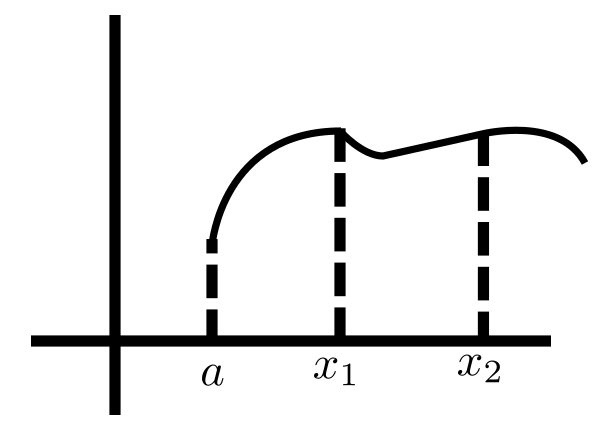
\includegraphics[max size={15cm}{10cm}]{6.7.1.png}
        \end{center}
        Аналогично $G(x) = \int_{x}^{b}f(t)dt$ - функция с \textbf{переменным нижним пределом}.
    \end{enumerate}
    \subsubsection*{Теорема 6.7.1}\label{th:6.7.1}
    Если функция $f(x)$ интегрируема на $[a;b]$, то $F(x), G(x)$ непрерывны на $[a;b]$.\par\noindent
    \underline{Доказательство:}
    \begin{adjustwidth}{1.5em}{1.5em}
        Д-во проведем для $F(x)$.\par\noindent
        $f(x)$ ограничена на $[a;b]$ (необходимое условие интегрируемости), т.е. $\forall x \in [a;b]$ $|f(x)|\leq C$
        \[ F(x+\Delta x)=\int_{a}^{x+\Delta x}f(t)dt= \int_{a}^{x} f(t)dt+\int_{x}^{x+\Delta x}f(t)dt \]
        Рассмотрим 
        \begin{gather*}
            \Delta F(x) = F(x + \Delta x) - F(x)=\int_{a}^{x} f(t)dt+\int_{x}^{x+\Delta x}f(t)dt-\int_{a}^{x}f(t)dt=
            \int_{x}^{x+\Delta x}f(t)dt\\
            \left|\Delta F(x)\right| = \left| \int_{x}^{x+\Delta x }f(x)dt\right| \leq \mathbb{C} \left|\int_{x}^{x+\Delta x}dt\right|= \mathbb{C} \left|\Delta x\right|
        \end{gather*}
        $\lim_{\Delta x \to 0}|\Delta F(x)| = 0 \Rightarrow \lim_{\Delta x \to 0}\Delta F(x)=0 \Rightarrow F(x)$ непрерывна в точке $x$.\\
        Т.к. $x$ - производная точек $[a; b] \Rightarrow F(x)$ непрерывна на $[a;b]$.
        \begin{center}
            \textbf{Ч.т.д.}
        \end{center}
        \textbf{Следствие:} Если $f(x)$ интегрируема на $[a;b]$ (и непрерывна на нём), то $\lim_{\varepsilon \to 0} \int_{a+\varepsilon}^{b-\varepsilon}f(x)dx=\int_{a}^{b}f(x)dx$.\\
        \underline{Доказательство:}
        \begin{adjustwidth}{1.5em}{1.5em}
            \begin{gather*}
                \lim_{\varepsilon \to 0} \int_{a+\varepsilon}^{b-\varepsilon}f(x)dx = \lim_{\varepsilon \to 0}\left(\int_{a+\varepsilon}^{c}f(x)dx+\int_{c}^{b-\varepsilon}f(x)dx\right) =\\
                = \lim_{\varepsilon \to 0} \int_{a+\varepsilon}^{c} f(x)dx+\lim_{\varepsilon \to 0}\int_{c}^{b-\varepsilon}f(x)dx = \int_{a}^{c} f(x)dx+\int_{c}^{b} f(x)dx = \int_{a}^{b}f(x)dx
            \end{gather*}
            \begin{center}
                \textbf{Ч.т.д.}
            \end{center}
        \end{adjustwidth}
    \end{adjustwidth}
    \subsubsection*{Теорема 6.7.2 (интегральная теорема о среднем)}\label{th:6.7.2}
    Пусть $f(x)$ и $g(x)$ интегрируемы на $[a;b]$, $\forall x \in [a;b]\;\; m \leq f(x) \leq M$ $g(x)$ не меняет знак на $[a;b]$\\
    Тогда $\exists \mu : m\leq \mu \leq M: \int_{a}^{b} f(x)g(x)dx = \mu \int_{a}^{b}g(x)dx$.\par\noindent
    \underline{Доказательство:}
    \begin{adjustwidth}{1.5em}{1.5em}
        \begin{gather*}
            m \leq f(x) \leq M\;\;\;\; \Big| \times g(x)\\
            g(x)\geq 0 : mg(x)\leq f(x)g(x)\leq Mg(x) \implies\\
            \implies m \int_{a}^{b} g(x) dx \leq \int_{a}^{b}f(x)g(x)dx \leq M \int_{a}^{b}g(x)dx \;\;\;\; \Big| : \int_{a}^{b} g(x)dx\\
            g(x)\leq 0 : mg(x)\geq f(x)g(x)\geq Mg(x) \implies\\
            \implies m \int_{a}^{b} g(x) dx \geq \int_{a}^{b}f(x)g(x)dx \geq M \int_{a}^{b}g(x)dx \;\;\;\; \Big| : \int_{a}^{b} g(x)dx\\
        \end{gather*}
        Если $\int_{a}^{b} g(x)dx = 0 \implies \int_{a}^{b} f(x)g(x)dx =0$ в обоих случаях и $\mu$ любое. 
        \begin{center}
            \textbf{Ч.т.д.}
        \end{center}
        Если $\int_{a}^{b} g(x) dx \ne 0$ при 
        \[ \begin{matrix}
            g(x) > 0 \implies \int_{a}^{b} g(x)dx >0\\
            g(x)<0 \implies \int_{a}^{b} g(x)dx<0
        \end{matrix} \]
        Разделим на $\int_{a}^{b} g(x)dx$, в обоих случаях получим: 
        \[ m \leq \frac{\int_{a}^{b}f(x)g(x)dx}{\underbrace{\int_{a}^{b}g(x)dx}_{\mu}}\leq M \]
        \[ m\leq \mu \leq M \] 
        \[ \int_{a}^{b} f(x)g(x)dx=\mu\int_{a}^{b}g(x)dx \]
        \begin{center}
            \textbf{Ч.т.д.}
        \end{center}
        \textbf{Следствие:} При дополнительно условии о том, что $f(x)$ непрерывна на $[a;b]$, тогда на $(a;b)$ $\exists$ точка $\xi$ такая, что $\int_{a}^{b}f(x)g(x)dx=f(\xi)\int_{a}^{b}g(x)dx$.\\
        В частности, пусть $g(x)=1$.
        \[ \int_{a}^{b} f(x) dx=f(\xi)(b-a) \implies f(\xi)= \boxed{\frac{1}{b-a}\int_{a}^{b}f(x)dx} \text{ - формула среднего значения} \]
        \[ f(\xi)=\frac{\int_{a}^{b} f(x)dx}{b-a} \]
        \begin{center}
            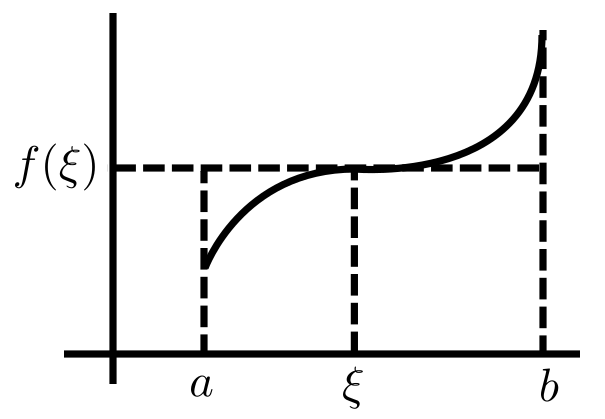
\includegraphics[max size={15cm}{10cm}]{6.7.2.png}
        \end{center}
        \underline{Доказательство:}
        \begin{adjustwidth}{1.5em}{1.5em}
            Если $\int_{a}^{b} g(x)dx=0$, то верно $\forall \xi$\\
            Пусть $\int_{a}^{b} g(x)dx \not = 0$ и для определенности $g(x)>0$.
            \[ m \le f(x) \le M \]
            \[ \underset{x \in [a; b]}{m = \inf f(x)} \;\;\;\; \underset{x \in [a; b]}{M = \sup f(x)} \]
            И по \hyperref[th:6.7.2]{интегральной теореме о среднем (6.7.2)} $m \leq \mu \leq M$.
            \begin{adjustwidth}{1.5em}{1.5em}
                1-й случай:\\
                Пусть $m<\mu<M$\\
                По 2-ой теореме Вейерштрасса (3.8.2) $\exists\,\alpha, \beta \in [a;b]: f(\alpha) = m,f(\beta) = M$\\
                Тогда по теореме Больцано-Коши (3.8.3) $\exists$ точка $\xi$ такая, что:
                \[ m < f(\xi) < M \]
                \[ m < \mu < M \;\;\;\; \mu = f(\xi) \]
                \begin{center}
                    1) \textbf{Ч.т.д.}
                \end{center}
                2-й случай:\\
                $\mu=M \text{ или } \mu=m$\\
                Пусть для определенности $\mu=M$\\
                Покажем, что и в этом случае на $(a;b)$ $\exists$ точка $\xi$ такая, что $f(\xi)=\mu=M$.\\
                Предположим противное: пусть на $(a;b)$ $\nexists$ точка $\xi$ такая, что $f(\xi)=\mu=M$.\\
                Тогда своего наибольшего значения $f(x)$ достигает в какой-либо точке или $x=a$, или $x=b$.\\
                Рассмотрим $[a+\varepsilon; b-\varepsilon]$: $f(x)$ непрерывна на нём $\implies$ по 2-ой теореме Вейерштрасса (3.8.2) $\exists$ точка $x_0$, в которой $f(x)$ достигает своего наибольшего значения.\\
                Тогда 
                \[ M-f(x_0)=\underset{x \in [a+\varepsilon; b-\varepsilon]}{\min(M - f(x))} \]
                Т.к. $\mu=M$, то по \hyperref[th:6.7.2]{интегральной теореме о среднем (6.7.2)}: 
                \[ \int_{a}^{b} f(x)g(x)dx=M\int_{a}^{b}g(x)dx \implies \overbrace{\int_{a}^{b}(M-f(x))g(x)dx=0} \]
                Рассмотрим 
                \[ \int_{a}^{b}(M-f(x))g(x)dx\geq\int_{a+\varepsilon}^{b-\varepsilon}(M-f(x))g(x)dx \geq (M-f(x_0)) \underbrace{\int_{a+\varepsilon}^{b-\varepsilon} g(x)dx>0}_{>0} \]
                Получили противоречие $\implies \exists$ точка $\xi \in (a;b)$ такая, что $f(\xi)=M=\mu$.
                \begin{center}
                    2) \textbf{Ч.т.д.}
                \end{center}
            \end{adjustwidth}
        \end{adjustwidth}
    \end{adjustwidth}
    \subsubsection*{Теорема 6.7.3 (дифференцирование интеграла по верхнему пределу)}\label{th:6.7.3}
    Если $f(x)$ интегрируема на $[a;b]$ и непрерывна в точке $x_0 \in [a;b]$, то $F(x)=\int_{a}^{x}f(t)dt$ дифференцируема в этой точке и $F'(x_0)=f(x_0)$. \par\noindent
    \underline{Доказательство:}\\
    \begin{adjustwidth}{1.5em}{1.5em}
        \begin{gather*}
            \lim_{\Delta x \to 0}  \frac{\Delta F}{\Delta x} = F'(x_0)\\
            \Delta F=\int_{x_0}^{x_0+\Delta x}f(t)dt \;\;\;\; x_0 \in [a;b],x_0+\Delta x \in [a;b]\\
            \frac{1}{\Delta x}\int_{x_0}^{x_0+\Delta x}dt=1
        \end{gather*}
        \underline{Замечание:} рассмотрим 
        \begin{gather*}
            \left|\frac{\Delta F}{\Delta X}-f(x_0)\right| = \left|\frac{1}{\Delta x}\int_{x_0}^{x_0+\Delta x}f(t)dt-\frac{f(x_0)}{\Delta x}\int_{x_0}^{x_0+\Delta x}dt\right| =\\
            = \left|\frac{1}{\Delta x}\int_{x_0}^{x_0+\Delta x}(f(t)-f(x_0))dt\right| \leq \frac{1}{|\Delta x|}\left|\int_{x_0}^{x_0+\Delta X}\left|f(t)-f(x_0)\right|dt\right| \fbox{<}\\
        \end{gather*}
        Т.к. $f(x)$ непрерывна в точке $x_0$, то $\forall \varepsilon > 0\,\exists\,\delta>0:|x-x_0|<\delta \implies |f(x)-f(x_0)|<\varepsilon$\\
        Пусть $|\Delta x| < \delta$. Тогда $\forall t \in [x_0;x_0+\Delta x]$:
        \[ |t-x_0| \leq |\Delta x| < \delta \implies \left|f(t)-f(x_0)\right| < \varepsilon \]
        \[ \fbox{<} \frac{\varepsilon}{\Delta x}\left|\int_{x_0}^{x_0+\Delta x}dt\right|=\varepsilon.\]
        Т.е. 
        \[ \lim_{\Delta x \to 0} \frac{\Delta F}{\Delta x} = F'(x_0)=f(x_0) \]
        \begin{center}
            \textbf{Ч.т.д.}
        \end{center}
    \end{adjustwidth}
    \underline{Замечание:} рассмотрим
    \begin{align*}
        &\int_{a}^{b} f(x)dx=\int_{a}^{b}f(t)dt & &\\
        &\int_{a}^{b} f(t)dt=\int_{a}^{x}f(t)dt+\int_{x}^{b} f(t)dt & &x \in (a;b)\\
        &\int_{a}^{b} f(t) dt = F(x)+G(x) & &G'(x)=-F'(x)\\
        &0=F'(x)+G'(x) & &G'(x_0)=-F'(x_0)=-f(x_0)
    \end{align*}

    \subsection{Существование первообразных для непрерывных функций. Основные правила интегрирования.}
    \subsubsection*{Теорема 6.8.1 (о существовании первообразной для непрерывной функции)}\label{th:6.8.1}
    Если $f(x)$ непрерывна $\forall x \in [a;b]$, то на $[a; b]$ у нее $\exists$ первообразная.\\
    Если $x_0$ - произвольная: $x_0 \in [a;b]$, то $F(x)=\int_{x_0}^{x}f(t)dt$ является одной из первообразных на $[a;b]$\par\noindent
    \underline{Доказательство:}
    \begin{adjustwidth}{1.5em}{1.5em}
        Для доказательства надо показать, что $F'(x)=f(x)$. Смотреть доказательство \hyperref[th:6.7.3]{теоремы дифференцирования интеграла по верхнему пределу (6.7.3)}\\
        ($F'(x_0)=f(x_0)$, но т.к. $x_0$ - произвольная: $x_0 \in [a;b]$, то это равенство выполняется $\forall x \in [a;b]$).
        \begin{center}
            \textbf{Ч.т.д.}
        \end{center}
    \end{adjustwidth}
    \underline{Замечание:} $F(x)=\int_{x_0}^{x}f(t)dt$\\
    Если $x>x_0, \;\;\; F'(x)=f(x)$\\
    Если $x<x_0, \;\;\; F'(x)=\left[-\underbrace{\int_{x}^{x_0}f(t)dt}_{G(x)}\right]'=-(-f(x))=f(x)$\par\noindent
    \underline{Замечание:} $\int f(x)dx=F(x)+\mathbb{C}$\\
    \[ \underset{\text{связь между неопределенным и определённым интегралом}}{\int f(x)dx = \int_{x_0}^{x}f(t)dt+\mathbb{C}} \]
    \subsubsection*{Теорема 6.8.2 (основная теорема интегрального исчисления)}\label{th:6.8.2}
    Если $f(x)$ непрерывна на $[a; b]$, то какова бы не была на $[a;b]$ её первообразная $\Phi(x)$, то справедлива формула 
    \[ \int_{a}^{b}f(x)dx=\Phi(x)\Big|^{b}_{a}=\Phi(b)-\Phi(a) \text{ - \underline{формула Ньютона-Лейбница}} \]\par\noindent
    \underline{Доказательство:}\\
    \begin{adjustwidth}{1.5em}{1.5em}
        По \hyperref[th:6.8.1]{теореме о существовании первообразной для непр. функции (6.8.1)} $F(x)=\int_{a}^{x} f(t)dt$ является первообразной для $f(x)$ на $[a;b]$\\
        Т.к. $F(x)$ и $\Phi(x)$ - две первообразные для одной и той же $f(x)$ на $[a;b]$, то
        \begin{gather*}
            F(x)=\Phi(x)+\mathbb{C}\\
            \int_{a}^{x}f(t)dt = \Phi(x) + \mathbb{C}\\
        \end{gather*}
        Пусть $x=a \;\;\;\;\; 0=\Phi(а)+\mathbb{С} \implies \mathbb{C}=-\Phi(а)$. Тогда $\int_{a}^{x}f(t)dt=\Phi(x)-\Phi(а)$.\\
        Пусть $x=b \;\;\;\;\; \int_{a}^{b} f(t)dt=\Phi(b)-\Phi(а)$.\\
        Если переобозначить, то 
        \[ \int_{a}^{b}f(x)dx=F(b)-F(a) \]
        \begin{center}
            \textbf{Ч.т.д.}
        \end{center}
    \end{adjustwidth}
    \subsubsection*{Теорема 6.8.3 (о замене переменной в определённом интеграле)}\label{th:6.8.3}
    Пусть $f(x)$ задана на $\Delta x$, $x=\varphi(t)$ задана на $\Delta t$.\\
    $\varphi(\Delta t) \subset \Delta x$, т.е. задана сложная функция $f(\varphi(t))$.\\ Если $f(x)$ непрерывна на $\Delta x$, а $\varphi(t)$ и $\varphi'(t)$ непрерывны на $\Delta t$, то 
    \[ \int_{a}^{b}f(x)dx=\int_{\alpha}^{\beta}f(\varphi(t))\varphi'(t)dt \;\;\;\;\; a=\varphi(\alpha), b=\varphi(\beta) \]\noindent
    \underline{Доказательство:}
    \begin{adjustwidth}{1.5em}{1.5em}
        Пусть $F(x)$ - является первообразной для $f(x)$ на $[a;b]$.
        \[ \int_{a}^{b} f(x)dx=F(x)\Big|^{b}_{a} \]
        \[ (F(\varphi(t)))'=F'(\varphi(t))\varphi'(t)=f(\varphi (t))\varphi'(t) \]
        Т.е. $F(\varphi(t))$ является первообразной для $f(\varphi(t))\varphi'(t) $ на $[\alpha; \beta]$.
        \[ \int_{\alpha}^{\beta}f(\varphi(t))\varphi'(t)dt=F(\varphi(t))\Big|^{\beta}_{\alpha}=F(\varphi(\beta))-F(\varphi(\alpha))=F(b)-F(a)=\int_{a}^{b}f(x)dx \]
        \begin{center}
            \textbf{Ч.т.д.}
        \end{center}
    \end{adjustwidth}
    \subsubsection*{Теорема 6.8.4 (формула интегрирования по частям)}\label{th:6.8.4}
    Если $u(x)$, $u'(x)$, $v(x)$, $v'(x)$ непрерывны на $[a;b]$, то 
    \[ \int_{a}^{b} udv = uv \Big|^b_a-\int_{a}^{b}vdu \]\noindent
    \underline{Доказательство:}
    \begin{adjustwidth}{1.5em}{1.5em}
        \begin{gather*}
            (uv)'=u'v+uv'\\
            \int_{a}^{b} (uv)'dx=\int_{a}^{b} u'v dx+\int_{a}^{b}uv'dx\\
            uv \Big|^b_a=\int_{a}^{b}vdu + \int_{a}^{b} udv\\
            \int_{a}^{b}udv=uv\Big|^b_a-\int_{a}^{b} vdu
        \end{gather*}
        \begin{center}
            \textbf{Ч.т.д.}
        \end{center}
    \end{adjustwidth}

    \subsection{Геометрические приложения определённого интеграла. Площадь криволинейной трапеции.}
    \begin{enumerate}
        \item $f(x)$ задана явно на $[a; b]$\\
        Пусть $f(x) \geq 0$
        \begin{center}
            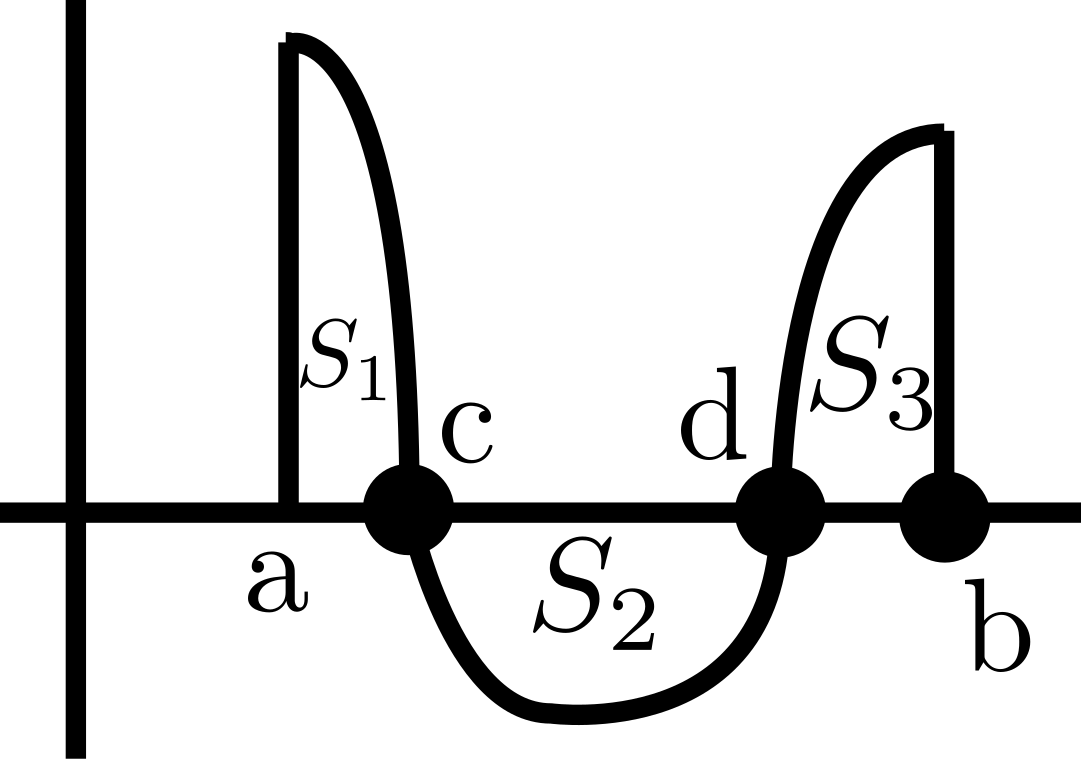
\includegraphics[max size={15cm}{10cm}]{6.9.1.png} 
        \end{center}
        $R: a=x_0<x_1<\dots<x_n=b$\\
        В каждом $[x_i; x_{i+1}]$ произвольно выберем точку $\xi_i$.\\
        Вычислим $f(\xi_i)$.\\
        Вычислим $f(\xi_i)\Delta x_i$.\\
        Составим $\sigma_R$:
        \[ \sigma_R = \sum_{i=0}^{n-1}f(\xi_i)\Delta x_i \]
        \[ \lim_{\lambda_R \to 0}\sigma_R=\int_{a}^{b} f(x)dx=S \]
        \[ S=S_1+S_2+S_3 \]
        \begin{center}
            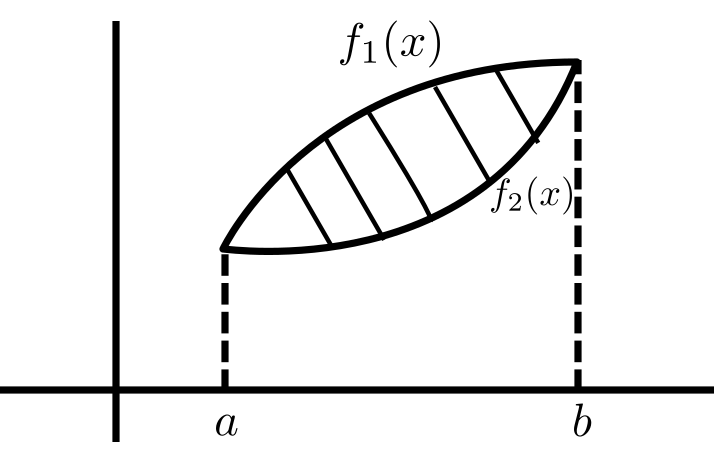
\includegraphics[max size={15cm}{10cm}]{6.9.2.png} 
        \end{center}
        \[S=\int_{a}^{b}(\underset{\text{большая}}{f_1(x)} - \underset{\text{меньшая}}{f_2(x)})dx\]
        \begin{center}
            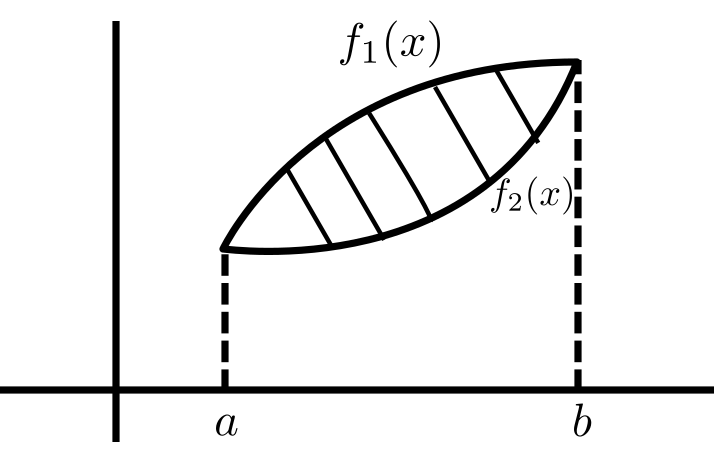
\includegraphics[max size={15cm}{10cm}]{6.9.3.png}
        \end{center}
        \item Если функция задана параметрически\\
        \begin{align*}
            \begin{cases}
                x=x(t)\\
                y=y(t)
            \end{cases} \;\;&\;\;\; \alpha \leq t \leq \beta
             & 
            \begin{cases}
                x=cos(t)\\
                y=sin(t)
            \end{cases} \;\;&\;\;\; 0 \leq t \leq 2 \pi
        \end{align*}
        \[ S=\int_{a}^{b} f(x)dx = \int_{a}^{b} ydx=
        \begin{vmatrix}
            x=x(t)\\
            a=x(\alpha)\\
            b=x(\beta)
        \end{vmatrix} = \boxed{\int_{\alpha}^{\beta}y(t)x'(t)dt=S} \]
        \item Вычисление площади криволинейной трапеции в полярной системе координат. \\
        Полярная система координат:
        \begin{gather*}
            \varphi \in [0; 2\pi]\\
            r \in [0; +\infty)\\
            \boxed{x = r\cos \varphi}\\
            \boxed{y = r\sin \varphi}
        \end{gather*}
        \begin{center}
            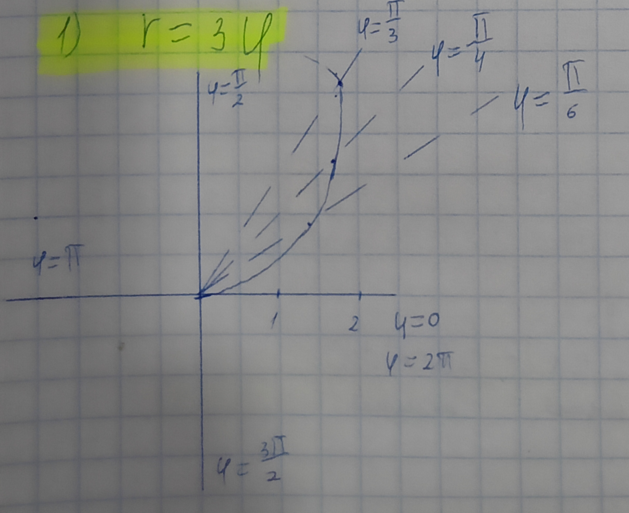
\includegraphics[max size={15cm}{10cm}]{6.9.4.png}
        \end{center}
        \[ y = kx \]
        \begin{center}
            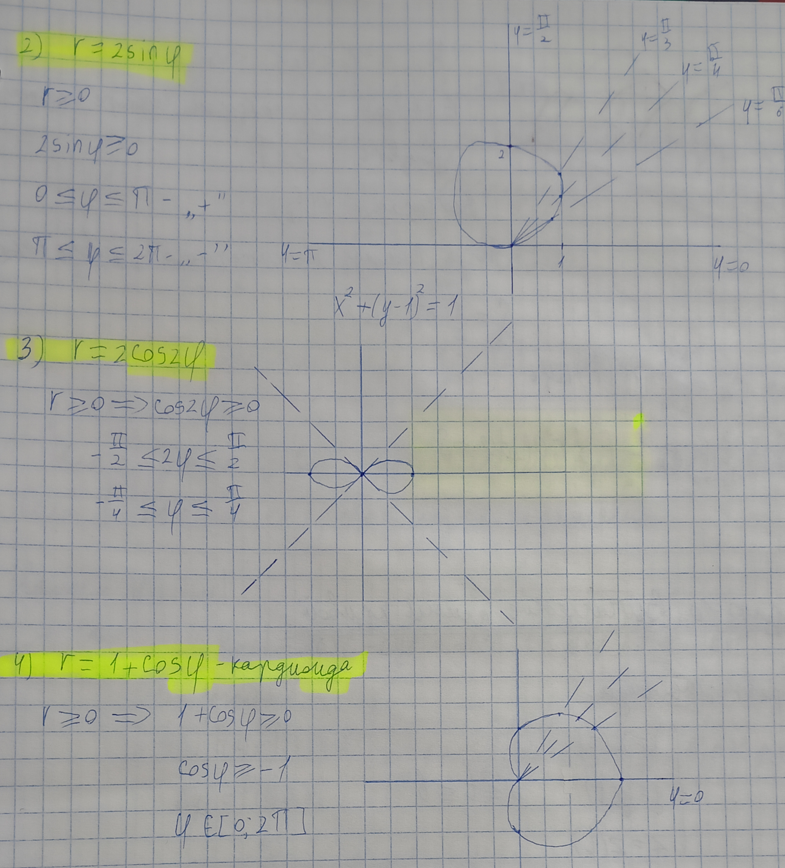
\includegraphics[max size={15cm}{10cm}]{6.9.5.png}
        \end{center}
        \[ r = a\varphi \;\;\; \varphi \in [0; 2\pi] \]
        \begin{center}
            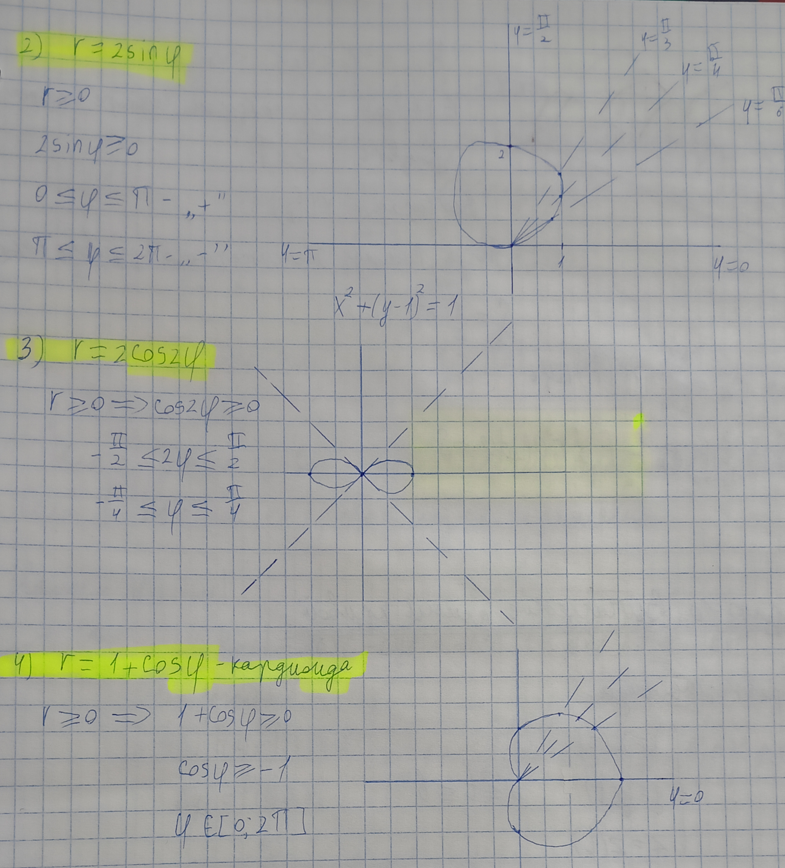
\includegraphics[max size={15cm}{10cm}]{6.9.6.png}
        \end{center}
        \begin{gather*}
            r = \sqrt{x^2 + y^2}\\
            \tg \varphi = \frac{y}{x}\\
            \varphi = \arctg \frac{y}{x}, \;\;\; (x, y) \in \text{ I, IV четв.}\\
            \varphi = \arctg \frac{y}{x} + \pi, \;\;\; (x, y) \in \text{ II, III четв.}\\
        \end{gather*}
        Некоторые кривые в полярной системе координат:
        \begin{enumerate}
            \item $r = 3\varphi$
            \begin{center}
                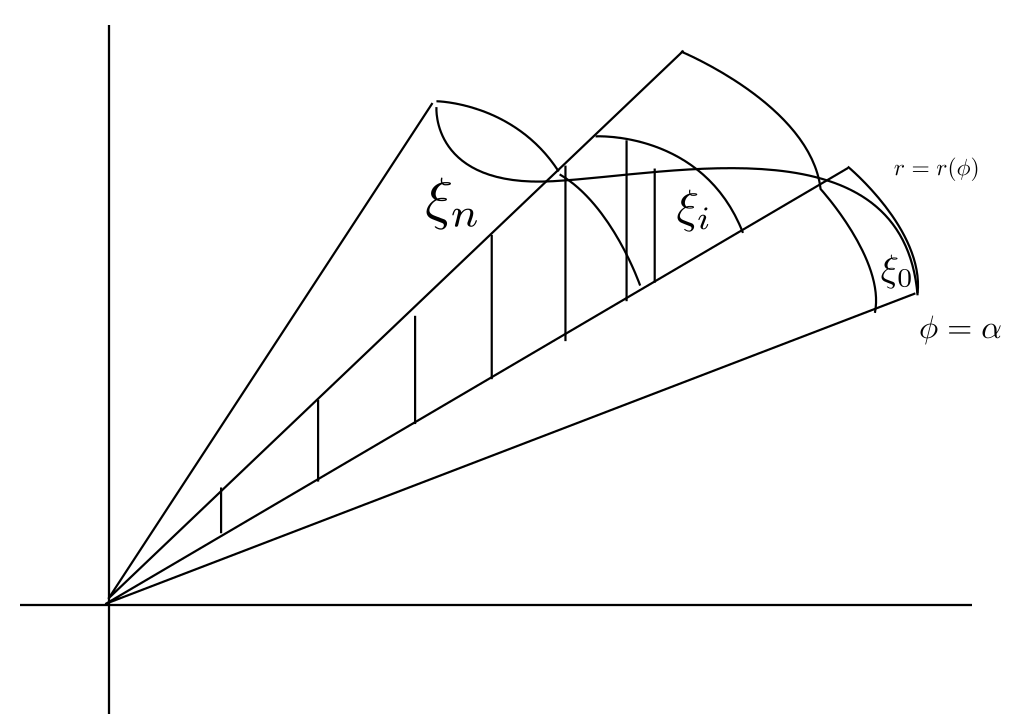
\includegraphics[max size={15cm}{10cm}]{6.9.7.png}\\
            \end{center}
            \item $r = 2 \sin \varphi$
            \begin{gather*}
                r \geq 0\\
                2 \sin \varphi \geq 0\\
                0 \leq \varphi \leq \pi \text{ - "+"}\\
                \pi \leq \varphi \leq 2\pi \text{ - "-"}
            \end{gather*}
            \begin{center}
                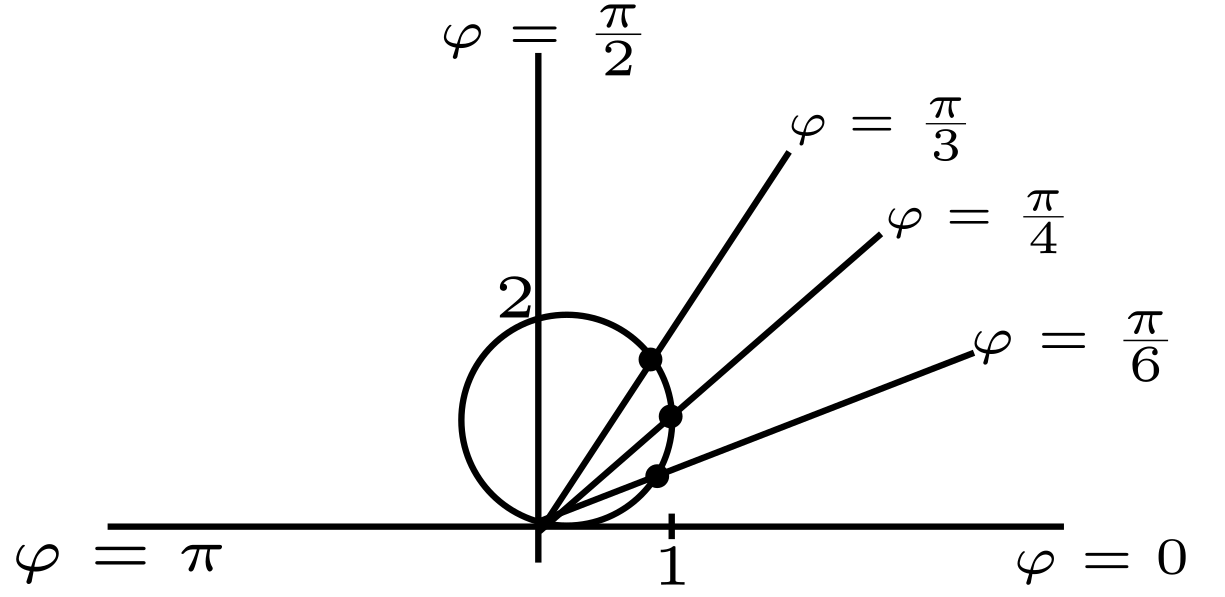
\includegraphics[max size={15cm}{10cm}]{6.9.8.png}
            \end{center}
            \item $r = 2 \cos 2\varphi$
            \begin{gather*}
                r \geq 0 \implies \cos 2 \varphi \geq 0\\
                -\frac{\pi}{2} \leq 2 \varphi \leq \frac{\pi}{2}\\
                -\frac{\pi}{4} \leq \varphi \leq \frac{\pi}{4}
            \end{gather*}
            \begin{center}
                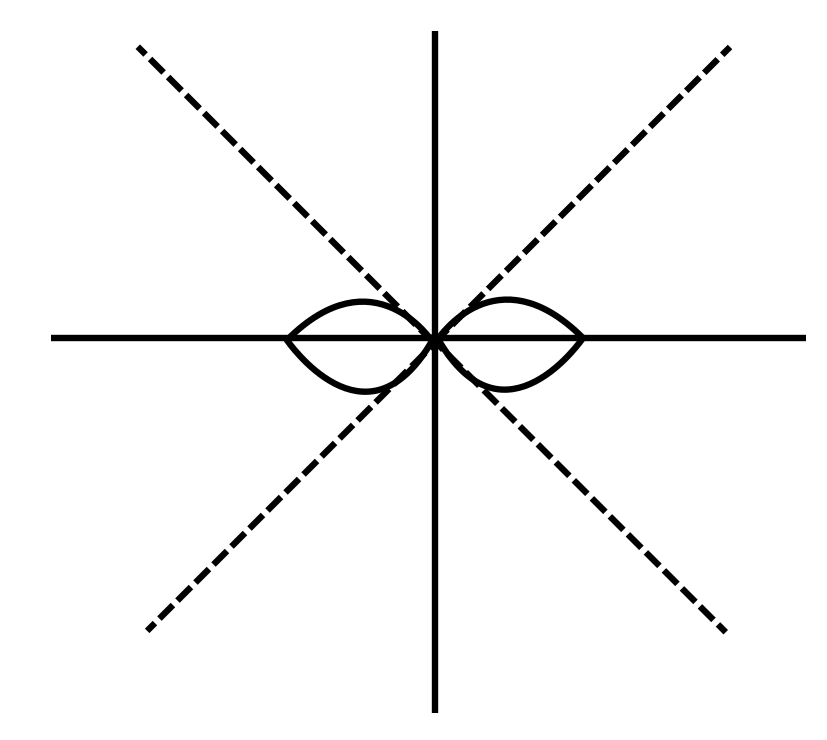
\includegraphics[max size={15cm}{10cm}]{6.9.9.png}
            \end{center}
            \item $r = 1 + \cos \varphi$ - кардиоида
            \begin{gather*}
                r \geq 0 \implies 1 + \cos \varphi \geq 0\\
                \cos \varphi \geq -1\\
                \varphi \in [0; 2\pi]
            \end{gather*}
            \begin{center}
                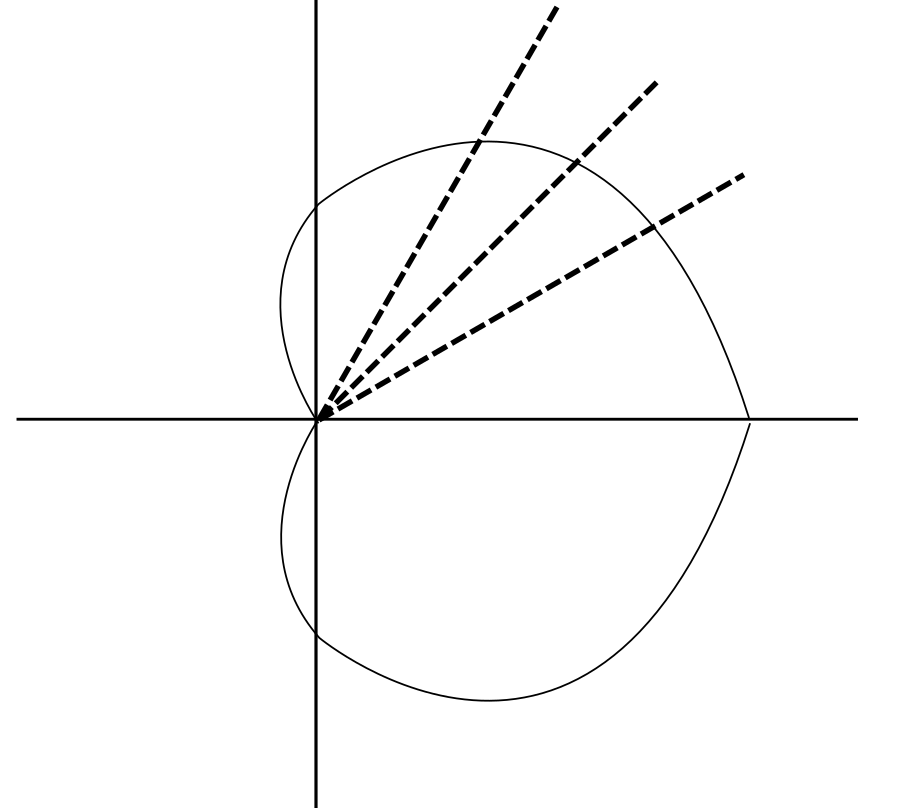
\includegraphics[max size={15cm}{10cm}]{6.9.10.png}
            \end{center}
        \end{enumerate}
        Как записать прямую в полярной системе координат?
        \begin{center}
            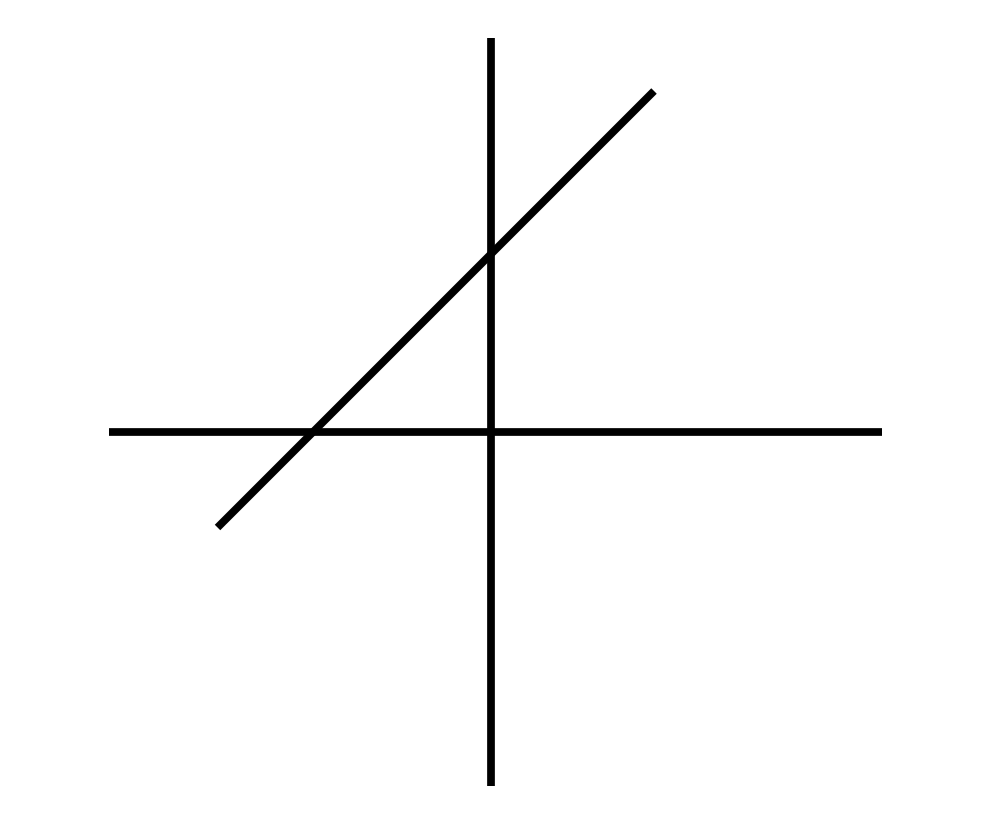
\includegraphics[max size={15cm}{10cm}]{6.9.11.png}
        \end{center}
        \begin{adjustwidth}{1.5em}{1.5em}
            \[ y = x + 1 \]
            \[ r \sin \varphi = r \cos \varphi + 1 \]
            \[ r (\sin \varphi - \cos \varphi) = 1 \]
            \[ r = \frac{1}{\sin \varphi - \cos \varphi} \]
        \end{adjustwidth}
        \underline{Площадь криволинейной трапеции в полярной системе координат:}\\
        Найти площадь криволинейной сектора, ограниченного дугой $r=r(\varphi)$ и двумя полярными радиусами $\varphi = \alpha$ и $\varphi = \beta$
        \begin{center}
            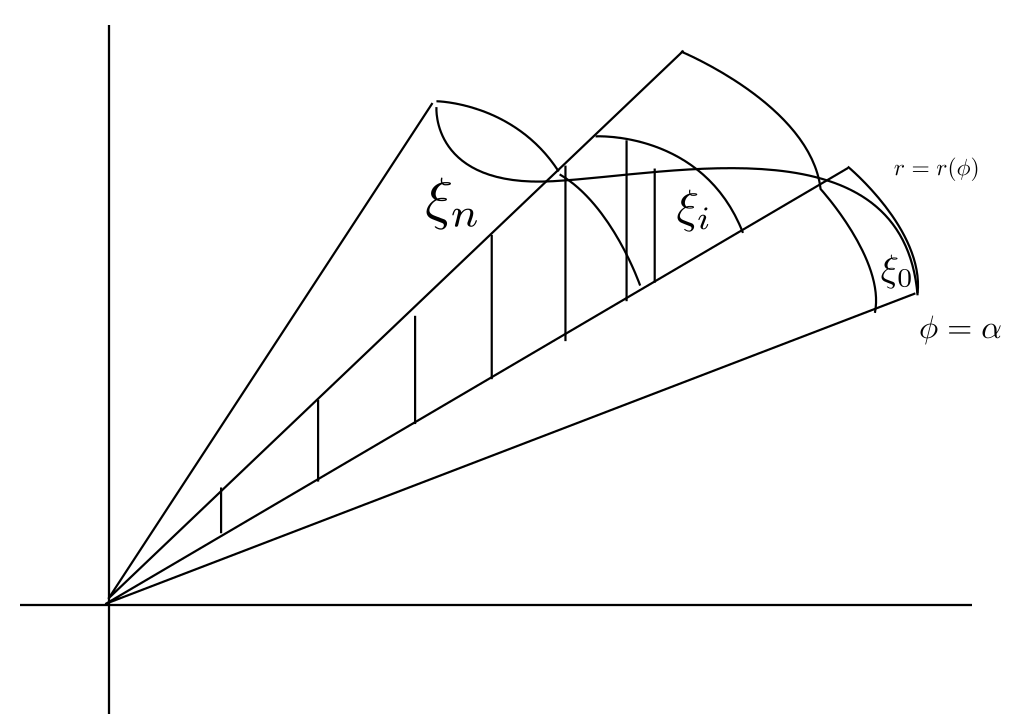
\includegraphics[max size={15cm}{10cm}]{6.9.12.png}
        \end{center}
        $R: \alpha=\varphi_0<\varphi_1<\dots<\varphi_n=\beta$\\
        В каждом элементарном секторе выберем произвольно $\varphi=\xi_i$.\\
        Вычислим $r(\xi_i)$.\\
        Тогда площадь элементарного кругового сектора: 
        \[ S_i=\frac{1}{2} r^2(\xi_i) \Delta \varphi_i \]
        Составим $\sigma_R$:
        \[ \sigma_R = \sum_{i=0}^{n-1} \frac{1}{2} r^2(\xi_i) \Delta \varphi_i \]
        Тогда 
        \[ S=\lim_{\lambda_R \to 0}\sigma_R = \boxed{ \int_{a}^{b}\frac{1}{2} r^2(\xi_i) \Delta \varphi_i=S }\]
    \end{enumerate}

    \subsection{Вычисление длины кривой.}\noindent
    Уравнения вида: 
    \[ \begin{cases}
        x=x(t)\\
        y=y(t)\\
        z=z(t)
    \end{cases} \;\;\;\;\; a\leq t \leq b \]
    \indent где $x(t)$, $y(t)$, $z(t)$ непрерывны определяют в пространстве \textbf{непрерывную кривую} $\Gamma$.\\
    Если функции $x(t)$, $y(t)$, $z(t)$ не только непрерывны, но и имеют непрерывные $x'(t)$, $y'(t)$, $z'(t)$, одновременно не образующиеся в ноль $\forall t \in [a;b] \;\;\; (x'(t)^2 + y'(t)^2 + z'(t)^2 \ne 0),$ то кривая называется \textbf{гладкой}.
    \begin{center}
        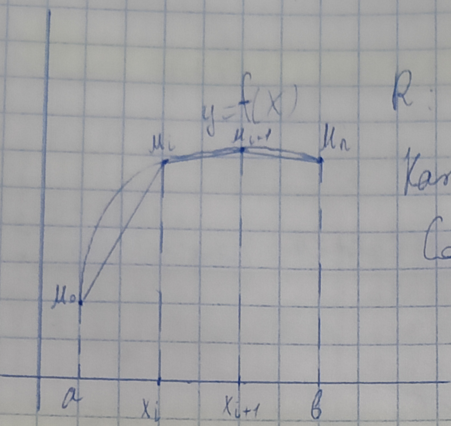
\includegraphics[max size={15cm}{10cm}]{6.10.1.png}
    \end{center}
    $ R: a=x_0<x_1<\dots<x_n=b $\\
    Каждой точке $x_i$ на кривой соответствует точке $M_i$. Соединим все соседние точки ломаными $M_iM_{i+1}$.
    \[ \left|\Gamma_n\right|=\sum_{i=0}^{n-1}\left|M_iM_{i+1}\right| \]
    Если $\exists$ конечный предел $\lim_{\lambda_R \to 0} \left|\Gamma_n\right|$, то он называется \textbf{длиной} кривой $y=f(x)$ на $[a; b]$\\
    Или: \textbf{длина} кривой - точная верхняя грань $\left|\Gamma_n\right| \;\;\; l=\sup\left|\Gamma_n\right|$\\
    Если $l$ - конечное, то кривая называется \textbf{спрямляемой}.\\
    Найдем $\left|M_iM_{i+1}\right|$:\\
    \begin{center}
        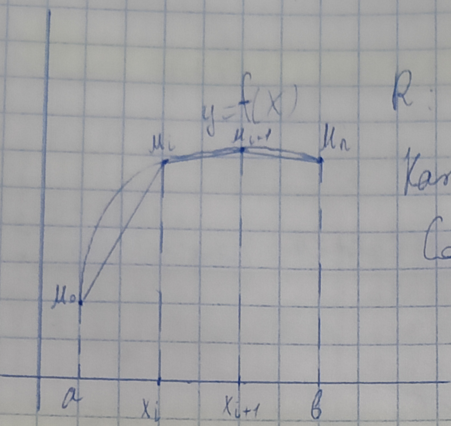
\includegraphics[max size={15cm}{10cm}]{6.10.1.png}
    \end{center}
    \begin{gather*}
        |M_iM_{i+1}|=\sqrt{\Delta x_i^2+\Delta y_i^2}=\sqrt{\Delta x_i^2\left(1+\frac{\Delta y_i^2}{\Delta x_i^2}\right)}+\sqrt{1+\frac{\Delta y_i^2}{\Delta x_i^2}} \times \Delta x_i =\\
        = \begin{vmatrix}
            \text{Теорема Лагранжа (4.12.4)}\\
            f(b)-f(a)=f'(\xi)(b-a)\\
            \Delta y_i=f'(\xi)\Delta x_i
        \end{vmatrix}=\sqrt{1+\frac{f'(\xi)^2 \Delta x_i^2}{\Delta x_i^2}}\Delta x_i=\sqrt{1+f'(\xi_i)^2}\Delta x_i
    \end{gather*}
    Составим $\sigma_R$:
    \[ \sigma_R = \sum_{i=0}^{n-1}\sqrt{1+f'(\xi_i)^2}\Delta x_i \]
    \underline{Замечание:} точка $\xi_i$ берётся из теоремы Лагранжа (4.12.4), но можно показать, что $\lim$ будет существовать при произвольном выборе точки $\xi_i$.\\
    Тогда 
    \[ \lim_{\lambda_R \to 0} \sigma_R = \boxed{ l =\int_{a}^{b} \sqrt{1+y'(x)^2}dx } \]
    \subsubsection*{Длина дуги для функции, заданной параметрически:}\noindent
    Пусть
    \[ \begin{cases}
        x=x(t)\\
        y=y(t)
    \end{cases} \;\;\;\;\; \alpha \leq t \leq \beta \]
    Пусть
    \[ x(\alpha)=a, x(\beta)=b \]
    Рассмотрим
    \begin{gather*}
        l=\int_{a}^{b} \sqrt{1+f'(x)^2}dx=
        \begin{vmatrix}
            x=x(t)\\
            dx=x'(t)dt\\
            x=a \implies t=\alpha\\
            x=b \implies t= \beta
        \end{vmatrix}=\int_{\alpha}^{\beta} \sqrt{1+(\frac{y'_t}{x'_t})^2}x'(t)dt =\\
        = \int_{\alpha}^{\beta} \sqrt{\frac{x'(t)^2+y'(t)^2}{x'(t)^2}}x'(t)dt = \boxed{ \int_{\alpha}^{\beta}\sqrt{x'(t)^2+y'(t)^2}dt = l }
    \end{gather*}
    \subsubsection*{Длина дуги для функции, заданной в полярной системе координат:}\noindent
    Пусть задана функция в виде
    \begin{align*}
        &r=r(\varphi) & &\alpha \leq \varphi \leq \beta & &r(\varphi)=r
    \end{align*}
    \begin{align*}
        &\begin{cases}
            x=rcos(\varphi)\\
            y=rsin(\varphi)
        \end{cases} & 
        &\begin{cases}
            x=r(\varphi)cos(\varphi)\\
            y=r(\varphi)sin(\varphi)
        \end{cases} & 
        &\begin{cases}
            x'=r'cos(\varphi)-rsin(\varphi)\\
            y'=r'sin(\varphi)+rcos(\varphi)
        \end{cases}
    \end{align*}
    \begin{gather*}
        x'^2=r'^2cos^2\varphi-2rr'sin(\varphi) cos(\varphi)+r^2sin^2\varphi\\
        y^2=r'^2sin^2\varphi+2rr'sin(\varphi) cos(\varphi) + r^2cos^2\varphi\\
        x'^2+y'^2=r'^2r^2
    \end{gather*}
    \[ \boxed{ l=\int_{\alpha}^{\beta} \sqrt{r^2(\varphi)+r'(\varphi)^2}d\varphi } \]
    \[ l=\int_{a}^{b}\sqrt{1+f'(x)^2}dx=\underset{(l)}{\int}dl \]
    \[ \underset{\text{дифференциал дуги}}{dl} = \sqrt{1+f'(x)^2}dx \]
    \[ dl=\sqrt{x'^2+y'^2}dt \]
    \[ dl=\sqrt{r^2+r'^2}d\varphi \]

    \subsection{Вычисление объема тела вращения}\noindent
    Пусть задана кривая $y=f(x) \;\;\; a\leq x\leq b$
    \begin{center}
        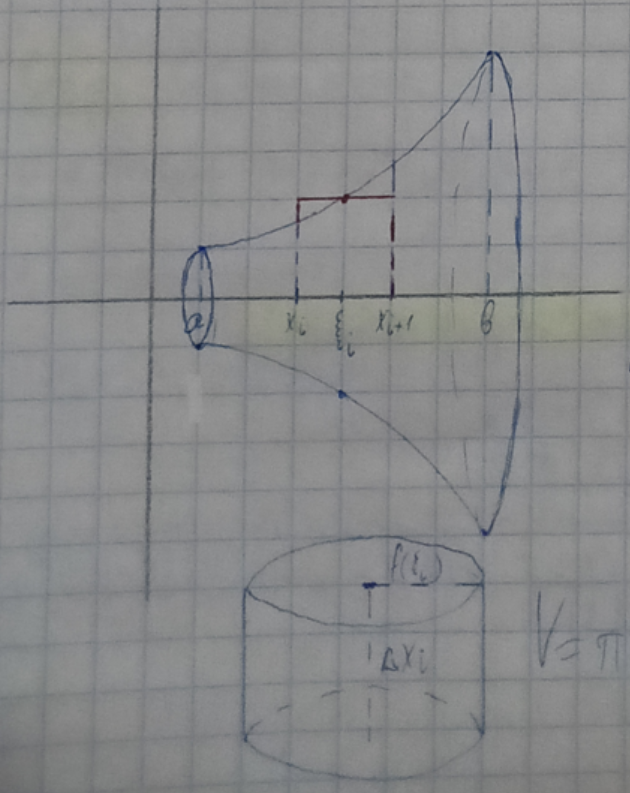
\includegraphics[max size={15cm}{10cm}]{6.11.1.png}
    \end{center}
    \[ R:a=x_0<x_1<\dots<x_n=b \]
    В каждом элементарном $[x_i; x_{i+1}]$ произвольно выберем точку $\xi_i$\\
    Вычислим $f(\xi_i)$. Тогда $V_i=\pi f^2(\xi_i)\Delta x_i$\\
    Составим $\sigma_R$:
    \[ \sigma_R = \sum_{i=0}^{n-1}V_i=\sum_{i=0}^{n-1}\pi f^2(\xi_i)\Delta x_i \]
    \[ \lim_{\lambda_R \to 0}\sigma_R = \boxed {\pi \int_{a}^{b}f^2(x)dx=V_x } \]
    \subsubsection*{Если кривая задана в параметрическом виде:}
    \[ \begin{cases}
        x=x(t)\\
        y=y(t)
    \end{cases} \;\;\; \alpha \leq t \leq \beta \;\;\; x(\alpha)=a \;\;\; x(\beta)=b \]
    \begin{gather*}
        V=\pi \int_{a}^{b}f^2(x)dx =
        \begin{vmatrix}
            x=x(t)\\
            dx=x'(t)dt\\
            x=a \implies t=\alpha\\
            x=a \implies t=\beta
        \end{vmatrix}=
        \boxed{\pi \int_{\alpha}^{\beta} y^2(t)x'(t)dt=V_x}\\
        \boxed{V_y=\pi \int_{c}^{d} x^2(y)dy=\pi \int_{\alpha_1}^{\beta_1} x^2(t)y'(t)dt}
    \end{gather*}
    \subsubsection*{Если кривая задана в полярной системе координат:}\noindent
    Пусть $r=r(\varphi) \;\;\; \alpha \leq \varphi \leq \beta$
    \[ \begin{cases}
        x=rcos(\varphi)=r(\varphi)cos\varphi\\
        y=r(\varphi)sin\varphi
    \end{cases} \]
    \begin{gather*}
        x'(\varphi)=r'cos\varphi-rsin\varphi\\
        \boxed{V_x=\pi \int_{\alpha}^{\beta} r^2(\varphi)sin^2\varphi (r'(\varphi)cos \varphi -r(\varphi)sin\varphi)d\varphi}\\
        \boxed{V_y=\pi \int_{\alpha_1}^{\beta_1}r^2(\varphi)cos^2\varphi(r'(\varphi)sin\varphi + r(\varphi)cos\varphi)d\varphi}
    \end{gather*}

    \subsection{Площадь поверхностей тела вращения}\noindent
    Пусть $f(x) \geq 0 \;\;\; \forall x \in [a;b]$\\
    \begin{center}
        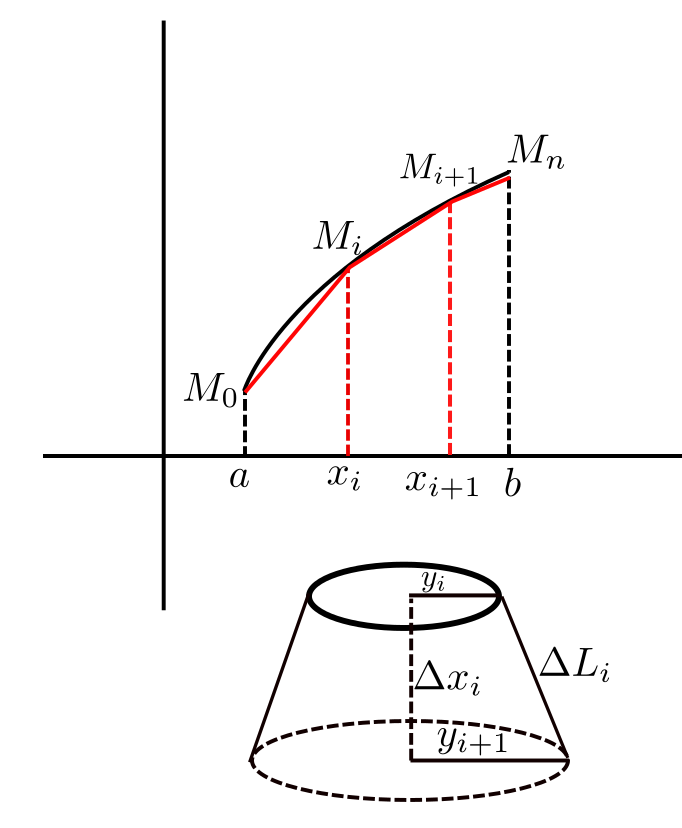
\includegraphics[max size={15cm}{10cm}]{6.12.1.png}
    \end{center}
    \[ R:a=x_0<x_1<x_2<\dots<x_n=b \]
    \[ S_{\text{бок}} = \pi (R + r)l \]
    Обозначим $S_{\text{бок}} = P$.\\
    Обозначим $f(a)=M_0,\dots,f(x_i)=M_i,\dots,f(b)=M_n$\\
    Соединим точки $M_i$ ломаными.
    \[ \Delta l_i = |M_iM_{i=1}| = \sqrt{1+f'(\xi_i)^2}\Delta x_i \; \Delta x_i \]
    $\xi_i$ - произвольная точка $\in [x_i; x_{i+1}]$.
    \[ P_i = \pi(f(x_{i+1}+f(x_i)))\sqrt{1+f'(\xi_i)^2}\Delta x_i \]
    Составим $\sigma_R$:
    \[ \sigma_R = \sum_{i=0}^{n-1}P_i=\sum_{i=0}^{n-1}\pi(f(x_{i+1}+f(x_i)))\sqrt{1+f'(\xi_i)^2 \Delta x_i} \]
    $\sigma_R$ не является интегральной суммой т.к. её значение зависит от $3$-х точек: $\xi_i$, $x_i$, $x_{i+1}$.\\
    Рассмотрим 
    \[ \overline{\sigma_R} = \sum_{i=0}^{n-1} \pi(f(\xi_i)+f(\xi_i))\sqrt{1+f'(\xi_i)^2}\Delta x_i=2\pi \sum_{i=0}^{n-1}f(\xi_i)\sqrt{1+f'(\xi_i)^2}\Delta x_i \]
    $\overline{\sigma_R}$ - интегральная сумма.\\
    Можно показать, что: 
    \[ \forall \delta > 0 \, \exists \, \varepsilon > 0: \lambda_R<\delta \implies |\sigma_R-\overline{\sigma_R}|<\varepsilon \]
    Это значит, что $\lim_{\lambda_R \to 0}\sigma_R=\lim_{\lambda_R \to 0}\overline{\sigma_R}$
    \[ \lim_{\lambda_R \to 0} \sigma_R = \lim_{\lambda_R \to 0} \overline{\sigma_R}= \boxed{2\pi \int_{a}^{b}f(x)\sqrt{1+f'(x)^2}dx = P} \]
    \subsubsection*{Если функция задана в параметрическом виде:}\noindent
    Пусть 
    \[ \begin{cases}
        x=x(t)\\
        y=y(t)
    \end{cases} \;\;\; \alpha \leq t \leq \beta \;\;\; x(\alpha)=a, x(\beta)=b \]
    \[ P_x=\int_{a}^{b}f(x)\sqrt{1+f'(x)^2}dx=\begin{vmatrix}
        x=x(t)\\
        dx=x'(t)dt\\
        x=a \Rightarrow t=\alpha\\
        x=b \Rightarrow t=\beta
    \end{vmatrix}=\boxed{2\pi \int_{\alpha}^{\beta}y(t) \underbrace{\sqrt{x'(t)^2+y'(t)^2}}_{dl}dt} \]
    \[ \boxed{P_y=\int_{\alpha_1}^{\beta_1}x(t)\sqrt{x'(t)^2+y'(t)^2}dt} \]
    \subsubsection*{Если функция задана в полярной системе координат:}\noindent
    Пусть $r=r(\alpha) \;\;\; \alpha \leq \varphi \leq \beta$
    \[ \boxed{P_x=2\pi \int_{\alpha}^{\beta}r(\varphi)sin(\varphi)\sqrt{r^2(\varphi)+r'(\varphi)^2}d\varphi} \]
    \[ \boxed{P_y=2\pi \int_{\alpha_1}^{\beta_1}r(\varphi)cos(\varphi)\sqrt{r^2(\varphi)+r'(\varphi)^2}d\varphi} \]

    \subsection{Физические приложения определенного интеграла}
    \begin{enumerate}
        \item Вычисление рабочей силы\\
        Пусть точка движется вдоль оси $OX$ под действием переменной силы $F(x)$.\\
        Точка перемещается из $x=a$ в $x=b$.
        \begin{center}
            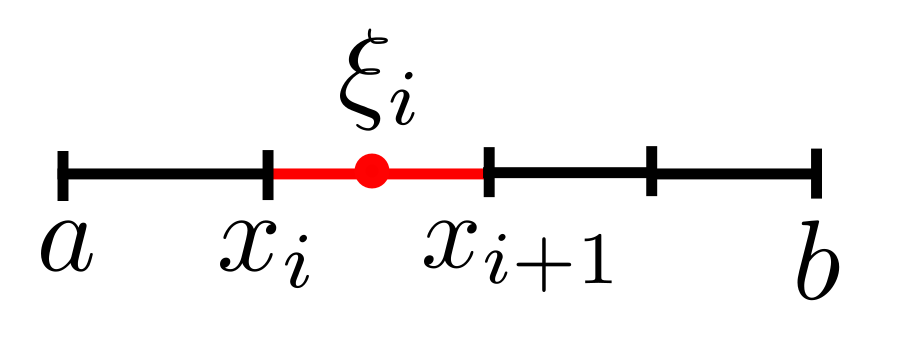
\includegraphics[max size={15cm}{10cm}]{6.13.1.png}
        \end{center}
        \begin{enumerate}
            \item $R: a=x_0<x_1<\dots<x_n=b$
            \item Выберем $\xi_i$
            \item Вычислим $F(\xi_i)$
            \item Составим $\sigma_R=\sum_{i=0}^{n-1}A_i=\sum_{i=0}^{n-1}F(\xi_i)\Delta x_i$
            \[ A=\lim_{\lambda_R \to 0}\sigma_R=\int_{a}^{b}F(x)dx \]
        \end{enumerate}
        \item Центр тяжести кривой и её моменты относительно осей\\
        Рассмотрим $f(x) \geq 0$ на $[a;b]$
        \begin{center}
            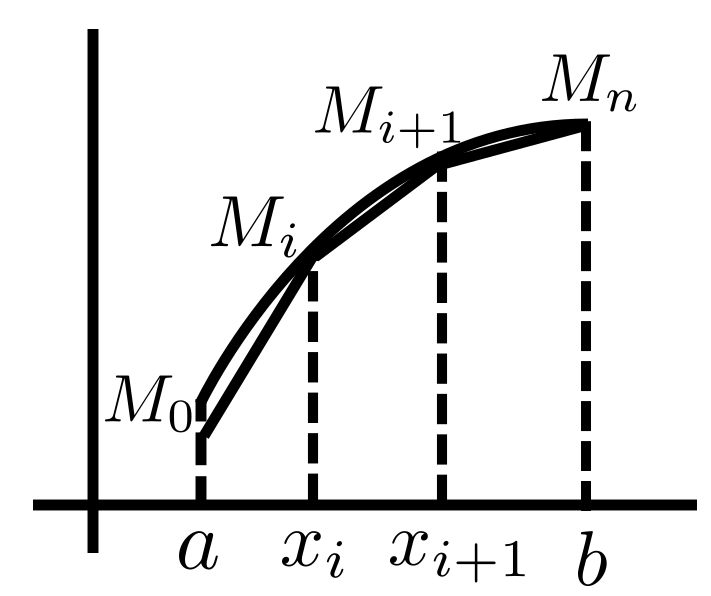
\includegraphics[max size={15cm}{10cm}]{6.13.2.png}
        \end{center}
        $R: a=x_0<x_1<\dots<x_n=b$\\
        Будем рассматривать $M_iM_{i+1}$ - как ломаные, имеющие массу. $\rho =$[кг/м] - линейная плотность.\\
        Составим сумму $\sigma_R$:
        \[ \sigma_R=\sum_{i=0}^{n-1}f(\xi_i)\rho(\xi_i)\Delta L_i=\sum_{i=0}^{n-1} f(\xi_i)\rho(\xi_i)\sqrt{1+f'(\xi_i)^2}\Delta x_i \]
        \[ \lim_{\lambda_R \to 0}\sigma_R=\int_{a}^{b}\underset{r}{f(x)} \underbrace{\rho\sqrt{1+f'(x)^2}}_{m}=M_x \] $M_x$ - момент кривой относительно оси OX.\\
        С другой стороны $(x_0, y_0)$ - центр тяжести кривой.\\
        \[ M_x=my_0 \]
        \begin{gather*}
            my_0=\int_{a}^{b}f(x)\rho(x)\sqrt{1+f'(x)^2}dx\\
            \rho ly_0=\int_{a}^{b}f(x)\rho(x)\sqrt{1+f'(x)^2}dx \;\;\;\;\; \Big| \text{ Пусть } \rho = const\\
            ly_0=\int_{a}^{b}f(x)\sqrt{1+f'(x)^2}dx\\
            l2\pi y_0=2 \pi \int_{a}^{b} f(x)\sqrt{1+f'(x)^2}dx
        \end{gather*}
        \subsubsection*{Теорема 6.13.1 (I-я теорема Гульдена)}\label{th:6.13.1}
        Площадь поверхности, полученной вращением кривой относительно оси $OX$, равна длине этой кривой, умноженной на длину окружности, которую описывает центр тяжести вокруг оси $OX$.\par\noindent
        \underline{Доказательство:}
        \begin{adjustwidth}{1.5em}{1.5em}
            См. выше.
            \[ x_0=\frac{M_y}{m} \;\;\;\;\; y_0=\frac{M_x}{m} \]
            \[ x_0=\frac{\int_{a}^{b}x\rho (x)\sqrt{1+f'(x)^2}dx}{\int_{a}^{b}\underbrace{\rho (x)}_{\rho}\underbrace{\sqrt{1+f'(x)^2}dx}_{dl}} \]
            \[ y_0=\frac{\int_{a}^{b}y\rho (x)\sqrt{1+f'(x)^2}dx}{\int_{a}^{b}\rho (x)\sqrt{1+f'(x)^2}dx} \]
        \end{adjustwidth}
        \item Центр тяжести плоской фигуры и её момент относительно осей:
        \begin{center}
            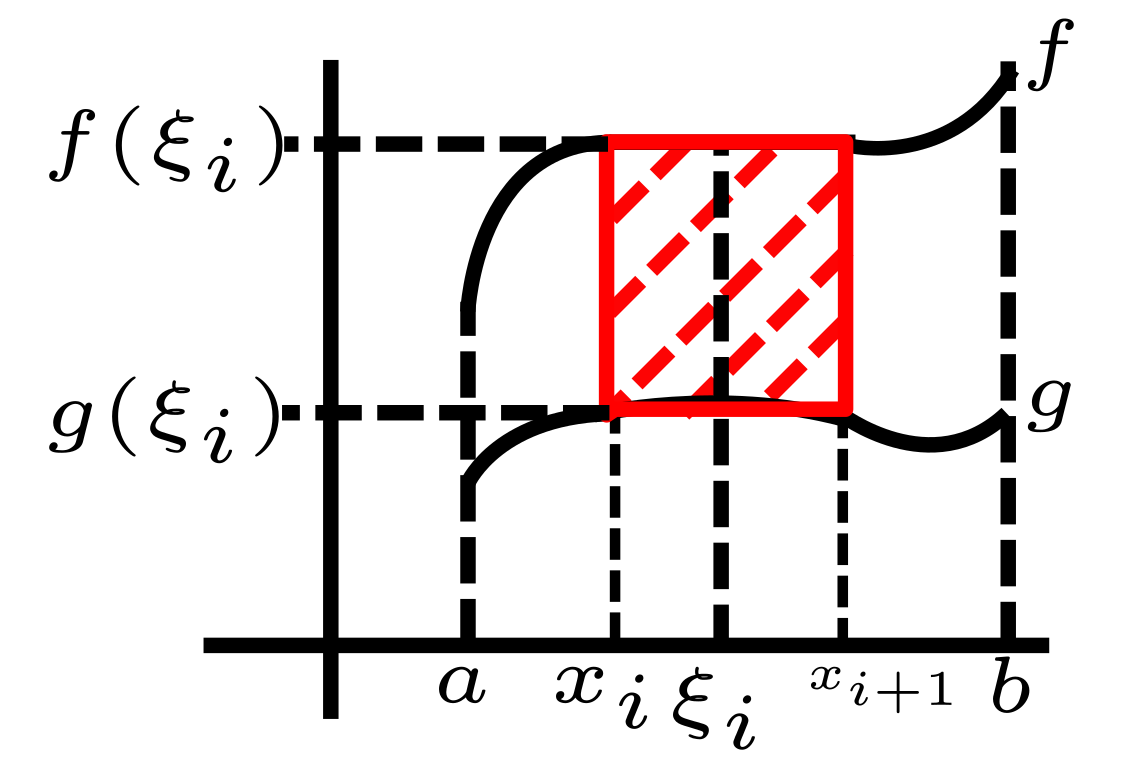
\includegraphics[max size={15cm}{10cm}]{6.13.3.png}
        \end{center}
        Пусть $f(x)\geq 0, g(x)\geq 0 \;\;\; \forall x \in [a;b]$\\
        Пусть $0 \leq g(x) \leq f(x)$\\
        $R:a=x_0<x_1<\dots<x_n=b$\\
        Выберем произвольно точку $\xi_i \in [x_i,x_{i+1}]$\\
        $\rho(\xi_i)=const$\\
        Центр тяжести прямоугольника находится на расстоянии $\frac{1}{2}(f(\xi_i) + g(\xi_i))$\\
        Составим $\sigma_R$:
        \[ \sigma_R=\sum_{i=0}^{n-1}\frac{1}{2} \underbrace{[f(\xi_i)+g(\xi_i)]}_{r_x} \underbrace{\overbrace{\rho(\xi_i)}^{\rho}\overbrace{\overbrace{[f(\xi_i)-g(\xi_i)]}^{\text{высота}}\overbrace{\Delta x_i}^{\text{ширина}}}^{S}}_{m \text{ прямоуг.}} \]
        $[\rho]$ - кг/$\text{м}^2$ - поверхностная плотность.
        \[ \lim_{\lambda_R \to 0} \sigma_R = \int_{R}^{b}\frac{1}{2}\rho (x) [f^2(x)-g^2(x)]dx=M_x \]
        С другой стороны $M_x=my_0$, где $y0$ - $у$-координата центра тяжести.\\
        \begin{gather*}
            my_0=\int_{a}^{b}\frac{1}{2}\rho (x)[f^2(x)-g^2(x)]dx\\
            \rho Sy_0=\int_{a}^{b}\frac{1}{2}\rho (x)[f^2(x)-g^2(x)]dx \;\;\;\;\; \Big| : \rho=const \;\; \Big| \times 2\pi\\
            2S\pi y_0=\pi \int_{a}^{b} [f^2(x)-g^2(x)]dx\\
        \end{gather*}
        \subsubsection*{Теорема 6.13.2 (II-я теорема Гульдена)}\label{th:6.13.2}
        Объём тела, полученного вращением плоской фигуры вокруг оси $OX$, равен площади этой фигуры, умноженной на длину окружности, которую описывает центр тяжести вокруг оси $OX$.\par\noindent
        \begin{gather*}
            y_0=\frac{M_x}{m}=\frac{\frac{1}{2}\int_{a}^{b}\rho (x)[f^2(x)-g^2(x)]dx}{\int_{a}^{b}\rho(x)[f(x)-g(x)]dx}\\
            x_0=\frac{M_y}{m}=\frac{\int_{a}^{b}x\rho (x)[f(x)-g(x)]dx}{\int_{a}^{b}\rho (x)[f(x)-g(x)]dx}
        \end{gather*}
    \end{enumerate}

    \subsection{Несобственные интегралы 1-го рода}\noindent
    Пусть $f(x)$ задана на конечном $[a;b)$.\\
    Допустим, что $f(x)$ интегрируема на $[a;b']$, $b'<b$ и неограниченна в точке $x=b$. Тогда $f(x)$ не интегрируема по Риману на $[a;b]$.\\
    Если $\exists$ конечный $\lim_{b' \to b} \int_{a}^{b'}f(x)dx$, то он называется \textbf{несобственным} интегралом от $f(x)$ на $[a; b]$
    \[ \int_{a}^{b}f(x)dx=\lim_{b' \to b}\int_{a}^{b'} f(x)dx \]
    Если $b=\infty$, т.е. $f(x)$ задана на $[a; +\infty)$ и интегрируема на $\forall [a;A],a<A<\infty$ и $\exists$ конечный $\lim_{A \to \infty}\int_{a}^{A} f(x)dx$, то он называется \textbf{несобственным} интегралом \textbf{1-го рода} от функции $f(x)$ на $[a;+\infty)$.\\
    Аналогично, $\int_{-\infty}^{b}f(x)dx=\lim_{B \to -\infty} \int_{B}^{b}f(x)dx$\\
    \[ \int_{-\infty}^{\infty} f(x)dx=\int_{-\infty}^{C}f(x)dx+\int_{C}^{+\infty}f(x)dx \]

    \subsection{Несобственные интегралы 2-го рода}\noindent
    Пусть $f(x)$ непрерывна $\forall x \in [a;b]/c \;\;\; a \leq c \leq b$\\
    Тогда 
    \[ \int_{a}^{b}f(x)dx=\int_{a}^{c} f(x)dx+\int_{c}^{b} f(x)dx=\lim_{\varepsilon \to 0}\int_{a}^{c-\varepsilon}f(x)dx+\lim_{\varepsilon \to 0}\int_{c+\varepsilon}^{b}f(x)dx \]
    \begin{center}
        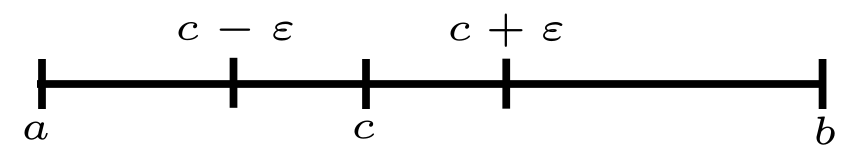
\includegraphics[max size={15cm}{10cm}]{6.15.1.png}
    \end{center}
    Если оба предела $\exists$, то интеграл сходится.\\
    Если хотя бы один $\nexists$ или $\pm \infty$, то расходится.\\
    \underline{Замечание:} точка $c$ может быть $c=a$ или $c=b$.\\
    \underline{Замечание:} можно записать в виде 
    \[ \int_{a}^{b}f(x)dx=\lim_{x \to c-0}\int_{a}^{c}f(x)dx+\lim_{x \to c+0} \int_{c}^{b}f(x)dx \]
    \underline{Пример:}\\
    \begin{enumerate}
        \item Рассмотрим $\int_{1}^{\infty}\frac{dx}{x^k}$
        \begin{enumerate}
            \item $k=1$
            \[ \int_{1}^{\infty}\frac{dx}{x}=\lim_{A \to \infty}\int_{1}^{A} \frac{dx}{x}=\lim_{A \to \infty} \ln |x|\Big|^A_1 = \lim_{A \to \infty}(\ln |A|-\ln 1)=\infty \text{ - расх.} \]
            \item $k \ne 0, k \geq 0$ 
            \begin{gather*}
                \int_{1}^{\infty} \frac{dx}{x^k}=\lim_{A \to \infty}\int_{1}^{A} \frac{dx}{x^k}=\lim_{A \to \infty} (\frac{x^{-k+1}}{-k+1}\Big|^A_1)=\lim_{A \to \infty}
                (\frac{A^{1-k}}{1-k}-\frac{1}{1-k}) =\\
                = \begin{cases}
                    \infty, \;\;\; 0\leq k<1 \text{ - расх.}\\
                    \frac{1}{k-1}, \;\;\; k>1\text{ - сх.}
                \end{cases} 
            \end{gather*}
            \[ \int_{1}^{\infty}\frac{dx}{x^k}=\begin{cases}
                \text{сх. при }k>1\\
                \text{расх. при }k \leq 1
            \end{cases} \]
        \end{enumerate}
        \item $\int_{0}^{1} \frac{dx}{x^k} \;\;\; \varepsilon>0$
        \begin{enumerate}
            \item $k=1$ 
            \[ \int_{0}^{1} \frac{dx}{x}=\lim_{\varepsilon \to 0}\int_{0+\varepsilon}^{1}\frac{dx}{x}=\lim_{\varepsilon \to 0}\ln |x|\Big|^1_\varepsilon =\lim_{\varepsilon \to 0}(\ln 1-\ln |\varepsilon|)=+\infty \text{ - рсх} \]
            \item $k\ne 1$ 
            \[ \int_{0}^{1} \frac{dx}{x^k} = \lim_{\varepsilon \to 0}\int_{\varepsilon}^{1}\frac{dx}{x^k}=\lim_{\varepsilon \to 0}\frac{x^{-k+1}}{-k+1}\Big|^1_\varepsilon =\lim_{\varepsilon \to 0}
            (\frac{1}{1-k}-\frac{\varepsilon^{1-k}}{1-k})=\begin{cases}
                \frac{1}{1-k}, \;\;\; k<1\\
                \infty, \;\;\; k>1
            \end{cases} \]
            \[ \int_{0}^{1}\frac{dx}{x^k} = \begin{cases}
                \frac{1}{1-k}, \;\;\; k<1\\
                \text{расх.}, \;\;\; k\geq 1
            \end{cases} \]
        \end{enumerate}
    \end{enumerate}

    \subsection{Свойство несобственных интегралов}\noindent
    \underline{Замечание:} в точке $x=b$ - особенность
    \begin{enumerate}
        \item Линейность\\
        Если $\int_{a}^{b}f(x)dx$ и $\int_{a}^{b} g(x)dx$ сходятся, то $\int_{a}^{b} [\lambda f(x)+\mu g(x)]dx$ тоже сходится.
        \[ \int_{a}^{b}[\lambda f(x)+\mu g(x)]dx=\lambda \int_{a}^{b} f(x)dx + \mu \int_{a}^{b}g(x)dx \]\noindent
        \underline{Доказательство:}
        \begin{adjustwidth}{1.5em}{1.5em}
            Рассмотрим 
            \begin{gather*}
                \int_{a}^{b}[\lambda f(x)+\mu g(x)]dx=\lim_{\underset{(b' < b)}{b' \to b}} \int_{a}^{b}\left[\lambda f(x)+\mu g(x)\right]dx= \\ \lim_{b' \to b}\left[\lambda \int_{a}^{b'}f(x)dx+\mu \int_{a}^{b'}g(x)dx\right]=
                \lambda\lim_{b' \to b} \int_{a}^{b'}f(x)dx+\mu\lim_{b' \to b}\int_{a}^{b'}g(x)dx=\\ \lambda \int_{a}^{b}f(x)dx+\mu \int_{a}^{b}g(x)dx
            \end{gather*}
            \begin{center}
                \textbf{Ч.т.д.}
            \end{center}
        \end{adjustwidth}
        \item Если $\int_{a}^{b} f(x)dx$ и $\int_{a}^{b} g(x)dx$ сходятся и $\forall x \in [a;b) \;\;\; f(x) \leq g(x)$, то $\int_{a}^{b}f(x)dx \leq \int_{a}^{b}g(x)dx$.\par\noindent
        \underline{Доказательство:}
        \begin{adjustwidth}{1.5em}{1.5em}
            \[ \forall b<b' \; \int_{a}^{b'} f(x) \leq \int_{a}^{b'} g(x)dx \text{ (оценки интервалов)}\]
            Переходя к $\lim_{b' \to b}$ при $b' \to b$, получим \textbf{Ч.т.д.}
        \end{adjustwidth}
        \item Формула замены переменной\\
        Если $f(x)$ непрерывна $\forall x \in [a;b) = \Delta x$, $\varphi(t)$ непрерывно дифференцируема на $\left[\alpha;\underset{\Delta t}{\beta}\right)$ ($\varphi(t)$ непрерывна и $\varphi'(t)$ непрерывна), $\varphi(\Delta t) \subset \Delta x$, $a=\varphi(\alpha)$, $b=\lim_{t \to \beta}\varphi(t)$\\
        Тогда $\int_{a}^{b}f(x)dx=\int_{\alpha}^{\beta} f(\varphi(t))\varphi'(t)dt$.
        \item Формула интегрирования по частям\\
        Если $u(x)$ и $v(x)$ непрерывны на $[a;b)$; $u'(x)$, $v'(x)$ конечно-непрерывны на $[a;b'] \;\;\; a<b'<b$, то $\int_{a}^{b}udv=uv\Big|^b_a - \int_{a}^{b}vdu$
        \[ \int_{a}^{b}udv=\lim_{b' \to b} \left(u(b')v(b')-u(a)v(a)-\int_{a}^{b'}vdu\right) \]
    \end{enumerate}
    \underline{Пример:}
    \begin{gather*}
        \int_{1}^{\infty}\frac{dx}{x\sqrt{x^2-1}}=\lim_{\substack{A \to \infty \\ \varepsilon \to 0}} \int_{1+\varepsilon}^{A} \frac{dx}{x\sqrt{x^2-1}} =
        \begin{vmatrix}
            x=\frac{1}{t} & x=1 \Rightarrow t=1\\
            dx=-\frac{1}{t^2}dt & x=\infty \Rightarrow t=0
        \end{vmatrix} =\\
        = \int_{1}^{0} \frac{-\frac{dt}{t^2}}{\frac{1}{t}\sqrt{\frac{1}{t^2}-1}}=\int_{0}^{1}\frac{dt}{t\sqrt{\frac{1-t^2}{t^2}}} = \int_{0}^{1} \frac{dt}{t\sqrt{\frac{1-t^2}{t^2}}} = \int_{0}^{1}\frac{dt}{\sqrt{1-t^2}} =\\
        = \lim_{\varepsilon \to 0} \int_{0}^{1-\varepsilon}\frac{dt}{\sqrt{1-t^2}}=\lim_{\varepsilon \to 0} \arcsin t\Big|^{1-\varepsilon}_0=\\
        = \lim_{\varepsilon \to 0}[arcsin(1-\varepsilon)-arcsin(0)]=\frac{\pi}{2}
    \end{gather*}

    \subsection{Несобственные интегралы от неотрицательных функций}\noindent
    \textbf{Лемма:} Если $f(x)$ неотрицательна на $[a;b)$, то для сходимости $\int_{a}^{b}f(x)dx \Longleftrightarrow $ чтобы множество интегралов $\int_{a}^{b'} f(x)dx \;\;\; b' \in [a;b)$ было ограничено сверху.\\
    Т.е. чтобы $\exists\,c>0:\forall b':\int_{a}^{b'}f(x)dx \leq \mathbb{C}$\\
    \underline{Доказательство:}
    \begin{adjustwidth}{1.5em}{1.5em}
        Рассмотрим $\varphi(b') = \int_{a}^{b'} f(x)dx$ - функция с переменным верхним пределом.\\
        Пусть $a<b'<b''<b$\\
        Рассмотрим 
        \[ \varphi(b'')=\int_{a}^{b''}f(x)dx = \int_{a}^{b'}f(x)dx+\int_{b'}^{b''}f(x)dx\geq \int_{a}^{b'}f(x)dx=\varphi(b')\]
        Т.е. если $b'<b'' \implies \varphi(b')\leq \varphi(b'')$.\\
        Т.е. $\varphi(b')$ - неубывающая функция.\\
        Существование $\int_{a}^{b}f(x)dx$ означает (по определению) существование конечного предела $\lim_{b' \to b}\varphi(b')=\int_{a}^{b}f(x)dx$, который $\exists$ $\Longleftrightarrow$ когда $\varphi(b')$
        ограничена сверху, т.е. $\varphi(b') \leq \mathbb{C}$.
        \begin{center}
            \textbf{Ч.т.д.}
        \end{center}
    \end{adjustwidth}
    \subsubsection*{Теорема 6.17.1 (1-й признак сравнения несобственных интегралов)}\label{th:6.17.1}\noindent
    Пусть $0\leq g(x) \leq f(x) \;\;\; x\in [a;b)$\\
    Тогда
    \begin{enumerate}
        \item Если $\int_{a}^{b}f(x)dx$ сх. $\implies \int_{a}^{b}g(x)dx$ сх.
        \item Если $\int_{a}^{b}g(x)dx$ расх. $\implies \int_{a}^{b}f(x)dx$ расх.
    \end{enumerate}
    \underline{Доказательство:}
    \begin{adjustwidth}{1.5em}{1.5em}
        \begin{enumerate}
            \item Пусть $\int_{a}^{b}f(x)dx$ сх., тогда множество интегралов $\int_{a}^{b'}f(x)dx$ по лемме ограничены сверху.\\
            Т.к. $g(x) \leq f(x) \implies \int_{a}^{b'}g(x)dx \leq \int_{a}^{b'}f(x)dx \implies \forall b' \in (a;b)$ множество интегралов $\int_{a}^{b'}g(x)dx$ будут ограничены сверху $\implies$ по лемме $\int_{a}^{b}g(x)dx$ сх.
            \item Пусть $\int_{a}^{b}g(x)dx$ расх., тогда $\int_{a}^{b}f(x)dx$ не может сходится, т.к. если бы они сх., то $\int_{a}^{b}g(x)dx$ тоже сх. по пункту 1, а это не так.
        \end{enumerate}
        \begin{center}
            \textbf{Ч.т.д.}
        \end{center}
    \end{adjustwidth}
    \subsubsection*{Теорема 6.17.2 (следствие 1-го признака сравнения или 2-й признак сравнения)}\label{th:}
    Пусть $\forall x \in [a;b) \;\;\; f(x)\geq 0,g(x)\geq 0$ и $\lim_{x \to b}\frac{f(x)}{g(x)}=k$
    \begin{enumerate}
        \item Если $\int_{a}^{b}g(x)dx$ - сх., $0\leq k< \infty$ - конечное $\implies \int_{a}^{b}f(x)dx$ сх.
        \item Если $\int_{a}^{b}g(x)dx$ - расх., $0 < k \leq \infty \implies \int_{a}^{b}f(x)dx$ - расх.
    \end{enumerate}
    \underline{Доказательство:}
    \begin{adjustwidth}{1.5em}{1.5em}
        \begin{enumerate}
            \item Пусть $0\leq k < \infty$\\
            Т.к. $\lim_{x \to b} \frac{f(x)}{g(x)} = k$, то $\exists\,b' \in [a;b):\forall x\in (b';b) \; \frac{f(x)}{g(x)}<{k+1}$\\
            $\int_{a}^{b}g(x)dx$ - сх. $\implies \int_{b}^{b}g(x)dx$ - сх. $\implies \int_{b'}^{b}(k+1)g(x)dx$ - сх. $\implies \int_{b'}^{b}f(x)dx$ сх. по признаку сравнения $\implies \int_{a}^{b}f(x)dx$ сх.
            \item Пусть $0<k\leq \infty$. Пусть $0<k'<k$.\\
            $\int_{a}^{b}g(x)dx$ - расх. Тогда $\forall x \in (b';b) \; \frac{f(x)}{g(x)}>k'$\\
            $f(x)>k'g(x)$\\
            $\int_{a}^{b}g(x)dx$ расх. $\implies \int_{b'}^{b} g(x)dx$ расх. $\implies \int_{b'}^{b} k'g(x)dx$ расх. $\implies \int_{b'}^{b}f(x)dx$ по признаку
            сравнения $\implies \int_{a}^{b}f(x)dx$ расх. 
            \begin{center}
                \textbf{Ч.т.д.}
            \end{center}
        \end{enumerate}
    \end{adjustwidth}
    \underline{Пример:}
    \begin{adjustwidth}{1.5em}{1.5em}
        $\int_{0}^{1} \ln(x)dx$\\
        Пусть $f(x)=\ln(x)$\\
        $g(x)=\frac{1}{x^2} \;\;\; \int_{0}^{1}\frac{dx}{x^2}$ - расх.\\
        \[ \lim_{x \to 0}\frac{\ln(x)}{\frac{1}{x^2}}=\lim_{x \to 0}\frac{\frac{1}{x}}{-\frac{2}{x^3}}=\lim_{x \to 0}\frac{x^2}{-2}=0 \]
        \[ g(x)=\frac{1}{\sqrt{x}} \;\;\; \int_{0}^{1}=\frac{dx}{\sqrt{x}} \text{ - сх.}\]
        Рассмотрим 
        \[ \lim_{x \to 0}\frac{\ln(x)}{\frac{1}{\sqrt{x}}}=\lim_{x \to 0}\frac{\frac{1}{x}}{-\frac{1}{2x^{\frac{3}{2}}}}=\lim_{x \to 0}(-2\sqrt{x})=0 \implies \int_{0}^{1}\ln(x)dx \text{ - сх.}\]
    \end{adjustwidth}

    \subsection{Критерий Коши сходимости несобственных интегралов. Абсолютно сходящиеся интегралы.}
    \subsubsection*{Теорема 6.18.1}\label{th:6.18.1}
    $\int_{a}^{b}f(x)dx$ сх. $\Longleftrightarrow$ когда $\forall \varepsilon > 0\,\exists\,a<b_0<b:\forall b',b'':b_0<b'<b''<b$
    \[ \left| \int_{b'}^{b''}f(x)dx \right| < \varepsilon \]
    \underline{Доказательство:}
    \begin{adjustwidth}{1.5em}{1.5em}
        Рассмотрим $\varphi(b_0)=\int_{a}^{b_0}f(x)dx$ - функция с переменным верхним пределом.\\
        Существование $\int_{a}^{b}f(x)dx$ означает существование $\lim_{b_0 \to b}\varphi(b_0)$\\
        $\lim_{b_0 \to b}\varphi(b_0)$ $\exists \Longleftrightarrow$ когда $\exists$ окрестность точки $b$: $\forall b',b'' \in $ окружности выполняется $|b''-b'|<\delta \implies |\varphi(b'')-\varphi(b')|<\varepsilon$\\
        А это означает $\left| \int_{a}^{b''}f(x)dx - \int_{a}^{b'}f(x)dx \right| < \varepsilon \implies \left| \int_{b'}^{b''} f(x)dx \right| < \varepsilon$
        \begin{center}
            \textbf{Ч.т.д.}
        \end{center}
    \end{adjustwidth}
    Пусть $f(x)$ задана на $[a;b)$ и интегрируема по Риману $\forall\,[a;b'] \;\;\; a<b'<b$\\
    $\int_{a}^{b}f(x)dx$ называется \textbf{абсолютно сходящимся}, если сходятся $\int_{a}^{b}|f(x)|dx$.
    \subsubsection*{Теорема 6.18.2 (критерий Коши абсолютной сходимости несобственных интегралов)}\label{th:6.18.2}
    Для того, чтобы $\int_{a}^{b}f(x)dx$ абсолютно сх. $\Longleftrightarrow$ 
    \[ \forall \varepsilon >0\,\exists\,b_0:a<b_0<b: \forall b',b'':\\b_0<b'<b''<b \implies \left|\int_{b'}^{b''}|f(x)|dx\right| < \varepsilon \]
    \underline{Доказательство:}
    \begin{adjustwidth}{1.5em}{1.5em}
        Следует из критерия Коши для интеграла $\int_{a}^{b}|f(x)|dx$
        \begin{center}
            \textbf{Ч.т.д.}
        \end{center}
    \end{adjustwidth}
    \subsubsection*{Теорема 6.18.3}\label{th:6.18.3}
    Если несобственный интеграл абсолютно сходится, то он сходится.\par\noindent
    \underline{Доказательство:}
    \begin{adjustwidth}{1.5em}{1.5em}
        $\int_{a}^{b}|f(x)|dx$ сходится, тогда по критерию Коши на $(a;b)$ $\exists\,b_0:b_0<b'<b''<b \implies \left|\int_{b'}^{b''}|f(x)|dx\right|< \varepsilon$\\
        Рассмотрим $\left|\int_{b'}^{b''}f(x)dx\right|\leq \left|\int_{b'}^{b''}|f(x)|dx\right|<\varepsilon$\\
        Т.е. выполняется критерий Коши сходимости интеграла $\int_{a}^{b}f(x)dx$
        \begin{center}
            \textbf{Ч.т.д.}
        \end{center}
    \end{adjustwidth}
    \textbf{Свойство:} Если $\int_{a}^{b}f(x)dx$ абсолютно сходится, $g(x)$ интегрируема по Риману $\forall\,[a;b'] \subset [a;b)$ и ограничена на $[a;b)$, то $\int_{a}^{b}f(x)g(x)dx$ сх.\par\noindent
    \underline{Доказательство:}
    \begin{adjustwidth}{1.5em}{1.5em}
        $\int_{a}^{b'}f(x)dx \;\; \exists$ по условию, $\int_{a}^{b'}g(x)dx \;\; \exists$ по условию $\implies \int_{a}^{b'}f(x)g(x)dx \;\; \exists$ (по свойству).\\
        Рассмотрим $\int_{a}^{b}|f(x)g(x)|dx \leq \underbrace{c\int_{a}^{b}|f(x)|dx}_{\text{абс. сх. по условию}}$\\
        Тогда $\int_{a}^{b}|f(x)g(x)|dx$ сх, по 1-му признаку сравнения.\\
        Тогда $\int_{a}^{b}f(x)g(x)dx$ сх. абсолютно по Опр.
    \end{adjustwidth}
    \begin{center}
        \textbf{Ч.т.д.}
    \end{center}

    \subsection{Признаки сходимости Дирихле́ и Абеля несобственных интегралов 1-го рода}
    \subsubsection*{Теорема 6.19.1 Признак Дирихле́}\label{th:6.19.1}
    Если на полуоси $x\geq a$
    \begin{enumerate}
        \item $f(x)$ непрерывна и имеет ограниченную первообразную на $x\geq a$
        \item $g(x)$ непрерывно дифференцируема и убывает при этом $\lim_{x \to \infty}g(x)=0$
    \end{enumerate}
    Тогда $\int_{a}^{\infty}f(x)g(x)dx$ сх.\\
    \underline{Доказательство:}
    \begin{adjustwidth}{1.5em}{1.5em}
        Пусть $F(x)$ - ограниченная первообразная $f(x)$ на $x \geq a$\\
        Рассмотрим 
        \begin{gather*}
            \int_{a}^{b}f(x)g(x)dx=\int_{a}^{b}\underbrace{g(x)}_{u} \underbrace{d(F(x))}_{du}=g(x)F(x)\Big|^b_a-\int_{a}^{b}F(x)g'(x)dx =\\
            = \underbrace{g(b)F(b)}_{\to 0}-\underbrace{g(a)F(a)}_{\text{const}}-\int_{a}^{b}F(x)g'(x)dx
        \end{gather*}
        Рассмотрим $\lim_{b \to \infty}\underbrace{g(b)}_{\to 0} \underbrace{F(b)}_{\text{огр.}}=0$. Докажем, что $\int_{a}^{\infty}F(x)g'(x)dx$ сх.\\
        Рассмотрим 
        \begin{gather*}
            \int_{a}^{b}|F(x)g'(x)|dx=-\int_{a}^{b}|F(x)|g'(x)dx \leq -c \int_{a}^{b}g'(x)dx=-c g(x)\Big|^b_a =\\
            = c(g(a)-g(b))\leq cg(a) \text{ - const}
        \end{gather*}
        Получим, что множество интегралов $\int_{a}^{b}|F(x)g'(x)|dx$ ограничены сверху $\implies \int_{a}^{\infty}|F(x)g'(x)|dx$ сх. (по лемме из 6.17) $\implies \int_{a}^{\infty}F(x)g'(x)dx$ абсолютно сх. по определению $\implies$ сх. (\hyperref[th:6.18.3]{теорема 6.18.3})\\
        Тогда $\int_{a}^{\infty}f(x)g(x)dx$ сходится.
        \begin{center}
            \textbf{Ч.т.д.}
        \end{center}
    \end{adjustwidth}
    \subsubsection*{Теорема 6.19.2 (признак Абеля)}\label{th:6.19.2}
    Если на $x\geq a$
    \begin{enumerate}
        \item $f(x)$ непрерывна на $x \geq a$ и $\int_{a}^{\infty}f(x)dx$ сх.
        \item $g(x)$ непрерывно дифференцируема, ограниченна и монотонна.
    \end{enumerate}
    Тогда $\int_{a}^{\infty}f(x)g(x)dx$ сх.\par\noindent
    \underline{Доказательство:}
    \begin{adjustwidth}{1.5em}{1.5em}
        \underline{Замечание:} $\int_{a}^{\infty}f(x)g(x)dx$ и $\int_{a}^{\infty}f(x)(-g(x))dx$ сх. или расх. одновременно. Тогда одна из функция $g(x)$ или $(-g(x))$ будет убывающей (невозрастающей).\\
        Пусть для определённости $g(x)$ убывает.\\
        По условию $\lim_{x \to \infty}g(x) = \mathbb{C}$\\
        Т.е. $\lim_{x \to \infty}(g(x) - \mathbb{C}) = 0$\\
        Рассмотрим 
        \[ f(x)g(x) = f(x)g(x)-cf(x)+cf(x)=f(x)[g(x)-c]+cf(x) \]
        Надо показать, что $\int_{a}^{\infty}f(x)[g(x)-c]dx$ сх. и $\int_{a}^{\infty}cf(x)dx$ сх.\\
        $c\int_{a}^{\infty}f(x)dx$ сх. по условию.\\
        Рассмотрим 
        \[ \int_{a}^{\infty}f(x)dx=\int_{a}^{\infty}f(t)dt= \underbrace{\lim_{x \to \infty}\int_{a}^{x}f(t)dt}_{F(x)} =\lim_{x \to \infty}F(x)\]
        $\int_{a}^{\infty}f(x)dx$ сх. $\implies \lim_{x \to \infty}F(x) \;\; \exists \implies F(x)$ ограничена в окрестности бесконечно удалённой точки.\\
        $F(x)$ - первообразная для $f(x)$ на $x \leq a$\\
        Рассмотрим 
        \[ \int_{a}^{\infty} \underbrace{f(x)}_{\substack{\text{непр.}\\\text{имеет огр. первообр.}}} \underbrace{[g(x)-c]}_{\substack{\text{непр.}\\\text{дифф-ма}\\\text{убыв. и стр. к 0}}}dx\] 
        Тогда интеграл сходится по признаку Дирихле́.\\
        Т.е. $\int_{a}^{\infty}f(x)g(x)dx$ сх.
        \begin{center}
            \textbf{Ч.т.д.}
        \end{center}
    \end{adjustwidth}
    \underline{Примеры:}\\
    \begin{enumerate}
        \item $\int_{1}^{\infty}\frac{\sin(x)}{x^\alpha}dx \;\;\; \alpha>0$\\
        $f(x) = \sin x$ (непр., имеет огр. первообр.)\\
        $g(x)=\frac{1}{x^\alpha}$ (непр., диф-ма, $\lim_{x \to \infty}\frac{1}{x^\alpha}=0$, убывает)\\
        Интеграл сходится по признаку Дирихле́
        \item $\int_{1}^{\infty}\frac{\sin x \arctg x}{x^\alpha}dx \;\;\; \alpha>0$\\
        $f(x)=\frac{\sin x}{x^\alpha}$ (непр. и $\int_{1}^{\infty}\frac{\sin x}{x^\alpha}$ сх.)\\
        $g(x)=\arctg x$ (непр., дифф-ма, огр., возрастает)\\
        Тогда $\int_{1}^{\infty}\frac{\sin x \arctg x}{x^\alpha}dx$ сх. по признаку Абеля.
    \end{enumerate}



    \section{Функции нескольких переменных}
    \subsection{Основные понятия}\noindent
    Рассмотрим упорядоченное множество $E$ пар чисел $(x; y)$\\
    Пары $(x_1; y_1)$ и $(x_2; y_2)$ равны $\Longleftrightarrow$ $x_1 = x_2, y_1 = y_2$.\par\noindent
    Пусть каждой паре $(x; y) \in E$ по некоторому закону ставится в соответствие единственное число $z$. Тогда говорят, что на $E$ определена \textbf{функция} $z = f(x; y)$.\\
    \underline{Примеры:}
    \begin{center}
        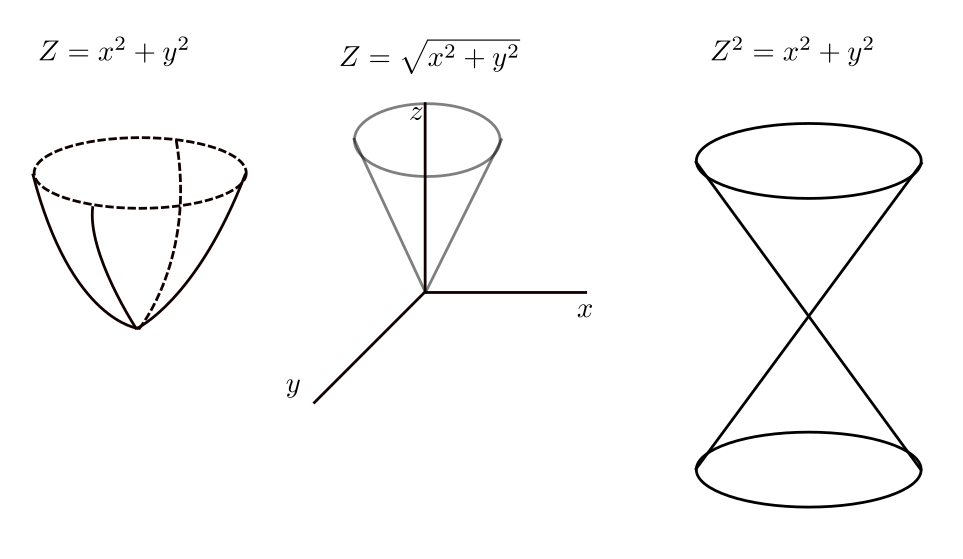
\includegraphics[max size={15cm}{10cm}]{7.1.1.png}
    \end{center}
    Рассмотрим множество упорядоченных систем
    \[ (x_1, x_2, \dots, x_n), n \in N \]
    Элементы этого множества можно рассматривать как точку $n$-мерного пространства $R^n$, а можно как $n$-мерные векторы.\\
    В первом случае для них вводится понятие расстояния, во втором случае - соответствующие векторные операции.\par\noindent
    \textbf{В случае вектора:}
    \begin{align*}
        \text{Пусть }&\overline{x} (x_1, \dots, x_n)\\
        &\overline{y}(y_1,\dots,y_n)
    \end{align*}
    \begin{gather*}
        \lambda\overline{x} + \mu \overline{y} = (\lambda x_1 + \mu y_1; \lambda x_2 + \mu y_2; \dots; \lambda x_n + \mu y_n)\\
        \overline{x}\overline{y} = x_1y_1 + \dots + x_ny_n
    \end{gather*}
    Множество всех упорядоченных систем $\overline{x} = (x_1, \dots, x_n)$, для которых определены линейная комбинация и скалярное произведение двух элементов называется \textbf{$n$-мерным арифметическим Евклидовым пространством}.\par\noindent
    \textbf{В случае точки:}
    \begin{gather*}
        \rho (x,y) \text{ - расстояние между точками}\\
        \rho (x,y) = |x - y| = \sqrt{ \sum_{i = 1}^{n} (x_i - y_i)^2 }
    \end{gather*}
    Множество точек $x = (x_1, \dots, x_n)$, для которых выполняется неравенство $\rho (x, x^0) < \varepsilon$, называется \textbf{$\varepsilon$-окрестностью} точки $x^0$.\\
    Точки множества называется \textbf{внутренними} точками, если $\exists$ $\varepsilon$-окрестность, целиком содержащаяся в этом множестве.\\
    Точки множества называется \textbf{граничными} точками, если $\forall$ её $\varepsilon$-окрестность содержит как внутренние, так и внешние точки.\\
    Точки множества называется \textbf{внешними} точками, если $\exists$ $\varepsilon$-окрестность, не содержащая ни одной точки множества.\par\noindent
    Пусть в $R^n$
    \begin{center}
        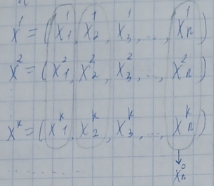
\includegraphics[max size={15cm}{10cm}]{7.1.2.png}
    \end{center}
    Т.е. в пространстве $R^n$ задана последовательность $\{x^k\}$.\\
    Точка $x^0 = (x^0_1, x^0_2, x^0_3, \dots, x^0_n)$ называется \textbf{пределом} последовательности $\{x^k\}$, если $\lim_{k\to\infty} \rho(x^k, x^0) = 0$\\
    \underline{Обозначение:} $\lim_{k\to\infty}x^k=x^0$\\
    \underline{Или}: Точка $x^0 = (x^0_1, x^0_2, x^0_3, \dots, x^0_n)$ называется \textbf{пределом} последовательности $\{x^k\}$, если $\forall \varepsilon > 0$ $\exists \text{ } n_0 \text{ } \big| \text{ } \forall n > n_0 : \rho(x^n, x^0) < \varepsilon$\\
    Определение $\lim_{k\to\infty}x^k=x^0$ эквивалентно $n$ одномерным пределам.
    \[ \lim_{k\to\infty}x^k_1 = x^0_1; \lim_{k\to\infty}x^k_2 = x^0_2; \dots; \lim_{k\to\infty}x^k_n = x^0_n \]

    \subsection{Предел функций нескольких переменных в точке}
    \noindent Пусть функция $f(x_1, \dots, x_n)$ определена в $u(x^0)$, быть может за исключением самой точки $x^0$.\\
    \textbf{По Гейне:} точка $a$ (одномерное число) называется \textbf{пределом функции} $f$ \textbf{в точке} $x^0$ ($f(x_1, \dots, x_n)$), если $\forall$ последовательности $\{x^k\} : \lim_{k\to\infty}x^k=x^0$, числовая последовательность $\{ f(x^k) \}$ (одномерная) имеет своим пределом точку $a$ ($\lim_{k\to x^0}f(x)=a$).\par\noindent
    \textbf{По Коши:} точка $a$ называется \textbf{пределом функции} $f(x_1, \dots, x_n)$ \textbf{в точке} $x^0$, если
    \[ \forall \varepsilon > 0 \text{ } \exists \text{ } \delta = \delta(\varepsilon) > 0 : \rho(x, x^0) < \delta \implies |f(x_1, \dots, x_n) - a| < \varepsilon \]
    Рассмотрим функцию $f(x,y)$, заданную в окрестности точки $(x_0; y_0)$
    \begin{adjustwidth}{1.5em}{1.5em}
        Пусть $\overline{\omega} (\omega_x, \omega_y)$ - единичный вектор.\\
        $\frac{x - x_0}{\omega_x} = \frac{y - y_0}{\omega_y}$ - уравнение прямой, проходящей через точку $(x_0; y_0)$ с направляющим вектором $\overline{\omega}$.
        \[ \begin{cases}
            x = \omega_xt + x_0\\
            y = \omega_yt + y_0
        \end{cases}\text{ - параметрическое уравнение прямой} \]
        Пусть $t \ge 0$. Получим луч, выходящий из точки $(x_0; y_0)$ в направлении $\overline{\omega}$.
        \begin{center}
            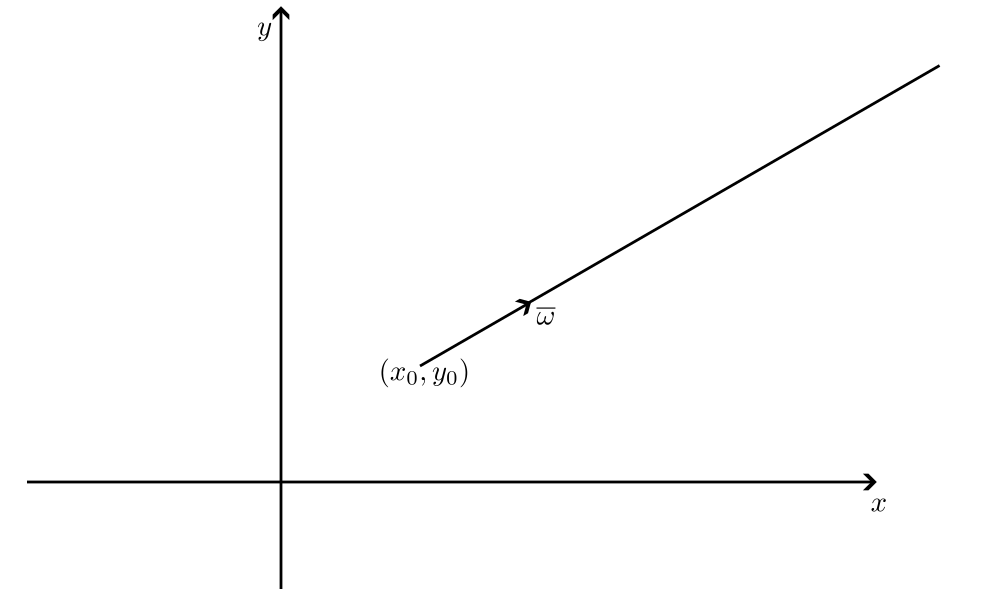
\includegraphics[max size={15cm}{10cm}]{7.2.1.png}
        \end{center}
    \end{adjustwidth}\noindent
    Рассмотрим $\underbrace{f(x; y)}_{\text{ф. 2-х перем. x, y}} = \underbrace{f(x_0+\omega_xt; y_0+\omega_yt)}_{\text{ф. 1 перем. t}}$.
    $\lim_{t \to 0} f(x_0+\omega_xt; y_0+\omega_yt)$, если он $\exists$, называется \textbf{пределом функции} $f(x, y)$ \textbf{в точке} $(x_0; y_0)$ \textbf{по направлению} $\overline{\omega}$.\\
    \underline{Пример:}
    \begin{adjustwidth}{1.5em}{1.5em}
        Рассмотрим $f(x,y) = \frac{x^2y}{x^4 + y^2}$; $f(x,y)$ определена $\forall x, y \in R$, кроме точки $(0, 0)$.
        \[ \lim_{x \to 0\,y \to 0} \frac{x^2y}{x^4 + y^2} = \left[ \frac{0}{0} \right] = \begin{vmatrix}
            y = kx\\
            x \to 0 \Rightarrow y \to 0
        \end{vmatrix} = \lim_{x\to 0} \frac{kx^3}{x^4+k^2x^2} = \lim_{x \to 0}\frac{kx}{x^2+k^2} = 0 \]
        Проверим, может ли быть несовпадение пределов при другом значении $y$.
        \[ \lim_{x \to 0\,y \to 0} \frac{x^2y}{x^4 + y^2} = \begin{vmatrix}
            y = x^2\\
            x \to 0 \Rightarrow y \to 0
        \end{vmatrix} = \lim_{x \to 0}\frac{x^4}{x^4+x^4} = \frac{1}{2} \]
        Пределы не совпали $\Rightarrow$ предел $\nexists$.
    \end{adjustwidth}
    Определение:
    \begin{align*}
        &\lim_{x \to x_0\, y \to y_0}f(x;y)=\infty & &\forall M > 0\, \exists\, \delta = \delta(M): \rho(\underset{M(x,y)}{M}, \underset{M_0(x_0, y_0)}{M_0}) < \delta \Rightarrow |f(x;y)| > M\\
        &\lim_{x\to\infty\, y\to\infty}f(x,y) = a & &\forall \varepsilon > 0\, \exists\, K = K(\varepsilon): |x| > K, |y| > K \Rightarrow |f(x,y) - a| < \varepsilon\\
        &\lim_{x\to-\infty\, y\to y_0}f(x,y) = -\infty & &\forall M > 0\, \exists\, \delta = \delta(M): x < -\frac{1}{\delta}, |y-y_0|<\delta \Rightarrow f(x,y) < -M
    \end{align*}

    \subsection{Непрерывность функций нескольких переменных.}\noindent
    Функция $f(x_1, \dots, x_n)$ называется \textbf{непрерывной} в точке $x^0 = (x^0_1, x^0_2, \dots, x^0_n)$, если она определена в некоторой окрестности точки $x^0$, в том числе и в самой точке $x^0$ и $\lim_{x \to x_0} f(x) = f(x^0)$ при $x = (x_1, \dots, x_n)$, $x^0 = (x^0_1, \dots, x^0_n)$.\par\noindent
    \textbf{В эквивалентной форме:}
    \begin{enumerate}
        \item \[ \lim_{\Delta x_i \to 0} f(x^0_1 + \Delta x_1; x^0_2 + \Delta x_2; \dots; x^0_n + \Delta x_n) = f(x^0_1; x^0_2; \dots; x^0_n) \]
        \item Пусть $\Delta f = f(x_1 + \Delta x_1; x_2 + \Delta x_2; \dots; x_n + \Delta x_n) - f(x_1; x_2; \dots; x_n)$ - приращение $f$.\\
        $f(x_1; \dots; x_n)$ непрерывна в точке $x^0$, если $\lim_{\Delta x_i \to 0}\Delta f = 0$.
    \end{enumerate}
    \underline{Замечание:} сумма, разность, произведение и частное непрерывных функций в точке так же являются непрерывной функцией в точке.\par\noindent
    \underline{Замечание:} функции
    \[ \begin{cases}
        x_1 = \varphi_1(t)\\
        x_2 = \varphi_2(t)\\
        \vdots\\
        x_n = \varphi_n(t)
    \end{cases} \]
    $a \le t \le b$, непрерывные на $[a;b]$, определяют непрерывную кривую в $R^n$, соединяющую точки $x^1 = (\varphi_1(a); \varphi_2(a); \dots; \varphi_n(a))$ и $x^2 = (\varphi_1(b); \varphi_2(b); \dots; \varphi_n(b))$, где $t$ - параметр кривой.\\
    Множество $G$ называется \textbf{связным}, если $\forall$ его две точки можно соединить непрерывной кривой, целиком лежащей в $G$.
    
    \subsection{Частные производные функций нескольких переменных.}
    \[ f'(x) = \frac{df}{dx} = \lim_{\Delta x \to 0}\frac{f(x+\Delta x) - f(x)}{\Delta x} \]
    Пусть функция $f(x_1, \dots, x_n)$ определена в некоторой окрестности точки $x^0 = (x^0_1, x^0_2, \dots, x^0_n)$\\
    $\Delta x_k f = f(x_1, x_2, \dots, x_k + \Delta x_k, \dots, x_n) - f(x_1, x_2, \dots, x_k, \dots, x_n)$ - частное приращение функции по переменной $x_k$.
    \[ \lim_{\Delta x_k \to 0} \frac{\Delta x_k f}{\Delta x_k} = \frac{\partial f}{\partial x_k} = f'_{x_k} \]
    Т.е. частная производная по переменной $x_k$ - это обычная производная по этой переменной при условии, что все остальные фиксированные.\\
    \underline{Пример:}
    \[ f(x,y) = x^y \]
    \[ \frac{\partial f}{\partial x} = yx^{y-1} \]
    \[ \frac{\partial f}{\partial y} = x^y \ln x \]
    \underline{Замечание (\textbf{!!!}):} из существования у функции всех частных производных \textbf{НЕ} следует непрерывность этой функции в рассматриваемой точке (в отличие от функции одной переменной).
    \begin{center}
        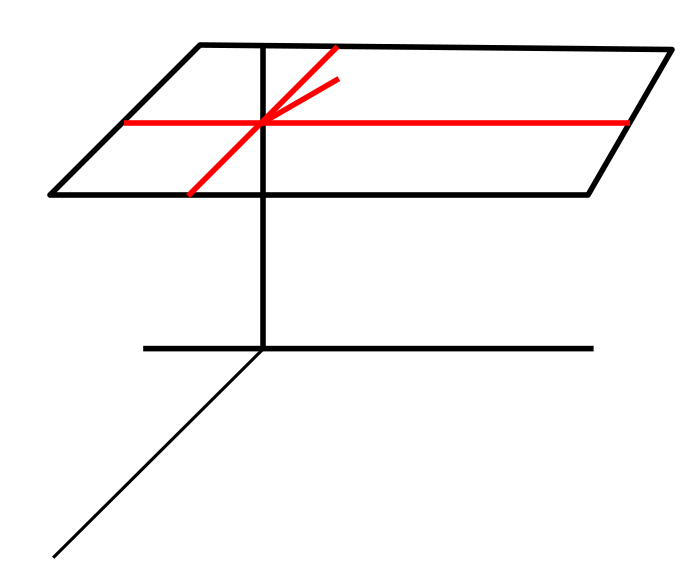
\includegraphics[max size={15cm}{10cm}]{7.4.1.png}
    \end{center}
    \begin{gather*}
        f(x, y) = \begin{cases}
            0, xy = 0\\
            1, xy \ne 0
        \end{cases}\\
        \frac{\partial f}{\partial x} \Big|_{(0; 0)} = \frac{\partial f}{\partial y} \Big|_{(0; 0)} = 0\\
        \text{Но } f \text{ не является непрерывной в точке } (0; 0)\\
        \lim_{x\to 0\, y\to 0}f(x,y) = | y = x | = 1 \ne f(0;0) = 0
    \end{gather*}

    \subsection{Дифференцируемость функций нескольких переменных.}\noindent
    Пусть функция $z = f(x;y)$ определена в некоторой окрестности точки $M_0 = u(M_0, \delta)$.\\
    Пусть точка $M (x; y) \in u(M_0; \delta)$.
    \begin{center}
        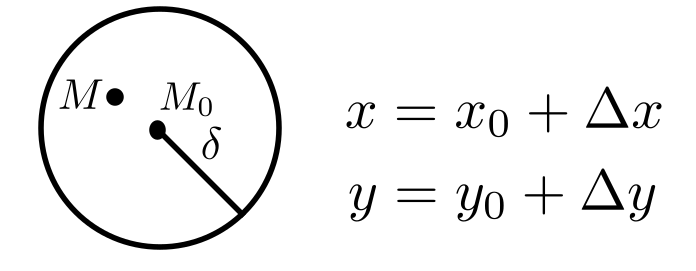
\includegraphics[max size={15cm}{10cm}]{7.5.1.png}
    \end{center}
    Функция $z = f(x;y)$ называется \textbf{дифференцируемой} в точке $M_0 (x_0; y_0)$, если существуют конечные $A$ и $B$ такие, что приращение $\Delta z$ в окрестности точки $M_0$ представимо в виде
    \[ \Delta z = A \Delta x + B \Delta y + o(\rho), \rho \to 0, \rho = \sqrt{\Delta x^2 + \Delta y^2} \]
    \underline{Замечание:} рассмотрим $\varepsilon = \varepsilon (\Delta x; \Delta y): \lim_{\rho \to 0}\varepsilon = 0$. Тогда $o(\rho) = \underset{\text{б. малое}}{\varepsilon(\Delta x; \Delta y)} \times \underset{\text{б. малое}}{\rho}$. Тогда
    \[ \Delta z = A \Delta x + B \Delta y + \varepsilon (\Delta x; \Delta y) \times \rho \]
    Если $z = f(x; y)$ дифференцируема в точке $(x_0; y_0)$, то линейная часть приращения $\Delta z = A \Delta x + B \Delta y$ называется \textbf{дифференциалом} функции $z$ в точке $(x_0; y_0)$.
    \begin{gather*}
        \Delta x = dx, \Delta y = dy\\
        \Delta z = Adx + Bdy
    \end{gather*}
    \subsubsection*{Теорема 7.5.1}\label{th:7.5.1}
    Для того, чтобы функция $z = f(x;y)$, заданная в $u(M_0; \delta)$, была дифференцируемой в точке $M_0$ $\Longleftrightarrow$ чтобы существовали: 
    \[\varepsilon_1 = \varepsilon_1(\Delta x; \Delta y)\]
    \begin{center}
        и
    \end{center}
    \[\varepsilon_2 = \varepsilon_2 (\Delta x; \Delta y)\] 
    \begin{center}
        такие, что
    \end{center}
    \[\lim_{\rho \to 0}\varepsilon_1 = \lim_{\rho \to 0}\varepsilon_2 = 0\]
    \begin{center}
        и что $\Delta z$ в $u(M_0; \delta)$ имело бы вид
    \end{center}
    \[ \Delta z = A \Delta x + B \Delta y + \varepsilon_1 (\Delta x; \Delta y)\Delta x + \varepsilon_2 (\Delta x; \Delta y)\Delta y \]
    \noindent\underline{Доказательство:}
    \begin{adjustwidth}{1.5em}{1.5em}
        \textbf{Докажем необходимость ($\Rightarrow$)}\par\noindent
        Пусть $z = f(x; y)$ дифференцируема в точке $M_0$. Тогда по определению:
        \[ \Delta z = A \Delta x + B \Delta y + \varepsilon (\Delta x; \Delta y)\rho \]
        Рассмотрим 
        \[ \varepsilon_\rho = \varepsilon \sqrt{\Delta x^2 + \Delta y^2} = \frac{\varepsilon (\Delta x^2 + \Delta y^2)}{\sqrt{\Delta x^2 + \Delta y^2}} = \left( \frac{\varepsilon \Delta x}{\sqrt{\Delta x^2 + \Delta y^2}} \right)\Delta x + \left( \frac{\varepsilon \Delta y}{\sqrt{\Delta x^2 + \Delta y^2}} \right)\Delta y \]
        Положим
        \[ \varepsilon_1 (\Delta x; \Delta y) = \left( \frac{\varepsilon \Delta x}{\sqrt{\Delta x^2 + \Delta y^2}} \right) \]
        \[ \varepsilon_2 (\Delta x; \Delta y) = \left( \frac{\varepsilon \Delta y}{\sqrt{\Delta x^2 + \Delta y^2}} \right) \]
        Пусть $\varepsilon_1 (0; 0) = \varepsilon_2 (0; 0) = 0$ (доопределили в точке $(0; 0)$).\\
        Тогда $\varepsilon_\rho = \varepsilon_1 \Delta x + \varepsilon_2 \Delta y$.
        \[ \left| \frac{\Delta x}{\rho} \right| \le 1\, \left| \frac{\Delta y}{\rho} \right| \le 1\, \rho \ne 0 \]
        \[ | \varepsilon_1 | = \left| \frac{\varepsilon \Delta x}{\rho} \right| \le \underset{\to 0\, \rho \to 0}{|\varepsilon|} \]
        \[ | \varepsilon_2 | = \left| \frac{\varepsilon \Delta y}{\rho} \right| \le \underset{\to 0\, \rho \to 0}{|\varepsilon|} \]
        \[ \rho \ne 0 \]
        При $\rho = 0$ $\varepsilon = \varepsilon_1 = \varepsilon_2$.\\
        Тогда $\lim_{\rho \to 0}\varepsilon_1 = 0$ и $\lim_{\rho \to 0}\varepsilon_2 = 0$.\par\noindent

        \textbf{Докажем достаточность ($\Leftarrow$)}\par\noindent
        Пусть 
        \[ \Delta z = A \Delta x + B \Delta y + \varepsilon_1 \Delta x + \varepsilon_2 \Delta y \]
        Рассмотрим 
        \[ \varepsilon_1 \Delta x + \varepsilon_2 \Delta y = \left( \frac{\varepsilon_1 \Delta x}{\rho} + \frac{\varepsilon_2 \Delta y}{\rho} \right) \rho, \rho \ne 0 \]
        Пусть
        \[ \varepsilon(\Delta x; \Delta y) = \begin{cases}
            \frac{\varepsilon_1 \Delta x}{\rho} + \frac{\varepsilon_2 \Delta y}{\rho}, \rho \ne 0\\
            0, \rho = 0
        \end{cases} \]
        Тогда
        \[ \varepsilon_1 \Delta x + \varepsilon_2 \Delta y = \varepsilon_\rho\, \forall \rho \]
        Рассмотрим
        \[ |\varepsilon| = \left| \varepsilon_1 \frac{\Delta x}{\rho} + \varepsilon_2 \frac{\delta y}{\rho} \right| \le |\varepsilon_1| \underbrace{\frac{|\Delta x|}{\rho}}_{= 1} + |\varepsilon_2| \underbrace{\frac{|\Delta y|}{\rho}}_{= 1} \le |\varepsilon_1| + |\varepsilon_2| \]
        \[ \lim_{\rho \to 0}\varepsilon = 0 \]
        Т.е.
        \[ \Delta z = A \Delta x + B \Delta y + \varepsilon (\Delta x; \Delta y)\rho \]
        \begin{center}
            \textbf{Ч.т.д.}
        \end{center}
    \end{adjustwidth}
    \subsubsection*{Теорема 7.5.2}\label{th:7.5.2}
    Если функция дифференцируема в некоторой точке, то она непрерывна в этой точке.\par\noindent
    \underline{Доказательство:}
    \begin{adjustwidth}{1.5em}{1.5em}
        Т.к. функция дифференцируема в точке $M_0$, то по определению:
        \[ \Delta z = A \Delta x + B \Delta y + \varepsilon_1 \Delta x + \varepsilon_2 \Delta y \]
        \[ \lim_{\rho \to 0} \Delta z = 0 \]
        \begin{center}
            \textbf{Ч.т.д.}
        \end{center}
    \end{adjustwidth}
    \subsubsection*{Теорема 7.5.3}\label{th:7.5.3}
    Если функция $z = f(x; y)$ дифференцируема в точке $(x_0; y_0)$, то в этой точке $\exists$ частные производные по $x$ и по $y$:
    \[ \frac{\partial f}{\partial x} \Big|_{M_0} = A \]
    \[ \frac{\partial f}{\partial y} \Big|_{M_0} = B \]
    Тогда 
    \[ dz = A\Delta x + B\Delta y = \frac{\partial f}{\partial x} \Big|_{M_0}dx + \frac{\partial f}{\partial y} \Big|_{M_0}dy \]
    \underline{Доказательство:}
    \begin{adjustwidth}{1.5em}{1.5em}
        Т.к. $z = f(x;y)$ дифференцируема в точке $M_0$, то по определению:
        \[ \Delta z = A \Delta x + B \Delta y + \varepsilon_1 \Delta x + \varepsilon_2 \Delta y \]
        Пусть $\Delta y = 0$. Тогда 
        \[ \Delta_x z = A \Delta x + \varepsilon_1 \Delta x \]
        \[ \frac{\Delta_x z}{\Delta x} = A + \varepsilon_1 \]
        \[ \lim_{\Delta x \to 0} \frac{\Delta_x z}{\Delta x} = \lim_{\Delta x \to 0}(A + \varepsilon_1) \]
        \[ \frac{\partial z}{\partial x} \Big|_{M_0} = A \]
        Аналогично
        \[ \frac{\partial z}{\partial y} \Big|_{M_0} = B \]
        \begin{center}
            \textbf{Ч.т.д.}
        \end{center}
    \end{adjustwidth}
    \underline{Замечание:} функция, имеющая в некоторой точке частные производные, может быть недифференцируемой функцией в этой точке, т.к. дифференцируемая функция обязана быть непрерывной, а есть случаи, когда функция имеет конечные частные производные, но не является непрерывной.
    \subsubsection*{Теорема 7.5.4 (достаточное условие дифференцируемости)}\label{th:7.5.4}
    Если функция имеет в окрестности точки частные производные и они \underline{непрерывны} в этой точке, то функция дифференцируема в этой точке.\par\noindent
    \underline{Доказательство:}
    \begin{adjustwidth}{1.5em}{1.5em}
        Пусть $z = f(x;y)$ задана в $u(M_0; \delta)$, имеет частную производную $\frac{\partial f}{\partial x} \Big|_{M_0}$ и $\frac{\partial f}{\partial y} \Big|_{M_0}$, $\frac{\partial f}{\partial x}$ и $\frac{\partial f}{\partial y}$ непрерывны в точке $M_0$.\\
        Рассмотрим
        \begin{gather*}
            \Delta z = f(x_0 + \Delta x; y_0 + \Delta y) - f(x_0; y_0) =\\
            = [ f(x_0 + \Delta x; y_0 + \Delta y) - f(x_0; y_0 + \Delta y) ] + [f(x_0; y_0 + \Delta y) - f(x_0; y_0)]
        \end{gather*}
        По теореме Лагранжа (4.12.4):
        \begin{gather*}
            f(b) - f(a) = f'(\xi)(b-a), \xi \in (a, b)\\
            f(b) - f(a) = f'(a + \theta(b-a))(b-a), 0 < \theta < 1\\
            f(x + \Delta x) - f(x) = f'(x + \theta \Delta x) \Delta x
        \end{gather*}
        Тогда
        \[ \Delta z = f'_x (x_0 + \theta_1 \Delta x; y_0 + \Delta y)\Delta x + f'_y(x_0; y_0 + \theta_2 \Delta y)\Delta y\,\,\,\,\, (*) \]
        Т.к. частные производные $f'_x$ и $f'_y$ непрерывны в точке $(x_0; y_0)$, то
        \[ \lim_{\rho \to 0} f'_x(x_0 + \theta_1 \Delta x; y_0 + \Delta y) = f'_x(x_0; y_0) \]
        \[ \lim_{\rho \to 0} f'_y(x_0; y_0 + \theta_2 \Delta y) = f'_y(x_0; y_0) \]
        \underline{Замечание:}
        \[ \lim_{n\to\infty} x_n = a \]
        \[ \lim_{x \to x_0} f(x) = a \]
        \[ x_n = a + \alpha_n, \{ \alpha_n \}\text{ - беск. малая} \]
        \[ \forall x \in u(x_0)\, f(x) = a + \varepsilon(x), \lim_{x\to x_0} \varepsilon(x) = 0 \]
        Тогда
        \[ \begin{vmatrix}
            f'_x(x_0 + \theta_1 \Delta x; y_0 + \Delta y) = f'_x (x_0; y_0) + \varepsilon_1 (\Delta x; \Delta y); \lim_{\rho \to 0} \varepsilon_1(\Delta x; \Delta y) = 0\\
            f'_y(x_0; y_0 + \theta_2 \Delta y) = f'_y (x_0; y_0) + \varepsilon_2 (\Delta x; \Delta y); \lim_{\rho \to 0} \varepsilon_2(\Delta x; \Delta y) = 0
        \end{vmatrix} \,\,\,\,\, (**) \]
        Подставим $(**)$ в $(*)$. Тогда
        \[ \Delta z = f'_x(x_0; y_0)\Delta x + f'_y(x_0; y_0)\Delta y + \varepsilon_1\Delta x + \varepsilon_2 \Delta y \]
        Т.е. по определению функция дифференцируема в точке $(x_0; y_0)$.
        \begin{center}
            \textbf{Ч.т.д.}
        \end{center}
    \end{adjustwidth}

    \subsection{Дифференцируемость сложной функции.}
    \subsubsection*{Теорема 7.6.1 (о производной сложной функции)}\label{th:7.6.1}
    Если $x = x(t)$, $y = y(t)$ дифференцируемы в точке $t_0$, а функция $z = f(x;y)$ дифференцируема в точке $(x_0; y_0)$, где $x_0 = x(t_0)$, $y_0 = y(t_0)$, тогда сложная функция $f(x(t), y(t))$ дифференцируема в точке $t_0$ и 
    \[ \frac{df}{dt} = \frac{\partial f}{\partial x} \times \frac{dx}{dt} + \frac{\partial f}{\partial y} \times \frac{dy}{dt} \]
    \underline{Доказательство:}
    \begin{adjustwidth}{1.5em}{1.5em}
        Т.к. $f(x;y)$ дифференцируема в точке $(x_0; y_0)$, то по определению:
        \[ \Delta z = \frac{\partial z}{\partial x} \Delta x + \frac{\partial z}{\partial y} \Delta y + \varepsilon_1 \Delta x + \varepsilon_2 \Delta y \,\,\,\,\, (*) \]
        \[ \lim_{\rho \to 0} \varepsilon_1 = \lim_{\rho \to 0} \varepsilon_2 = 0 \]
        Т.к. $x(t), y(t)$ дифференцируемы в точке $t_0 \Rightarrow$ они непрерывны в точке $t_0 \Rightarrow$ т.е. при $\Delta t \to 0 \Rightarrow \Delta x, \Delta y \to 0 \Rightarrow \Delta t \to 0 \Rightarrow \rho \to 0$.\\
        Т.е. $\lim_{\rho \to 0} \varepsilon_1 = \lim_{\rho \to 0}\varepsilon_2 = \lim_{\Delta t \to 0} \varepsilon_1 = \lim_{\Delta \to 0}\varepsilon_2 = 0$.\\
        Разделим (*) на $\Delta t$:
        \[ \frac{\Delta z}{\Delta t} = \frac{\partial f}{\partial x} \times \frac{dx}{dt} + \frac{\partial f}{\partial y} \times \frac{dy}{dt} + \varepsilon_1 \frac{\Delta x}{\Delta t} + \varepsilon_2 \frac{\Delta y}{\Delta t} \]
        \[ \lim_{\Delta t \to 0} \frac{\Delta z}{\Delta t} = \frac{dz}{dt} = \frac{\partial f}{\partial x} \times \frac{dx}{dt} + \frac{\partial f}{\partial y} \times \frac{dy}{dt} \]
        \begin{center}
            \textbf{Ч.т.д.}
        \end{center}
    \end{adjustwidth}
    \underline{Замечание:} пусть $f = f(x_1, \dots, x_n)$
    \begin{gather*}
        x_1 = x_1(t_1, \dots, t_m)\\
        x_2 = x_2(t_1, \dots, t_m)\\
        \vdots\\
        x_n = x_n(t_1, \dots, t_m)\\
    \end{gather*}
    \[ \frac{\partial f}{\partial t_j} = \frac{\partial f}{\partial x_1} \times \frac{\partial x_1}{\partial t_j} + \frac{\partial f}{\partial x_2} \times \frac{\partial x_2}{\partial t_j} + \dots + \frac{\partial f}{\partial x_n} \times \frac{\partial x_n}{\partial t_j} = \sum_{i=1}^{n} \frac{\partial f}{\partial x_i} \times \frac{\partial x_i}{\partial t_j} = \frac{\partial f}{\partial t_j} \]

    \subsection{Инвариантность формы записи первого дифференциала.}\noindent
    Если функции $x_i = x_i(t_1, \dots, t_m)$ ($i = \overline{1,n}$) непрерывны в точке $(t^0_1, \dots, t^0_m)$, а функция $y = f(x_1, \dots, x_n)$ имеет непрерывные частные производные в точке $x^0 = (x^0_1, \dots, x^0_n)$, где $x^0_i = x^0_i(t)$ ($i = \overline{1,n}$), тогда запись первого дифференциала обладает свойством \textbf{инвариантности} относительно независимых и зависимых переменных.
    \[ dy = \frac{\partial f}{\partial x_1}dx_1 + \frac{\partial f}{\partial x_2}dx_2 + \dots + \frac{\partial f}{\partial x_n}dx_n = \sum_{i=1}^{n}\frac{\partial f}{\partial x_i}dx_i \]
    \[ dx_i = \frac{\partial x_i}{\partial t_1}dt_1 + \frac{\partial x_i}{\partial t_2}dt_2 + \dots + \frac{\partial x_i}{\partial t_m}dt_m = \sum_{j=1}^{m} \frac{\partial x_i}{\partial t_j}dt_j \]

    \subsection{Геометрический смысл частных производных и дифференциалов.}\noindent
    Рассмотрим $z = f(x; y)$. Пусть $z$ в точке $(x_0; y_0)$ имеет частную производную.
    \[ \frac{\partial f}{\partial x} \Big|_{(x_0; y_0)} = \frac{df(x; y_0)}{dx} \Big|_{x = x_0} = \tg \alpha \]
    \[ \alpha{ - угол наклона касательной к графику функции } z = f(x; y) \]
    \[ \left(\text{к кривой} \begin{cases}
        z = f(x; y)\\
        y = y_0
    \end{cases} \text{в точке } (x_0; y_0)\right) \]
    \begin{center}
        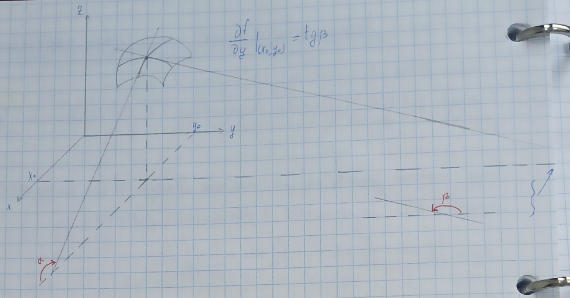
\includegraphics[max size={15cm}{10cm}]{7.8.1.png}
    \end{center}
    Пусть $z = f(x;y)$ дифференцируема в точке $(x_0; y_0)$.
    \[ \Delta z = \frac{\partial f}{\partial x} \Big|_{(x_0; y_0)} \Delta x + \frac{\partial f}{\partial y} \Big|_{(x_0; y_0)} \Delta y + o(\rho), \rho \to 0 \]
    \[ \Delta z = z - z_0 \]
    \[ \Delta y = y - y_0 \]
    \[ \Delta x = x - x_0 \]
    \[ z = z_0 + \frac{\partial f}{\partial x} \Big|_{(x_0; y_0)} (x-x_0) + \frac{\partial f}{\partial y} \Big|_{(x_0; y_0)} (y-y_0) + o(\rho) \,\,\,\,\, (1) \]
    Плоскость, определяемая уравнением
    \[ z = z_0 + \frac{\partial f}{\partial x} \Big|_{(x_0; y_0)} (x-x_0) + \frac{\partial f}{\partial y} \Big|_{(x_0; y_0)} (y-y_0) \,\,\,\,\, (2) \]
    называется \textbf{касательной плоскостью} к графику функции $z = f(x;y)$ в точке $(x_0; y_0)$.\\
    Обозначим в $(2)$ $z = z_{\text{кас}}$\\
    Тогда из $(1)$ и $(2)$ следует, что $z - z_{\text{кас}} = o(\rho), \rho \to 0$.
    \begin{center}
        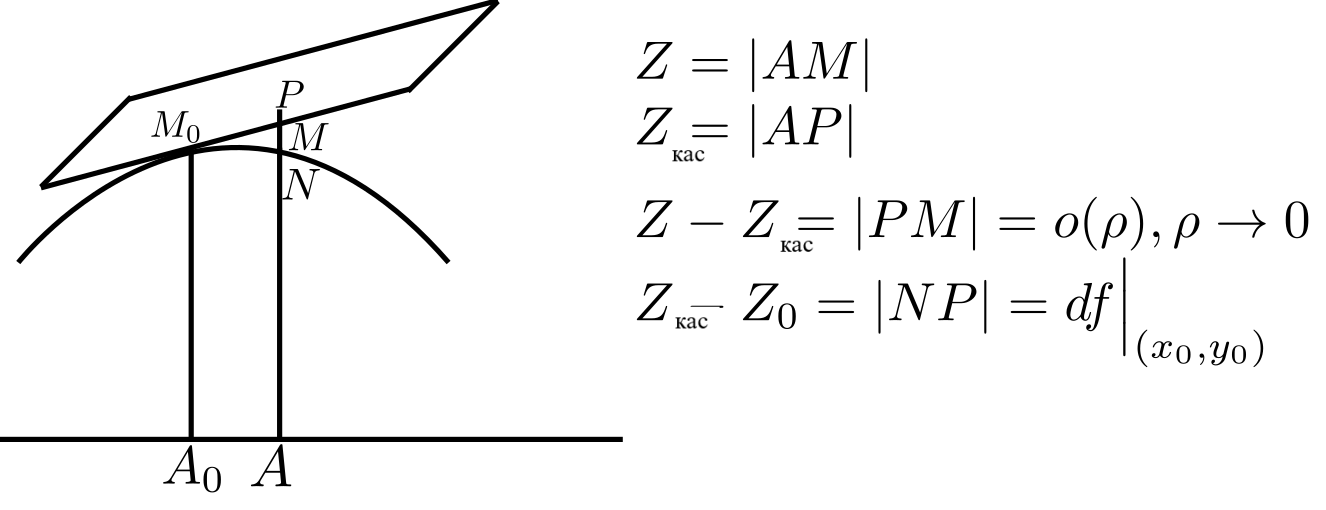
\includegraphics[max size={15cm}{10cm}]{7.8.2.png}
    \end{center}
    Рассмотрим $(2)$:
    \[ 1 \times z_{\text{кас}} = z + \underbrace{\frac{\partial f}{\partial x} \Big|_{(x_0; y_0)} (x-x_0) + \frac{\partial f}{\partial y} \Big|_{(x_0; y_0)} (y-y_0)} \]
    \[ z_{\text{кас}} = z_0 + df \Big|_{(x_0; y_0)} \]
    \[ df \Big|_{x_0; y_0} = z_{\text{кас}} - z_0 \]
    \[ \bar{n} \left(\frac{\partial f}{\partial x} \Big|_{(x_0; y_0)} (x-x_0); \frac{\partial f}{\partial y} \Big|_{(x_0; y_0)} (y-y_0); -1\right) \]
    Прямая вида
    \[ \frac{x - x_0}{\left( \frac{\partial f}{\partial x} \right) \Big|_{(x_0; y_0)}} = \frac{y - y_0}{\left( \frac{\partial f}{\partial y} \right) \Big|_{(x_0; y_0)}} = \frac{z - z_0}{-1} \]
    называется \textbf{нормалью} к поверхности $z = f(x; y)$ в точке $(x_0; y_0)$.\par\noindent
    \underline{Замечание:} если поверхность задана неявно $F(x,y,z) = 0$:
    \begin{adjustwidth}{1.5em}{1.5em}
        Уравнение касательной плоскости: 
        \[ \frac{\partial F}{\partial x} \Big|_{(x_0; y_0; z_0)} (x-x_0) + \frac{\partial F}{\partial y} \Big|_{(x_0; y_0; z_0)} (y-y_0) + \frac{\partial F}{\partial z} \Big|_{(x_0; y_0; z_0)} (z-z_0) = 0 \]
        Уравнение нормали:
        \[ \frac{x - x_0}{\left( \frac{\partial F}{\partial x} \right) \Big|_{M_0}} = \frac{y - y_0}{\left( \frac{\partial F}{\partial y} \right) \Big|_{M_0}} = \frac{z - z_0}{\left( \frac{\partial F}{\partial z} \right) \Big|_{M_0}} \]
    \end{adjustwidth}
    \subsubsection*{Частные дифференциалы}
    Если частное приращение функции $z = f(x;y)$ и $\Delta_x f$ можно представить в виде $\Delta_x f = A \Delta x + \varepsilon$, то $A \Delta x$ называются \textbf{частным дифференциалом} функции $f(x;y)$ в точке 
    \[ d_x f = A\Delta x = Adx = \frac{\partial f}{\partial x} \Big|_{M_0}dx \]
    Аналогично
    \[ d_y f = \frac{\partial f}{\partial y} \Big|_{M_0}dy \]
    Рассмотрим $z = f(x;y)$
    \[ dz = \frac{\partial f}{\partial x} \Big|_{M_0}dx + \frac{\partial f}{\partial y} \Big|_{M_0}dy = d_x f \Big|_{M_0} + d_y f \Big|_{M_0} \]
    $dz$ - полный дифференциал.

    \subsection{Применение дифференциалов в приближённых вычислениях.}\noindent
    Рассмотрим $f = f(x; y; z)$.\\
    Пусть $f$ дифференцируема в точке $M_0 (x_0; y_0; z_0)$.\\
    Тогда 
    \[ \Delta f = \frac{\partial f}{\partial x} \Big|_{M_0}dx + \frac{\partial f}{\partial y} \Big|_{M_0}dy + \frac{\partial f}{\partial z} \Big|_{M_0}dz + o(\rho), \rho \to 0\]
    \[ \Delta f = df \Big|_{M_0} + \cancel{o(\rho)}, \rho \to 0 \]
    \[ \underbrace{\Delta f}_{f - f_0} \approx df \Big|_{M_0} \]
    \[ \boxed{ f(x; y; z) \approx f(x_0; y_0; z_0) + \frac{\partial f}{\partial x} \Big|_{M_0}dx + \frac{\partial f}{\partial y} \Big|_{M_0}dy + \frac{\partial f}{\partial z} \Big|_{M_0}dz  } \]
    \underline{Пример:} вычислить приближённо.
    \begin{adjustwidth}{1.5em}{1.5em}
        \[ \frac{1.03^2}{\sqrt[3]{0.98} \times \sqrt[4]{1.05}} = ? \]
        Рассмотрим 
        \[ f(x; y; z) = \frac{x^2}{\sqrt[3]{y} \times \sqrt[4]{z}} \]
        \begin{gather*}
            x = 1.03 = x_0 + \Delta x = 1 + 0.03\\
            y = 0.98 = y_0 + \Delta y = 1 - 0.02\\
            z = 1.05 = z_0 + \Delta z = 1 + 0.05
        \end{gather*}
        \[ (x_0; y_0; z_0) = (1; 1; 1) \]
        \[ \Delta x = 0.03\,\, \Delta y = -0.02\,\, \Delta z = 0.05 \]
        \[ f(x_0; y_0; z_0) = 1 \]
        \begin{align*}
            \frac{\partial f}{\partial x} &= \frac{2x}{\sqrt[3]{y} \times \sqrt[4]{z}} & \frac{\partial f}{\partial x} \Big|_{M_0} &= 2\\
            \frac{\partial f}{\partial y} &= \frac{x^2}{\sqrt[4]{z}}\frac{(-\frac{1}{3})}{\sqrt[3]{y^4}} & \frac{\partial f}{\partial y} \Big|_{M_0} &= -\frac{1}{3}\\
            \frac{\partial f}{\partial z} &= \frac{x^2}{\sqrt[3]{y}}\frac{(-\frac{1}{4})}{\sqrt[4]{z^5}} & \frac{\partial f}{\partial z} \Big|_{M_0} &= -\frac{1}{4}\\
        \end{align*}
        \[ \frac{1.03^2}{\sqrt[3]{0.98} \times \sqrt[4]{1.05}} \approx 1 + 2 \times 0.03 - \frac{1}{3} \times (-0.02) - \frac{1}{4} \times 0.05 \approx 1.0482 \]
    \end{adjustwidth}

    \subsection{Производная по направлению функции в точке. Градиент функции в точке.}\noindent
    Рассмотрим функцию $f = f(x; y; z)$.\\
    Пусть она определена в окрестности точки $(x_0; y_0; z_0)$ и пусть задан произвольный вектор $\overline{l} \ne 0$.\\
    Пусть $\overline{l_0} = \frac{\overline{l}}{|\overline{l}|} = \underset{\text{направленные косинусы}}{\left( \overline{\cos \alpha; \cos \beta; \cos \gamma} \right)}$
    \begin{center}
        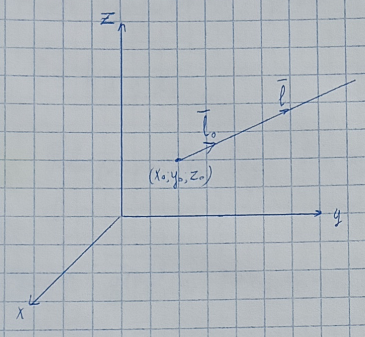
\includegraphics[max size={15cm}{10cm}]{7.10.1.png}
    \end{center}
    Запишем уравнение луча, выходящего из точки $(x_0; y_0; z_0)$ в направлении вектора $l$:
    \[ \frac{x - x_0}{\cos \alpha} = \frac{y - y_0}{\cos \beta} = \frac{z - z_0}{\cos \gamma} = t \]
    \[ \begin{cases}
        x = x_0 + t\cos \alpha\\
        y = y_0 + t\cos \beta\\
        z = z_0 + t\cos \gamma
    \end{cases}\,\,\,\,\, t \ge 0 \]
    \underline{Замечание:}
    \[ \sqrt{\cos^2 \alpha + \cos^2 \beta + \cos^2 \gamma} = 1\text{, т.к. } |\overline{l_0}| = 1 \]
    \[ \cos^2 \alpha + \cos^2 \beta + \cos^2 \gamma = 1\]
    \[ \sqrt{\frac{(x - x_0)^2}{t^2} = \frac{(y - y_0)^2}{t^2} = \frac{(z - z_0)^2}{t^2}} = 1 \]
    \[ \sqrt{(x - x_0)^2 = (y - y_0)^2 = (z - z_0)^2} = t\text{ - расстояние от точки } (x_0; y_0; z_0) \text{ до } (x; y; z) \]
    Рассмотрим $f(x;y;z)$ на построенном луче.\\
    Получится функция $f(x_0 + t\cos \alpha; y_0 + t \cos \beta; z_0 + t \cos \gamma)$.\par\noindent
    Производная сложной функции $f$ по переменной $t$ в точке $t = 0$ называется \textbf{производной функции} $f$ \textbf{в точке} $(x_0; y_0; z_0)$ \textbf{по направлению} $l$.
    \[ \frac{\partial f}{\partial l} \Big|_{(x_0; y_0; z_0)} = \frac{df}{dt}\Big|_{t_0} \]
    \begin{center}
        или
        \end{center}
    \[ \frac{\partial f}{\partial l} \Big|_{(x_0; y_0; z_0)} = \lim_{t \to 0}\frac{f(M) - f(M_0)}{t} \]
    Вычислим
    \begin{gather*}
        \frac{d}{dt}f(\underbrace{x_0 + \cos \alpha t}_x; \underbrace{y_0 + \cos \beta t}_y; \underbrace{z_0 + \cos \gamma t}_z) = \frac{\partial f}{\partial x} \frac{dx}{dt} + \frac{\partial f}{\partial y} \frac{dy}{dt} + \frac{\partial f}{\partial z} \frac{dz}{dt} =\\
        = \frac{\partial f}{\partial x} \cos \alpha + \frac{\partial f}{\partial y} \cos \beta + \frac{\partial f}{\partial z} \cos \gamma = \left( \overline{\frac{\partial f}{\partial x}; \frac{\partial f}{\partial y}; \frac{\partial f}{\partial z}} \right)\left( \overline{\cos \alpha; \cos \beta; \cos \gamma} \right) \boxed{=}
    \end{gather*}
    Вектор с координатами 
    \[ \left( \overline{\frac{\partial f}{\partial x}; \frac{\partial f}{\partial y}; \frac{\partial f}{\partial z}} \right) \]
    вычисленный в точке $(x_0; y_0; z_0)$, называется \textbf{градиентом} функции $f(x; y; z)$ в точке $(x_0; y_0; z_0)$.\\
    \underline{Обозначение:} $\overline{\text{grad}}f \Big|_{M_0}$.\par\noindent
    $\overline{\nabla}$ - \textbf{оператор Набла}.
    \[ \overline{\nabla} = \left( \overline{ \frac{\partial \sqcup}{\partial x}; \frac{\partial \sqcup}{\partial y}; \frac{\partial \sqcup}{\partial z} } \right) \]
    *вместо $\sqcup$ подставляем функцию (например, $f$), относительно которой применяем оператор Набла.
    \[ \overline{\nabla} f = \overline{\text{grad}}f\text{,} \]
    \[ \boxed{=} \, \boxed{ \overline{\text{grad}}f\Big|_{M_0} \times \overline{l_0} = \frac{\partial f}{\partial l}\Big|_{M_0} } \]
    \[ \overline{a}\overline{b} = |\overline{a}||\overline{b}|\cos(\underbrace{\overline{a}, \overline{b}}_{\varphi}) = \text{пр}_{\overline{b}} \overline{a} \times |\overline{b}| \]
    \begin{center}
        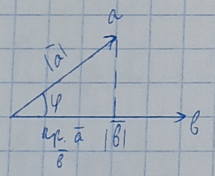
\includegraphics[max size={15cm}{10cm}]{7.10.2.png}
    \end{center}
    \[ \boxed{ \frac{\partial f}{\partial l} \Big|_{M_0} = \text{пр}_{\overline{l_0}}\overline{\text{grad}}f\Big|_{M_0} } \]
    \[ \frac{\partial f}{\partial l}\Big|_{M_0} = \overline{\text{grad}}f\Big|_{M_0} \times \overline{l_0} = |\overline{\text{grad}}f|\Big|_{M_0} \times |\underset{=1}{\overline{l_0}}| \times \cos \varphi \Rightarrow \frac{\partial f}{\partial l} \to \max \Longleftrightarrow \varphi = 0 \]
    Наибольшее значение $\frac{\partial f}{\partial l}\Big|_{M_0}$ будет иметь в направлении градиента в этой точке.\par\noindent
    \underline{Замечание:} Если $\overline{\nabla} f\Big|_{M_0} = \overline{0}$, то это значит, что производные функции по всем направлениям в этой точке равны $0$.

    \subsection{Линии и поверхности уровня}\noindent
    Рассмотрим $z = f(x;y)$.\\
    Линия вида $f(x;y) = \mathbb{C}$ называется \textbf{линией уровня от функции} $Z$.
    \begin{center}
        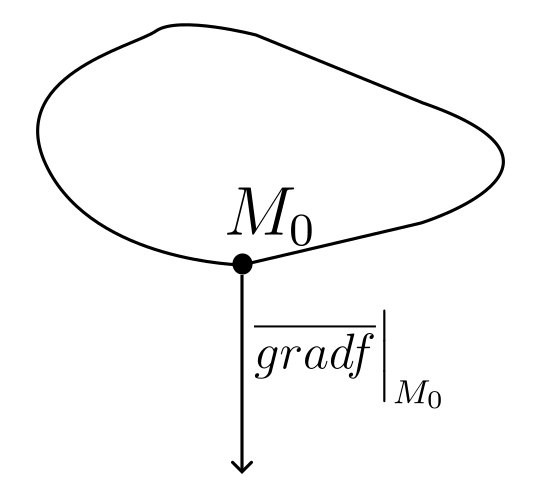
\includegraphics[max size={15cm}{10cm}]{7.11.1.png}
    \end{center}
    \[ \frac{x-x_0}{\frac{\partial f}{\partial x}} = \frac{y-y_0}{\frac{\partial f}{\partial y}} \]
    Вектор градиента функции в точке $M_0$ направлен перпендикулярно линии уровня.\\
    Рассмотрим $f = f(x;y;z)$.\\
    Поверхность вида $f(x;y;z) = \mathbb{C}$ называется \textbf{поверхностью уровня функции} $f$.\\
    Вектор $\overline{\text{grad}}f \Big|_{M_0}$ направлен по нормали к этой поверхности.

    \subsection{Частные производные и дифференциалы высших порядков}\noindent
    Рассмотрим $f = f(x;y)$. Имеем $\frac{\partial f}{\partial x}$; $\frac{\partial f}{\partial y}$.\\
    $\frac{\partial f}{\partial x}$ является функцией от $x$ и $y$: 
    \[ \frac{\partial f}{\partial x} = \frac{\partial f}{\partial x} (x; y) \]
    \[ \frac{\partial f}{\partial y} = \frac{\partial f}{\partial y} (x; y) \]
    Поэтому они тоже имеют частные производные.
    \begin{align*}
        f_{xx}'' &= (f'_x)'_x = \frac{\partial }{\partial x} \left( \frac{\partial f}{\partial x} \right) = \frac{\partial^2 f}{\partial x^2}; & f_{yy}'' &= (f'_y)'_y = \frac{\partial }{\partial y} \left( \frac{\partial f}{\partial y} \right) = \frac{\partial^2 f}{\partial y^2}\\
        f_{xy}'' &= (f'_x)'_y = \frac{\partial }{\partial y} \left( \frac{\partial f}{\partial x} \right) = \frac{\partial^2 f}{\partial y \partial x}; & f_{yx}'' &= (f'_y)'_x = \frac{\partial }{\partial x} \left( \frac{\partial f}{\partial y} \right) = \frac{\partial^2 f}{\partial x \partial y}
    \end{align*} 
    Аналогично определяются производные более высокого порядка.
    \[ \frac{\partial^5 f}{\partial x^5}; \frac{\partial^5 f}{\partial x^2 \partial y^3}; \frac{\partial^5 f}{\partial x \partial y \partial x \partial y \partial x}; \frac{\partial^2 f}{\partial x \partial y} \overset{?}{=} \frac{\partial^2 f}{\partial y \partial x} \]
    \subsubsection*{Теорема 7.12.1 (Шварца)}\label{th:7.12.1}
    Если функция определена вместе со своими частными производныи $f'_x; f'_y; f_{xy}''; f_{yx}''$ в некоторой окрестности точки $(x_0; y_0)$ и \underline{$f_{xy}''; f_{yx}''$ непрерывны} в этой точке, то:
    \[ \frac{\partial^2 f}{\partial x \partial y} \Big|_{(x_0; y_0)} = \frac{\partial^2 f}{\partial y \partial x} \Big|_{(x_0; y_0)} \]
    \underline{Доказательство:}
    \begin{adjustwidth}{1.5em}{1.5em}
        Рассмотрим повторные приращения:
        \[ \Delta_{xy} f = \Delta x (\Delta y f) = \Delta x [ f(x_0; y_0 + \Delta y) - f(x_0; y_0) ] = [ f(x_0 + \Delta x; y_0 + \Delta y) - f(x_0 + \Delta x; y_0) ] - [ f(x_0; y_0 + \Delta y) - f(x_0; y_0) ] \]
        \[ \Delta_{yx} f = \Delta y (\Delta x f) = \Delta y [ f(x_0 + \Delta x; y_0) - f(x_0; y_0) ] = [ f(x_0 + \Delta x; y_0 + \Delta y) - f(x_0; y_0 + \Delta y) ] - [ f(x_0 + \Delta x; y_0) - f(x_0; y_0) ] \]
        \[ \Delta_{xy}f = \Delta_{yx}f \]
        Обозначим
        \[ \varphi(x) = f(x, y_0 + \Delta y) - f(x; y_0) \]
        \[ \varphi'(x) = f'(x; y_0 + \Delta y) - f'(x;y_0) \]
        Тогда
        \begin{gather*}
            \Delta_{xy}f = \varphi (x_0 + \Delta x) - \varphi(x_0) \underset{Th. Лагранжа (4.12.4)}{=} \varphi'(\xi)\Delta x = \varphi'(x_0 + \theta_1 \Delta x)\Delta x =\\
            = [ f'_x(x_0 + \theta_1 \Delta x; y_0 + \Delta y) - f'_x(x_0 + \theta_1 \Delta x; y_0) ] \Delta x \underset{Th. Лагранжа (4.12.4)}{=}\\
            = f_{xy}''(x_0 + \theta_1 \Delta x; y_0 + \theta_2 \Delta y)\Delta x \Delta y
        \end{gather*}
        Аналогично 
        \[ \Delta_{yx}f = f_{yx}''(x_0 + \theta_3 \Delta x; y_0 + \theta_4 \Delta y)\Delta x \Delta y \]
        Т.к. $\Delta_{xy}f = \Delta_{yx}f$, то
        \[ f_{xy}''(x_0 + \theta_1 \Delta x; y_0 + \theta_2 \Delta y)\Delta x \Delta y = f_{yx}''(x_0 + \theta_3 \Delta x; y_0 + \theta_4 \Delta y)\Delta x \Delta y \]
        Т.к. $f_{xy}''; f_{yx}''$ непрерывны в точке $(x_0; y_0)$, то
        \[ \left.\begin{aligned}
            \lim_{\substack{\Delta x \to 0 \\ \Delta y \to 0}} f_{xy}'' (x_0 + \theta_1 \Delta x; y_0 + \theta_2 \Delta y) = f_{xy}'' (x_0; y_0)\\
            \lim_{\substack{\Delta x \to 0 \\ \Delta y \to 0}} f_{yx}'' (x_0 + \theta_3 \Delta x; y_0 + \theta_4 \Delta y) = f_{yx}'' (x_0; y_0)
        \end{aligned}\right\rbrace \Rightarrow f_{xy}'' (x_0; y_0) = f_{yx}''(x_0; y_0) \]
        \begin{center}
            \textbf{Ч.т.д.}
        \end{center}
    \end{adjustwidth}
    \textbf{Следствие:} в случае выполнения условий теоремы Шварца следует независимость результата дифференцирования от порядка переменных для функций любого числа переменных.
    \[ f_{xyz}''' = (f'_x)_{yz}'' = (f'_x)_{zy}'' = (f''_{xz})'_y = (f''_{zx})'_y = (f'_z)''_{xy} = (f'_z)''_{yx} \]
    \[ f_{xyz}''' = f_{zyx}''' \]
    \subsubsection*{Дифференциалы высших порядков}
    Рассмотрим $f = f(x_1; \dots; x_n)$.
    \[ df = \frac{\partial f}{\partial x_1}dx_1 + \frac{\partial f}{\partial x_2}dx_2 + \dots + \frac{\partial f}{\partial x_n}dx_n = \sum_{i=1}^{n}\frac{\partial f}{\partial x_i}dx_i \]
    \underline{Замечание:} в общем случае $df$ - функция $2n$ переменных $(x_1\, \dots\, x_n; dx_1\, \dots\, dx_n)$.\par\noindent
    Найдём второй дифференциал, рассматривая $df$ только как функцию $x_1\, \dots\, x_n$ (при фиксированных $dx_1\, \dots\, dx_n$).\\
    Обозначим дифференциал при повторном дифференцировании $\delta$:
    \[ \delta(df) = \sum_{i=1}^{n}\left[ \delta(\frac{\partial f}{\partial x_i}) \right] = \sum_{i=1}^{n} ( \sum_{j=1}^{n} \frac{\partial^2 f}{\partial x_j \partial x_i} \delta x_j )dx_i = \underbrace{\sum_{i=1}^{n} \sum_{j=1}^{n} \frac{\partial^2 f}{\partial x_j \partial x_i} dx_i \delta x_j}_{\substack{\text{билинейная форма} \\ \text{относительно переменных} \\ dx_1\, \dots\, dx_n;\,\, \delta x_1\, \dots\, \delta x_n}} \]
    Соответствующая билинейной форме квадратичная форма $(dx_1 = \delta x_1; dx_2 = \delta x_2; \dots; dx_n = \delta x_n)$ называется \textbf{вторым дифференциалом функции} $f$.
    \[ d^2 f = \delta (df) \Big|_{dx_i = \delta x_i} \]
    \[ d^2 f = \sum_{i=1}^{n} \sum_{j=1}^{n} \frac{\partial^2 f}{\partial x_i \partial x_j} dx_i dx_j \]
    Аналогично определяются дифференциалы более высокого порядка:
    \[ d^k f = \delta(d^{k-1}f)\Big|_{dx_i = \delta x_i} \]
    $y = f(x)$\\
    $dy = f'(x)dx$\\
    Рассмотрим $f = f(x_1\, \dots\, x_n)$:
    \[ d^k f = \left( \frac{\partial}{\partial x_1} dx_1 + \frac{\partial}{\partial x_2} dx_2 + \dots + \frac{\partial}{\partial x_n} dx_n \right)^{(k)}f \]
    $(k)$ - символическая степень.\par\noindent
    Рассмотрим $f = f(x;y)$:
    \begin{gather*}
            d^2 f=\left(\frac{\partial}{\partial x} d x+\frac{\partial}{\partial y} d y\right)^{(2)} f=\left(\frac{\partial^2}{\partial x^2} d x^2+2 \frac{\partial^2}{\partial x \partial y} d x d y+\frac{\partial^2}{\partial y^2} d y^2\right) f= \\
            = \frac{\partial^2 f}{\partial x^2} d x^2+2 \frac{\partial^2 f}{\partial x \partial y} d x d y+\frac{\partial^2 f}{\partial y^2} d y^2 \\
            d^3 f=\left(\frac{\partial}{\partial x} d x+\frac{\partial}{\partial y} d y\right)^{(3)} f=\frac{\partial^3 f}{\partial x^3} d x^3+3 \frac{\partial^3 f}{\partial x^2 \partial y} d x^2 d y+3 \frac{\partial^3 f}{\partial x \partial y^2} d x d y^2+\frac{\partial^3 f}{\partial y^3} d y^3
    \end{gather*}
    Рассмотрим $g = g(x; y; z)$:
    \begin{gather*}
        d^2 g=\left(\frac{\partial}{\partial x} d x+\frac{\partial}{\partial y} d y+\frac{\partial}{\partial z} d z\right)^2 g=\frac{\partial^2 g}{\partial x^2} d x^2+\frac{\partial^2 g}{\partial y^2} d y^2+\frac{\partial^2 g}{\partial z^2} d z^2+ \\
        +2 \frac{\partial^2 g}{\partial x \partial y} d x d y+2 \frac{\partial^2 g}{\partial x \partial z} d x d z+2 \frac{\partial^2 g}{\partial y \partial z} d y d z
    \end{gather*}
    Рассмотрим $f = f(x_1\, \dots\, x_n)$. Пусть $x_i = x_i(t_1\, \dots\, t_k)$ - зависимые переменные.
    \begin{gather*}
        d^2 f=\delta(d f) \Big|_{\delta x_i=d x_i}=\delta\left(\sum_{i=1}^n \frac{\partial f}{\partial x_i} d x_i\right)=\begin{vmatrix}d(u v)=u d v+v d u\\\\\end{vmatrix} \boxed{=} \\
        \boxed{=} \sum_{i=1}^n \frac{\partial f}{\partial x_i}\left(\delta d x_i\right)+\sum_{i=1}^n \delta\left(\frac{\partial f}{\partial x_i}\right) d x_i=\sum_{i=1}^n \frac{\partial f}{\partial x_i} d^2 x_i+\sum_{i=1}^n \sum_{i=j}^n \frac{\partial^2 f}{\partial x_j \partial x_i} d x_i d x_j
    \end{gather*}
    В случае зависимости переменных $x_i$ первая сумма $\ne 0$, т.е. второй дифференциал \underline{не обладает} свойством инвариантности формы записи относительно переменных.

    \subsection{Формула Тейлора для функции двух переменных}
    \subsubsection*{Теорема 7.13.1}\label{th:7.13.1}
    Пусть $f = f(x;y)$ непрерывна вместе со своими частными производными до $(n+1)$ порядка в окрестности точки $(x_0; y_0)$. Тогда $\forall\, \Delta x; \Delta y : \rho = \sqrt{\Delta x^2 + \Delta y^2} < \delta$ справедлива формула:
    \[ f(\underbrace{x_0 + \Delta x}_{x}; \underbrace{y_0 + \Delta y}_{y}) = \underbrace{ \sum_{k=0}^{n} \frac{d^k f \Big|_{(x_0; y_0)}}{k!} }_{\text{многочлен Тейлора}} + \underbrace{ \frac{d^{n+1} f \Big|_{(x_0 + \theta_1 \Delta x; y_0 + \theta_2 \Delta y)}}{(n+1)!} }_{\text{остаточный член в форме Лагранжа}} \]
    \begin{center}
        или
    \end{center}
    \[ f(x_0 + \Delta x; y_0 + \Delta y) = \sum_{k=0}^{n} \frac{1}{k!}\left( \frac{\partial }{\partial x}\Delta x + \frac{\partial }{\partial y}\Delta y \right)^{(k)} f \Big|_{(x_0; y_0)} + \underbrace{o(\rho^n)}_{\text{ост. член в форме Пеано}} \]
    \underline{Доказательство:}
    \begin{adjustwidth}{1.5em}{1.5em}
        Рассмотрим $F(t)$. Пусть $F(t)$ $(n + 1)$ раз дифференцируема в точке $t_0$. Тогда
        \[ F(t) = F(t_0) + \frac{F'(t_0)}{1!}(t-t_0) + \frac{F''(t_0)}{2!}(t-t_0)^2 + \dots + \frac{F^{(n)}(t_0)}{n!}(t-t_0)^n + \frac{F^{(n+1)}(\xi)}{(n+1)!}(t-t_0)^{n+1} \]
        \[ \underbrace{F(t) - F(t_0)}_{\Delta F} = \frac{1}{1!}dF\Big|_{t=t_0} + \frac{1}{2!}d^2F\Big|_{t=t_0} + \dots + \frac{1}{n!}d^nF\Big|_{t=t_0} + \frac{1}{(n+1)!}d^{n+1}F\Big|_{t=\xi} \]
        Рассмотрим $f = f(x; y)$. Пусть $M_0(x_0; y_0)$, $M(x; y) = M(x_0 + \Delta x; y_0 + \Delta y)$.\\
        Запишем уравнение отрезка $M_0M$ в параметрическом виде:
        \[ \frac{x - x_0}{x_1 - x_0} = \frac{y - y_0}{y_1 - y_0} \]
        \[ \frac{x - x_0}{\Delta x} = \frac{y - y_0}{\Delta y} = t \]
        Рассмотрим $f = f(x; y)$ вдоль отрезка $M_0M$:
        \[ f = f(x_0 + t \Delta x; y_0 + t \Delta y) \text{ - функция одной переменной} \]
        А для неё справедлива формула Тейлора ($t_0 = 0$).
        \[ \begin{cases}
            x = x_0 + t \Delta x\\
            y = y_0 + t \Delta y
        \end{cases}\,\,\, t \in [0; 1] \]
        \[ F(t) = F(0) + F'(0)t + \dots + \frac{1}{n!}F^{(n)}(0)t^n + \frac{1}{(n+1)!}F^{(n+1)}(\xi)t^{n+1} \]
        Рассмотрим
        \[ \Delta f = f(x_0 + \Delta x; y_0 + \Delta y) - f(x_0; y_0) = \overset{\xi \in (0; 1)}{F(1) - F(0)} \]
        \[ \Delta f = F(1) - F(0) = F'(0) + \frac{F''(0)}{2!} + \dots + \frac{F^{(n)}(0)}{n!} + \frac{F^{(n+1)}(\xi)}{(n+1)!} \]
        Найдём $F'(0)$:
        \[ F(t) = f(\underbrace{x_0 + t\Delta x}_{x}; \underbrace{y_0 + t\Delta y}_{y}) \]
        \begin{gather*}
            F'(t)=\frac{\partial f}{\partial x} \frac{d x}{d t}+\frac{\partial f}{\partial y} \frac{d y}{d t}=\frac{\partial f}{\partial x} \Delta x+\frac{\partial f}{\partial y} \Delta y=d f \quad F'(0)=d f \Big|_{(x_0, y_0)} \\
            F''(t)=\left(\frac{\partial f}{\partial x} \Delta x+\frac{\partial f}{\partial y} \Delta y\right)'_t =\left(\frac{\partial f}{\partial x}\right)'_t \Delta x+\left(\frac{\partial f}{\partial y}\right)'_t \Delta y= \\
            =\begin{vmatrix}
                \frac{\partial f}{\partial x}=\frac{\partial f}{\partial x}\left(x_0+t\Delta x, y_0+t \Delta y\right)\\
                \frac{\partial f}{\partial y}=\frac{\partial f}{\partial y}\left(x_0+t \Delta x, y_0+t \Delta y\right)
            \end{vmatrix} =\left[\frac{\partial^2 f}{\partial x^2} \Delta x+\frac{\partial^2 f}{\partial y \partial x} \Delta y\right] \Delta x+\left[\frac{\partial^2 f}{\partial x \partial y} \Delta x+\frac{\partial^2 f}{\partial y^2} \Delta y\right] \Delta y \boxed{=}  \\
            \boxed{=} \frac{\partial^2 f}{\partial x^2} \Delta x^2+2 \frac{\partial^2 f}{\partial x \partial y} \Delta x \Delta y+\frac{\partial^2 f}{\partial y^2} \Delta y^2=d^2 f \Rightarrow F^{\prime \prime}(0)=d^2 f \Big|_{(x_0, y_0)}
        \end{gather*}
        и т.д.
        \[ F^{(n)}(0) = d^n f \Big|_{(x_0; y_0)} \]
        \begin{center}
            \textbf{Ч.т.д.}
        \end{center}
    \end{adjustwidth}

    \subsection{Экстремум функции нескольких переменных}\noindent
    Рассмотрим $f = f(x_1\, \dots\, x_n)$. Пусть она определена в окрестности точки $(x^0_1\, \dots\, x^0_n)$.\\
    Точка $x^0$ называется \textbf{точкой локального максимума (минимума)}, если $\exists$ окрестность этой точки:
    \begin{align*} 
        \forall x = (x_1\, \dots\, x_n) \in \text{ окрестности } \quad &f(x) \le f(x^0) \\
        &(f(x) \ge f(x^0))
    \end{align*}
    \underline{Замечание:} если неравенство строгое, то точка $x^0$ называется точкой \textbf{строгого} локального максимума (минимума).\par\noindent
    Точки локального максимума и минимума функции называются \textbf{точками экстремума} функции.\\
    Точка $x^0$ называется точкой локального максимума (минимума), если $\exists$ окрестность этой точки такая, что $\Delta f = f(x) - f(x^0)$ не меняет знак.\\
    $\Delta f \ge 0$ - точка локального минимума.\\
    $\Delta f \le 0$ - точка локального максимума.
    \subsubsection*{Теорема 7.14.1 (необходимое условие экстремума)}\label{th:7.14.1}
    Если функция определена в окрестности точки экстремума $x^0$ и если в этой окрестности $\exists$ частная производная первого порядка $\frac{\partial f}{\partial x_i}\,(i = \overline{1;n})$, то все они равны нулю в этой точке.\par\noindent
    \underline{Доказательство:}
    \begin{adjustwidth}{1.5em}{1.5em}
        Пусть $i = 1$. Докажем, что $\frac{\partial f}{\partial x_1} \Big|_{x^0} = 0$.\\
        Зафиксируем координаты: $x_2 = x^0_2; x_3 = x^0_3; \dots; x_n = x^0_n$.\\
        Тогда $f = f(x_1, x^0_2, x^0_3, \dots, x^0_n)$ - функция одной переменной.\\
        Т.к. по условию точка $x^0 = (x^0_1, x^0_2, \dots, x^0_n)$ - точка локального экстремума функции $f(x_1\, \dots\, x_n)$, то точка $x^0_1$ - точка локального экстремума функции $f(x_1, x^0_2, \dots, x^0_n)$.\\
        Тогда по теореме Ферма (4.12.1):
        \[ \frac{df(x_1, x^0_2, \dots, x^0_n)}{dx_1} \Big|_{x_1 = x^0_1} = \frac{\partial f(x_1\, \dots\, x_n)}{\partial x_1} \Big|_{(x^0_1\, \dots\, x^0_n)} = 0 \]
        Аналогично можно доказать, что все остальные частные производные тоже равны нулю в точке $(x^0_1\, \dots\, x^0_n)$.
        \begin{center}
            \textbf{Ч.т.д.}
        \end{center}
    \end{adjustwidth}
    Точки, в которых все $\frac{\partial f}{\partial x_i} = 0 \quad i = \overline{1,n}$ называются \textbf{стационарными} точками функции $f$.\\
    Точки, в которых все частные производные равны нулю или не существуют, называются \textbf{критическими} точками функции $f$.\par\noindent
    \underline{Замечание:} пусть точка $x^0 = (x^0_1\, \dots\, x^0_n)$ - стационарная точка. Тогда
    \[ df \Big|_{x^0} = 0 \]
    \[ \overline{\text{grad}}f \Big|_{x^0} = \overline{0} \]
    \underline{Замечание:} условие равенства нулю всех частных производных в точке является необходимым условием, но не является достаточным.\\
    \underline{Пример:}
    \begin{adjustwidth}{1.5em}{1.5em}
        \begin{gather*}
            f = x^2 y\\
            \left.\begin{aligned}
                \frac{\partial f}{\partial x} = 2xy &= 0\\
                x^2 &= 0
            \end{aligned}\right\rbrace \Rightarrow \text{ точка } (0; 0) \text{ - стац. (одна из)}\\
            \frac{\partial f}{\partial y} = x^2 = 0
        \end{gather*}
        Рассмотрим $\Delta f$ в окрестности точки $(0; 0)$:
        \[ \Delta f = f(x) - f(x^0) = f(x_0 + \Delta x, y_0 + \Delta y) - f(\underset{= 0}{x_0};y_0) = (x_0 + \Delta x)^2 (y_0 + \Delta y) - x^2_0 y_0 = \boxed{\Delta x^2 \Delta y} \]
        Приращение $\Delta f$ в окрестности точки $(0; 0)$ имеет разные знаки $\Rightarrow$ точка $(0; 0)$ не является точкой экстремума.
    \end{adjustwidth}

    \subsection{Достаточные условия локального экстремума}\noindent
    Рассмотрим
    \begin{gather*}
        d^2 f \Big|_{x^0} = \sum_{i=1}^{n}\sum_{j=1}^{n} \frac{\partial^2 f}{\partial x_i \partial x_j} \Big|_{x^0} dx_i dx_j = \quad (x^0 \text{ - стац. точка})\\
        \sum_{i=1}^{n}\sum_{j=1}^{n}a_{ij}(x_i - x^0_i)(x_j - x^0_j) \text{ - квадратичная форма}
    \end{gather*}
    Рассмотрим $\Phi (h) = \Phi (h_1\, \dots\, h_n)$ - квадратичная форма.\\
    Если для любого набора $(h_1\, \dots\, h_n)$ $\Phi(h) > 0$, то квадратичная форма называется \textbf{положительно определённой}.\\
    Если для любого набора $(h_1\, \dots\, h_n)$ $\Phi(h) < 0$, то квадратичная форма называется \textbf{отрицательно определённой}.\\
    Рассмотрим $f = f(x_1\, \dots\, x_n)$:
    \[ d^2 f \Big|_{x^0} = \sum_{i=1}^{n}\sum_{j=1}^{n} \frac{\partial^2 f}{\partial x_i \partial x_j} \Big|_{x^0} dx_i dx_j = \sum_{i=1}^{n}\sum_{j=1}^{n}a_{ij}h_ih_j = \Phi(h_1\, \dots\, h_n) \]
    Если для любого набора $(h_1\, \dots\, h_n)$ $\Phi(h_1\, \dots\, h_n) > 0$, то квадратичная форма называется \textbf{положительно определённой}.\\
    Если для любого набора $(h_1\, \dots\, h_n)$ $\Phi(h_1\, \dots\, h_n) < 0$, то квадратичная форма называется \textbf{отрицательно определённой}.\\
    Если $\Phi(h_1\, \dots\, h_n)$ принимает как положительные значений, так и отрицательные, то квадратичная форма называется \textbf{знакопеременной}.\\
    Если для любого набора $(h_1\, \dots\, h_n)$ $\Phi(h_1\, \dots\, h_n) \underset{(\le 0)}{\ge 0}$, то квадратичная форма называется \textbf{квазизнакоопределённой}.\\
    Если $\Phi(h_1\, \dots\, h_n)$ принимает как положительные значений, так и отрицательные, так и нулевые значения, то квадратичная форма называется \textbf{квазизнакопеременной}.
    \subsubsection*{Теорема 7.15.1 (достаточные условия экстремума)}\label{th:7.15.1}
    Пусть $f = f(x_1\, \dots\, x_n)$ дважды непрерывно дифференцируема в окрестности критической точки $x^0 = (x^0_1; x^0_2; \dots; x^0_n)$. Тогда, если:
    \begin{enumerate}
        \item $d^2f \Big|_{x^0}$ является положительно определённой квадратичной формой, тогда $x^0$ - точка минимума.
        \item $d^2f \Big|_{x^0}$ является отрицательно определённой квадратичной формой, тогда $x^0$ - точка максимума.
        \item $d^2f \Big|_{x^0}$ является знакопеременной или квазизнакопеременной, тогда $x^0$ - не является точкой экстремума.
        \item $d^2f \Big|_{x^0}$ является квазизнакоопределённой, тогда необходимо провести дополнительное исследование на экстремум (по определению точки экстремума).
    \end{enumerate}
    Для определения знакоопределённости квадратичной формы используется \textbf{критерий Сильвестра}:
    \begin{adjustwidth}{1.5em}{1.5em}
        Обозначим: 
        \[ \frac{\partial^2 f}{\partial x_i \partial x_j} \Big|_{x^0} = a_{ij} \quad x^0 \text{ - стац. точка.} \]
        Составляем матрицу квадратичной формы второго дифференциала:
        \[
            \begin{pmatrix}
                a_{11} & a_{12} & \dots & a_{1n} \\
                a_{21} & a_{22} & \dots & a_{2n} \\
                \dots & \dots & \dots & \dots \\
                a_{n1} & a_{n2} & \dots & a_{nn} \\
            \end{pmatrix} 
        \]
        \begin{enumerate}
            \item Положительно определённая квадратичная форма (т. минимума): \[ \begin{pmatrix}
                + & & & \\
                & + & & \\
                & & \dots & \\
                & & & + \\
            \end{pmatrix} \]
            \item Отрицательно определённая квадратичная форма (т. максимума): \[ \begin{pmatrix}
                \overset{\text{обяз.}}{-} & & & & & \\
                & + & & & & \\
                & & - & & & \\
                & & & + & & \\
                & & & & - & \\
                & & & & & \dots \\
            \end{pmatrix} \]
            \item Знакопеременная квадратичная форма (экстремума нет): \[ \underset{\text{произвольное чередование + и -}}{\begin{pmatrix}
                + & & & & & & \\
                & + & & & & & \\
                & & - & & & & \\
                & & & - & & & \\
                & & & & + & & \\
                & & & & & - & \\
                & & & & & & \dots \\
            \end{pmatrix}} \]
            \item Квазиположительноопределённая квадратичная форма (требуется доп. исследование $\Rightarrow$ точка минимума или экстремума нет): \[ \begin{pmatrix}
                + & & & & & \\
                & + & & & & \\
                & & 0 & & & \\
                & & & + & & \\
                & & & & 0 & \\
                & & & & & \dots \\
            \end{pmatrix} \]
            \item Квазиотрицательноопределённая квадратичная форма (требуется доп. исследование $\Rightarrow$ точка максимума или экстремума нет): \[ \begin{pmatrix}
                - & & & & & & & & \\
                & + & & & & & & & \\
                & & 0 & & & & & & \\
                & & & 0 & & & & & \\
                & & & & - & & & & \\
                & & & & & + & & & \\
                & & & & & & 0 & & \\
                & & & & & & & + & \\
                & & & & & & & & \dots \\
            \end{pmatrix} \]
            \item Квазизнакопеременная квадратичная форма (экстремума нет): \[ \begin{pmatrix}
                + & & & & & & & & \\
                & - & & & & & & & \\
                & & - & & & & & & \\
                & & & 0 & & & & & \\
                & & & & - & & & & \\
                & & & & & - & & & \\
                & & & & & & 0 & & \\
                & & & & & & & + & \\
                & & & & & & & & \dots \\
            \end{pmatrix} \]
        \end{enumerate}
    \end{adjustwidth}
    
    \subsection{Неявные функции}\noindent
    Если $F(x;y)$ определена на некотором множестве $R_2$ и $\exists$ функция одной переменной, определённой на некотором $R_1$ и $F(x, f(x)) = 0$, то функция $f(x)$ называется \textbf{неявной функцией}, определённой уравнением $F(x;y) = 0$.
    \[ F(x;\underset{f(x)}{y}) = 0 = (x-x_0)^2 + (y-y_0)^2 \quad (x_0; y_0) \]
    \[ F(x;\underset{f(x)}{y}) = 0 = x^2 + y^2 + 1 \]
    \subsubsection*{Теорема 7.16.1 (о существовании неявной функции)}\label{th:7.16.1}
    Если $F(x;y)$ непрерывна в некоторой окрестности точки $(x_0; y_0)$ и $F(x_0; y_0) = 0$, $F'_y(x_0; y_0) \ne 0$, то $\exists$ $u(x_0)$ и $u(y_0)$ такие, что $\forall x \in u(x_0)$ $\exists$ единственное решение $y \in u(y_0)$ уравнения $F(x;y) = 0$\\
    Это решение обозначается $y = f(x)$. Оно непрерывно в $u(x_0)$ и $y_0 = f(x_0)$.\\
    Если дополнительно в окрестности точки $(x_0; y_0)$ $\exists$ непрерывная $F'_x(x; y)$, то функция $y = f(x)$ в точке $x_0$ имеет производную
    \[ \boxed{ y' = -\frac{F'_x}{F'_y} \Big|_{x_0; y_0} } \]
    \underline{Доказательство:}
    \begin{adjustwidth}{1.5em}{1.5em}
        Пусть $F(x; y)$ непрерывна в окрестности точки $(x_0; y_0)$.\\
        По условию $F'_y(x_0; y_0) \ne 0$. Пусть для определённости $F'_y(x_0; y_0) > 0$.\\
        По условию $F'_y$ непрерывна в точке $(x_0; y_0) \implies F'_y$ непрерывна в некоторой окрестности точки $(x_0; y_0)$ и (по теореме о сохранении знака (3.3.2)) $F'_y > 0$ в этой окрестности точки $(x_0; y_0)$.\\
        Т.к. $F'_y > 0 \implies F(x; y)$ возрастает по переменной $y$ на $[y_0 - \varepsilon; y_0 + \varepsilon]$ и $F(x_0; y_0) = 0$ по условию.\\
        Тогда $F(x_0; y_0 - \varepsilon) < 0$, $F(x_0; y_0 + \varepsilon) > 0$.\\
        Т.к. $F(x;y)$ непрерывна в окрестности точки $(x_0; y_0)$, то $\exists\, \delta$ такая, что в $u_\delta(x_0)$ функция $F(x; y)$ сохраняет такой же знак, как и в точке $(x_0; y_0 - \varepsilon)$ и $(x_0; y_0 + \varepsilon)$.\\
        Таким образом $\forall x \in (x_0 - \delta; x_0 + \delta)$ выполняется
        \begin{align*}
            F(x; y_0 - \varepsilon) < 0\\
            F(x; y_0 + \varepsilon) > 0
        \end{align*}
        Зафиксируем произвольное $x \in (x_0 - \delta; x_0 + \delta)$ и рассмотрим $F(x; y)$ функцию только переменной $y$ на $[ y_0 - \varepsilon; y_0 + \varepsilon ]$.\\
        Эта функция непрерывна, строго возрастает и имеет противоположные знаки на концах отрезка. Тогда по следствию из теоремы Больцано-Коши (3.8.3) $\exists$ значение $y^*$ (единственное) $\in (y_0 - \varepsilon; y_0 + \varepsilon)$ такое, что $F(x; y^*) = 0$.\\
        Таким образом определена однозначная функция такая, что каждому $x \in (x_0 - \delta; x_0 + \delta)$ соответствует единственное значение $y^* \in (y_0 - \varepsilon; y_0 + \varepsilon)$.\\
        Обозначим эту функцию $y^* = f(x)$.
        \[ \forall x \in (x_0 - \delta; x_0 + \delta) \quad F(x; y^*) = F(x; f(x)) = 0 \]
        Докажем, что $y^* = f(x)$ непрерывна в точке $x_0$: она непрерывна, т.к. 
        \[ \forall \varepsilon > 0\,\exists\,\delta > 0 : |x - x_0| < \delta \implies |y^* - f(x_0)| < \varepsilon \]
        Функция $y^* = f(x)$ будет непрерывна $\forall x \in (x_0 - \delta; x_0 + \delta)$.\\
        Пусть $x^* \in u(x_0; y_0)$. Всегда $\exists$ $u(x^*; y^*) < u(x_0; y_0)$. Тогда
        \[ \forall \varepsilon_1 > 0\, \exists\, \delta_1 > 0 : |x - x^*| < \delta_1 \implies | f(x) - f(x^*)| < \varepsilon_1 \]
        Т.е. $y^* = f(x)$ непрерывна в точке $x^* \implies$ она непрерывна $\forall x \in (x_0 - \delta; x_0 + \delta)$.\\
        Пусть функция $F(x; y)$ в $u(x_0; y_0)$ имеет непрерывную частную производную $F'_x$.\\
        Тогда по \hyperref[th:7.5.4]{достаточному условию дифференцируемости (7.5.4)} $F(x; y)$ дифференцируема в точке $(x_0; y_0)$.\\
        Тогда по определению дифференцируемости функции в точке
        \[ \Delta F = F'_x \Big|_{(x_0; y_0)} \Delta x + F'_y \Big|_{(x_0; y_0)} \Delta y + \overbrace{\varepsilon_1 \Delta x + \varepsilon_2 \Delta y}^{\text{\hyperref[th:7.5.1]{Th. 7.5.1}}} \]
        \[ F(\underset{=0}{x_0 + \Delta x}; y_0 + \Delta y) - F(\underset{=0}{x_0}; y_0) = F'_x \Big|_{(x_0; y_0)} \Delta x + F'_y \Big|_{(x_0; y_0)} \Delta y + \varepsilon_1 \Delta x + \varepsilon_2 \Delta y \]
        \underline{Замечание:} 
        \[ \begin{aligned}
            &f(x_0) = y_0\\
            &f(x_0 + \Delta x) = y_0 + \Delta y
        \end{aligned} \]
        Тогда
        \begin{gather*}
            F'_x \Big|_{(x_0; y_0)} \Delta x + F'_y \Big|_{(x_0; y_0)} \Delta y + \varepsilon_1 \Delta x + \varepsilon_2 \Delta y = 0 \quad \Big| : \Delta x\\
            F'_x \Big|_{(x_0; y_0)} + F'_y \Big|_{(x_0; y_0)} \frac{\Delta y}{\Delta x} + \varepsilon_1 + \varepsilon_2 \frac{\Delta y}{\Delta x} = 0\\
            \frac{\Delta y}{\Delta x} \left( F'_y \Big|_{(x_0; y_0)} + \varepsilon_2 \right) = - \left( F'_x \Big|_{(x_0; y_0)} + \varepsilon_1 \right)\\
            \frac{\Delta y}{\Delta x} = - \frac{F'_x \Big|_{(x_0; y_0)} + \varepsilon_1}{F'_y \Big|_{(x_0; y_0)} + \varepsilon_2}
        \end{gather*}
        \underline{Замечание:} $\rho = \sqrt{\Delta x^2 + \Delta y^2}$
        Т.к. функция $y^* = f(x)$ непрерывна в $u(x_0)$, то $\lim_{\Delta x \to 0} \Delta y = 0$.
        \[
            \lim_{\Delta x \to 0}\rho = \lim_{\Delta x \to 0} \sqrt{\Delta x^2 + \Delta y^2} = 0
        \]
        Рассмотрим
        \[ \lim_{\Delta x \to 0} \frac{\Delta y}{\Delta x} = \boxed{ - \frac{F'_x}{F'_y} \Big|_{(x_0; y_0)} = y' \Big|_{x^0} } \]
        \begin{center}
            \textbf{Ч.т.д.}
        \end{center}
    \end{adjustwidth}
    Рассмотрим $F(x; \underset{y(x)}{y}) = 0$
    \[ \frac{\partial f}{\partial x} + \frac{\partial f}{\partial y} \frac{dy}{dx} = 0 \]
    \[ y' = - \frac{F'_x}{F'_y} \]
    \subsubsection*{Теорема 7.16.2}\label{th:7.16.2}
    Пусть $F(x_1\, \dots\, x_n; y)$ определена в окрестности точки $(x^0_1\, x^0_2\, \dots\, x^0_n; y_0)$ и непрерывна вместе со своей частной производной $F'_y(x^0_1\, \dots\, x^0_n; y_0) \ne 0$ и $F(x^0_1\, x^0_2\, \dots\, x^0_n; y_0) = 0$. Тогда $\exists$ окрестность $u(x^0_1\, x^0_2\, \dots\, x^0_n)$ и $u(y_0)$ такие, что уравнение $F(x_1\, \dots\, x_n; y) = 0$ однозначно разрешимо в этих окрестностях.\\
    Это решение $y^* = f(x_1\, \dots\, x_n)$ непрерывно в $u(x^0_1\, \dots\, x^0_n)$.\\
    При дополнительном условии $F'_{x_i}$ непрерывна в точке $(x^0_1\, \dots\, x^0_n; y_0)$, функция $y^* = f(x_1\, \dots\, x_n)$ имеет в точке $(x^0_1\, \dots\, x^0_n)$ частную производную:
    \[ \frac{\partial f}{\partial x_i} = -\frac{F'_{x_i}}{F'_{y}} \quad i = \overline{1,n} \]
    Рассмотрим $F(x_1\, \dots\, x_n; y) = 0$.
    \[ \frac{\partial y}{\partial x_2} = \frac{\partial F}{\partial x_2} \times 1 + \frac{\partial F}{\partial y}\frac{\partial y}{\partial x_2} = 0 \]
    \[ \frac{\partial y}{\partial x_2} = -\frac{F'_{x_2}}{F'_y} \]
    \subsubsection*{Системы функций, заданных неявно}\noindent
    Рассмотрим совокупность неявных функций $y_1\, \dots\, y_n$, определяемых системой уравнений
    \[ \begin{cases}
        F_1(x_1\, \dots\, x_m; y_1\, \dots\, y_n) = 0\\
        F_2(x_1\, \dots\, x_m; y_1\, \dots\, y_n) = 0\\
        \dots\\
        F_n(x_1\, \dots\, x_m; y_1\, \dots\, y_n) = 0\\
    \end{cases} \]
    При определённых условиях эта система разрешима относительно функций
    \[ \begin{aligned}
        y_1 &= y_1(x_1\, \dots\, x_m)\\
        y_2 &= y_2(x_1\, \dots\, x_m)\\
        \dots\\
        y_n &= y_n(x_1\, \dots\, x_m)\\
    \end{aligned} \]
    Определитель вида
    \[ 
        \begin{vmatrix}
            \frac{\partial F_1}{\partial y_1} & \dots & \frac{\partial F_1}{\partial y_n}\\
            \frac{\partial F_2}{\partial y_1} & \dots & \frac{\partial F_2}{\partial y_n}\\
            \dots & \dots & \dots\\
            \frac{\partial F_n}{\partial y_1} & \dots & \frac{\partial F_n}{\partial y_n}\\
        \end{vmatrix}
    \]
    называется \textbf{определителем Якоби} или \textbf{Якобианом}
    \subsubsection*{Теорема 7.16.3}\label{th:7.16.3}
    Если функции $F_i(x_1\, \dots\, x_m; y_1\, \dots\, y_n) \quad i = \overline{1, n}$ имеют непрерывные частные производные в окрестности точки $M_0(x^0_1\, \dots\, x^0_m; y^0_1\, \dots\, y^0_n)$ и $F_i(M_0)=0$ и Якобиан $\frac{D(F_1\, \dots\, F_n)}{D(y_1\, \dots\, y_n)}\Big|_{M_0} \ne 0$, то $\exists$ окрестность $u(x^0_1\, \dots\, x^0_m)$ и $u(y^0_1\, \dots\, y^0_n)$ такие, что система уравнений $F_i(x_1\, \dots\, x_m; y_1\, \dots\, y_n) = 0 \quad i = \overline{1, n}$ однозначно разрешима в окрестности точки $M_0$ относительно переменных $y_1\, \dots\, y_n$, т.е. 
    \[ y^0_i = f_i(x_1\, \dots\, x_m) \quad i = \overline{1, n} \]
    Все $y^*_i$ имеют непрерывную частную производную в окрестностях $u(x^0_1\, \dots\, x^0_n)$.

    \subsection{Условный экстремум}\noindent
    Пусть задана функция $F = F(x_1\, \dots\, x_m; y_1\, \dots\, y_n)$\\
    \underline{Задача:} найти экстремум этой функции, если переменные $x_i, y_j$ связаны между собой уравнениями 
    \[ \begin{cases}
        f_1(x_1\, \dots\, x_m; y_1\, \dots\, y_n) = 0\\
        f_2(x_1\, \dots\, x_m; y_1\, \dots\, y_n) = 0\\
        \dots\\
        f_n(x_1\, \dots\, x_m; y_1\, \dots\, y_n) = 0\\
    \end{cases} \quad \text{\underline{условия связи}} \] 
    Точка $M_0 (x^0_1\, \dots\, x^0_m; y^0_1\, \dots\, y^0_n)$, \underline{удовлетворяющая условиям связи}, называется точкой \textbf{условного максимума (минимума)}, если $\exists$ окрестность точки $M_0$ такая, что 
    \[ \forall (x_1\, \dots\, x_m; y_1\, \dots\, y_n) \in u(M_0) : \underset{(F(M) \ge F(M_0))}{F(M) \le F(M_0)} \]
    \underline{Пример:}
    \begin{adjustwidth}{1.5em}{1.5em}
        Рассмотрим $F(x;y) = x^2 + y^2$. Найти экстремум $F$ при условии: $x + y - 1 = 0$.
        \begin{center}
            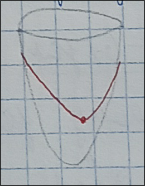
\includegraphics[max size={15cm}{10cm}]{7.17.1.png}
        \end{center}
        1 способ:
        \begin{gather*}
            y = 1 - x\\
            F(x, y(x)) = x^2 + (1 - x)^2 = x^2 + 1 - 2x + x^2 = 2x^2 - 2x + 1\\
            F' = 4x - 2 = 0
            x = \frac{1}{2}, y = 1 - x = \frac{1}{2}
        \end{gather*}
        Получили точку $\left( \frac{1}{2}; \frac{1}{2} \right)$
        \begin{center}
            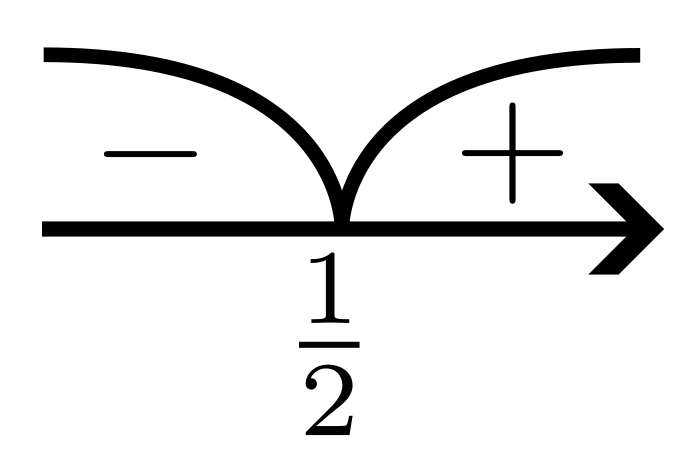
\includegraphics[max size={15cm}{10cm}]{7.17.2.png}
        \end{center}
        Ответ: точка $\left( \frac{1}{2}; \frac{1}{2} \right)$ - точка условного минимума.
    \end{adjustwidth}
    \underline{В общем виде:}
    \begin{adjustwidth}{1.5em}{1.5em}
        Рассмотрим $F(x_1\, \dots\, x_m; y_1\, \dots\, y_n) = F$\\
        Рассмотрим $f_i = f_i(x_1\, \dots\, x_m; y_1\, \dots\, y_n) = 0 \quad i = \overline{1, n}$ - условия связи.\\
        Пусть $\frac{D(f_1\, \dots\, f_n)}{D(y_1\, \dots\, y_n)} \Big|_{M_0} \ne 0$. Тогда по \hyperref[th:7.16.3]{теореме 7.16.3} система условий связи разрешима в окрестности точки $M_0$.
        \[ y_i = \varphi (x_1\, \dots\, x_m) \quad i = \overline{1, n} \]
        Все $y_i$ имеют непрерывную частную производную в точке $(x^0_1\, \dots\, x^0_n)$.\\
        Подставляя все $y_i$ в $F$, получим функцию переменных $x_1\, \dots\, x_n$.
        \[ F(x_1\, \dots\, x_m; y_1\, \dots\, y_n) = \Phi (x_1\, \dots\, x_m; y_1(x_1\, \dots\, x_m)\, \dots\, y_n(x_1\, \dots\, x_m)) = \Phi (x_1\, \dots\, x_m) \]
        Если $F$ достигает условного экстремума в точке $M_0 (x^0_1\, \dots\, x^0_m; y^0_1\, \dots\, y^0_n)$, то $\Phi$ достигает обычного экстремума в точке $P_0(x^0_1\, \dots\, x^0_m)$.\\
        Сложность - в разрешении системы условий связи.
    \end{adjustwidth}

    \subsection{Метод неопределённых множителей Лагранжа}\noindent
    Рассмотрим $F = F(x_1\, \dots\, x_m; y_1\, \dots\, y_n) \quad (1)$.
    \[ \begin{cases}
        f_1(x_1\, \dots\, x_m; y_1\, \dots\, y_n) = 0\\
        \dots\\
        f_n(x_1\, \dots\, x_m; y_1\, \dots\, y_n) = 0\\
    \end{cases} \quad (2) \]
    Пусть $M_0 (x^0_1\, \dots\, x^0_m; y^0_1\, \dots\, y^0_n)$ - точка условного экстремума.\\
    Тогда по необходимому условию экстремума:
    \[ 
        \begin{cases}
            \frac{\partial f_1}{\partial x_1}dx_1 + \frac{\partial f_1}{\partial x_2}dx_2 + \dots + \frac{\partial f_1}{\partial x_n}dx_m + \frac{\partial f_1}{\partial y_1}dy_1 + \dots + \frac{\partial f_1}{\partial y_n}dy_n = 0\\
            \dots\\
            \frac{\partial f_n}{\partial x_1}dx_1 + \frac{\partial f_n}{\partial x_2}dx_2 + \dots + \frac{\partial f_n}{\partial x_n}dx_m + \frac{\partial f_n}{\partial y_1}dy_1 + \dots + \frac{\partial f_n}{\partial y_n}dy_n = 0\\
        \end{cases} \quad (3)
    \]
    Получили систему $n$ уравнений $(n + m)$ неизвестных.\\
    По \hyperref[th:7.16.3]{теореме 7.16.3}:
    \[ \frac{D(f_1\, \dots\, f_n)}{D(y_1\, \dots\, y_n)} \ne 0 \implies \text{rang}(3) = n \]
    Тогда векторы $\overline{\text{grad}}f_1\, \dots\, \overline{\text{grad}}f_n$ являются линейно независимыми.\\
    Значит её можно выбрать в качестве базиса.\\
    Рассмотрим $(1)$. Т.к. $M_0$ - точка условного экстремума:
    \[ dF = 0 \implies \frac{\partial F}{\partial x_1}dx_1 + \frac{\partial F}{\partial x_2}dx_2 + \dots + \frac{\partial F}{\partial x_m}dx_m + \frac{\partial F}{\partial y_1}dy_1 + \dots + \frac{\partial F}{\partial y_n}dy_n = 0 \]
    Значит 
    \[ -\overline{\text{grad}}F = \lambda_1 \overline{\text{grad}}f_1 + \dots + \lambda_n \overline{\text{grad}}f_n \]
    \[ \overline{\text{grad}}(F + \lambda_1 f_1 + \lambda_2 f_2 + \dots + \lambda_n f_n) = 0 \]
    Функция $L = F + \lambda_1 f_1 + \lambda_2 f_2 + \dots + \lambda_n f_n$ называется \textbf{функцией Лагранжа}.\\
    $\lambda_1\, \dots\, \lambda_n$ - множители Лагранжа.\\
    Составим систему:
    \[ \begin{cases}
        \frac{\partial L}{\partial x_1} = \frac{\partial F}{\partial x_1} + \lambda_1 \frac{\partial f_1}{\partial x_1} + \dots + \lambda_n \frac{\partial f_n}{\partial x_1} = 0\\
        \dots\\
        \frac{\partial L}{\partial x_m} = \frac{\partial F}{\partial x_m} + \lambda_1 \frac{\partial f_1}{\partial x_m} + \dots + \lambda_n \frac{\partial f_n}{\partial x_m} = 0\\
        \frac{\partial L}{\partial y_1} = \frac{\partial F}{\partial y_1} + \lambda_1 \frac{\partial f_1}{\partial y_1} + \dots + \lambda_n \frac{\partial f_n}{\partial y_1} = 0\\
        \dots\\
        \frac{\partial L}{\partial y_n} = \frac{\partial F}{\partial y_n} + \lambda_1 \frac{\partial f_1}{\partial y_n} + \dots + \lambda_n \frac{\partial f_n}{\partial y_n} = 0\\
    \end{cases} \]
    Уравнений: $n + m$.\\
    \underline{Неизвестные:} $x_1\, \dots\, x_m, y_1\, \dots\, y_n, \lambda_1\, \dots\, \lambda_n \quad m + 2n$.\\
    Добавляем к этой системе уравнения связи
    \[ \begin{cases}
        f_1(x_1\, \dots\, x_m; y_1\, \dots\, y_n) = 0\\
        \dots\\
        f_n(x_1\, \dots\, x_m; y_1\, \dots\, y_n) = 0\\
    \end{cases} \]
    Получим $2n+m$ уравнений с $2n+m$ неизвестных.\\
    Для каждого набора $\lambda_1\, \dots\, \lambda_n$ будет найдена стационарная точка $(x^0_1\, \dots\, x^0_m; y^0_1\, \dots\, y^0_n)$.\\
    Применяя критерий Сильвестра при выполнении условий связи к функции Лагранжа, можно определить характер стационарной точки.\par\noindent
    \underline{Пример:}
    \begin{adjustwidth}{1.5em}{1.5em}
        Рассмотрим $F = x + y + z$.\\
        Условие связи: $xy + yz + xz = 3$.\\
        Найти условный экстремум.
        Решение: составим функцию Лагранжа.
        \[ L = x + y + z + \lambda (xy + yz + xz - 3) \]
        Составим систему
        \[ \left\lbrace\begin{aligned}
            \frac{\partial L}{\partial x} &= 1 + \lambda (y + z) = 0 & x &= y = z = -\frac{1}{2\lambda}\\
            \frac{\partial L}{\partial y} &= 1 + \lambda (x + z) = 0 & \lambda &= \pm\frac{1}{2}\\
            \frac{\partial L}{\partial z} &= 1 + \lambda (y + x) = 0 & \lambda_1 &=-\frac{1}{2}: \quad A(1; 1; 1)\\
            xy &+ yz + xz - 3 = 0 & \lambda_2 &= \frac{1}{2}: \quad B(-1; -1; -1)
        \end{aligned}\right. \]
        \begin{align}
            \frac{\partial^2 L}{\partial x^2} &= 0 & \frac{\partial^2 L}{\partial y^2} &= 0 & \frac{\partial^2 L}{\partial z^2} &= 0\\
            \frac{\partial^2 L}{\partial x \partial y} &= \lambda & \frac{\partial^2 L}{\partial x \partial z} &= \lambda & \frac{\partial^2 L}{\partial y \partial z} &= \lambda
        \end{align}
        \[ d^2 L = \left( \frac{\partial}{\partial x}dx + \frac{\partial}{\partial y}dy + \frac{\partial}{\partial z}dz \right)^{(2)}L = 2\lambda dx dy + 2\lambda dy dz + 2 \lambda dx dz \boxed{=} \]
        \[ xy + yz + xz - 3 = 0 \]
        \[ df = 0 \quad \frac{\partial f}{\partial x}dx + \frac{\partial f}{\partial y}dy + \frac{\partial f}{\partial z}dz = 0 \]
        \[ (y+z)dx + (x+z)dy + (x+y)dz = 0 \]
        В точках $A$ и $B$:
        \[ dx + dy + dz = 0 \]
        \[ dz = -(dx + dy) \]
        \[ \boxed{=} 2\lambda dxdy - 2\lambda dy(dx + dy) - 2\lambda dx(dx + dy) = -2 \lambda (dx^2 + dy^2 + dxdy) \]
        \[ \text{Точка }A \quad \begin{pmatrix}
            -2\lambda & -\lambda \\
            -\lambda & -2\lambda
        \end{pmatrix} = \begin{pmatrix}
            1 & \frac{1}{2}\\
            \frac{1}{2} & 1
        \end{pmatrix} = \boxed{ + } \implies \text{ точка } A \text{ - т. условного минимума.} \]
        \[ \text{Точка }B \quad \begin{pmatrix}
            -1 & -\frac{1}{2}\\
            -\frac{1}{2} & -1
        \end{pmatrix} = \boxed{ - } \implies \text{ точка } B \text{ - т. условного максимума.} \]
        \[ d^2 L > 0 \text{ для точки }A \]
        \[ d^2 L < 0 \text{ для точки }B \]
    \end{adjustwidth}
\end{document}